% ------------------------------------------------------------------------ %
% Modello di tesi di laurea o di dottorato
% di Luca Maggiori (C) 
%
% basato sul modello proposto da Lorenzo Pantieri
% (http://www.lorenzopantieri.net/LaTeX.html)
% e con la possibilità di attivare le impostazioni
% di impaginazione previste dal Politecnico di Milano
%
% versione 1.0	-- 4 maggio 2014
%	- prima versione completa
% versione 1.1	-- 5 maggio 2014
%	- aggiunta codici di esempio
%	- attivazione elenco dei codici
% ------------------------------------------------------------------------ %
%
%
% ------------------------------------------------------------------------ %
% Le impostazioni specifiche per il Politecnico di Milano
% sono definite sulla base del seguente documento:
% http://www.ingind.polimi.it/cms/file/1262/Norme_per_la_stesura_di_tesi_di_laurea_specialistica.pdf
% già presente nella cartella AltroMateriale
%
% Alcune delle impostazioni sono commentate e sostituite
% da altre ritenute in qualche modo 'migliori'; possono
% essere ripristinate commentando/decommentando i vari comandi
% ------------------------------------------------------------------------ %
%
%
% ------------------------------------------------------------------------ %
% I seguenti commenti speciali impostano:
% - applemac come codifica di input,
% - PDFLaTeX come motore di composizione;
% - Tesi.tex come documento principale;
% - il controllo ortografico italiano per l'editor.
%
% !TEX encoding = UTF-8 Unicode
% !TEX TS-program = pdflatex
% !TEX root = Tesi.tex
% !TEX spellcheck = it-IT
% ------------------------------------------------------------------------ %
%
%
% ------------------------------------------------------------------------ %
% 	PREAMBOLO
% ------------------------------------------------------------------------ %
%

%% IMPLEMENTATION %%
%--------------------------%
% Introduction 
% -> The BarbequeRTRM
% ---> Hardware reliability support
% -> DCWorms
% -> Hardware reliability monitoring (BSC?)
% Dynamic checkpoint-rate tuning
% -> Design
% -> Implementation
% The Reliam resource allocation policy
% -> Design
% -> Implementation in the BarbequeRTRM
% -> Implementation in DCWorms

%% EXPERIMENTAL RESULTS %%
%--------------------------%
% Single Node
% -> Checkpoint rate control
% -> Temperature/MTTF
% Multi Node
% -> Scalability
% Heterogeneous
% -> FPGA
% -> GPU



\documentclass[12pt,	% 10-11-12pt (12pt preferibile)
	a4paper,		%
	twoside,		% fronte-retro
	openright,		% nuovi capitoli iniziano nella pagina dispari
	titlepage,% 	% nuova pagina dopo il titolo (necessario per frontespizio)
	]{book}
%
% ------------------------------------------------------------------------ %
%
\usepackage[T1]{fontenc}		% codifica di output
%				% N.B. richiede una distribuzione completa di LaTeX
%
\usepackage[utf8]{inputenc}		% codifica di input; anche [latin1] va bene
%				% N.B. va accordata con le preferenze dell'editor
%
\usepackage[english]{babel}	% scelta lingua, sillabazione...
%				% l'ultima lingua (italiano) sarà la predefinita
%
\usepackage{microtype}		% micro-tipografia
\usepackage{lmodern}
\usepackage{nimbusmono}
\usepackage{enumitem}

% ------------------------------------------------------------------------ %
%
% 	LAYOUT - MARGINI - RILEGATURA
%
% -- AUTOMATICO
%\usepackage[binding=5mm]{layaureo} 	% margini ottimizzati per l'A4; rilegatura di 5 mm
%
% -- MANUALE (Impostazioni PoliMi)
\usepackage{geometry}
%
\geometry{verbose,	% verbose = displays the parameter results on the terminal
	top=43mm,	% margine superiore (PoliMi=43mm)
	bottom=44mm,	% margine inferiore (PoliMi=44mm)
	inner=41mm,	% margine interno pagina (PoliMi=41mm)
	outer=32mm,	% margine esterno pagina (PoliMi=32mm)
	bindingoffset=5mm,	% margine per la rilegatura
	heightrounded}
%
% ------------------------------------------------------------------------ %
%
%\usepackage[swapnames]{frontespizio}	% frontespizio (elegante ma non previsto al PoliMi)
%		% per includerlo nel documento bisogna:
%		% 1. compilare una prima volta Tesi.tex;
%		% 2. compilare a parte Tesi-frn.tex, generato dalla compilazione precedente;
%		% 3. compilare ancora Tesi.tex.
%		% Non è necessario fare questi passaggi altre volte
%		% se il frontespizio non è più modificato.
%
\usepackage{changepage,calc}                 % centra il frontespizio
%
\usepackage{emptypage}		% pagine vuote senza testatina e piede di pagina
%
\usepackage{indentfirst}		% rientra il primo paragrafo di ogni sezione
%
\usepackage{booktabs}		% tabelle (\toprule, \midrule, \bottomrule)
%
\usepackage{tabularx}		% tabelle di larghezza prefissata
%
\usepackage{graphicx}		% immagini
%
\usepackage[figuresright]{rotating}	% tabelle a 90 gradi
%
%\usepackage{subfig}			% sottofigure, sottotabelle
%
\usepackage{caption}		% didascalie
%
\usepackage{listings}		% codici
%
\usepackage[font=small]{quoting}	% citazioni
%
\usepackage{amsmath}	% matematica
%
\usepackage{amssymb}
\usepackage{mathtools}		% matematica
%
\usepackage{amsthm}		% matematica

\usepackage[output-decimal-marker={,}]{siunitx}	% SI (con separatore decimale=virgola)
%
\usepackage[italian]{varioref}		% riferimenti completi, con indicazione della pagina (\vref)
%
\usepackage{mparhack}	% finezze tipografiche (bug fixes di LaTeX)
%
\usepackage{relsize}			% make text larger or smaller than the surrounding text
% 				% \larger[i] \smaller[i]
%
% ------------------------------------------------------------------------ %
%
% 	BIBLIOGRAFIA
%
% adatta lo stile delle citazioni alla lingua corrente del documento
\usepackage[autostyle,italian=guillemets]{csquotes}
%
% pacchetto biblatex
%
% STILI di citazione:
%style=numeric-comp,	<-- ufficialmente richiesto dal PoliMi (numeri tra [ ])
% style=philosophy-modern,	<-- autore-anno (meno anonimo, più immediato e più elegante)
%
\usepackage[style=numeric-comp,	% numeric-comp oppure philosophy-modern,
	hyperref,			% riferimenti cliccabili
	backref,			% link alle pagine in cui il riferimento è citato
	natbib, 			% mantiene compatibilità con eventuali comandi natbib
	backend=biber,		% motore bibliografico (v. ArteLatex di Pantieri)
	defernumbers=true,	 	% riferimenti ordinati in ordine di comparsa
	]{biblatex}
%
\addbibresource{Bibliografia.bib}	% database bibliografico
%
% ------------------------------------------------------------------------ %
%
% Per generare effettivamente la bibliografia nel documento
% questa è la sequenza di composizione:
% 1. si compone il documento con LATEX una prima volta;
% 2. si lancia il programma Biber premendo l’apposito pulsante dell’editor;
% 3. si compone il documento altre 2 volte con LATEX (ma anche 3, NdA)
% Tale sequenza deve essere ripetuta solo se vengono fatte modifiche/aggiunte
% al database bibliografico.
%
% ------------------------------------------------------------------------ %
%
\usepackage[table,dvipsnames]{xcolor}	% colori - 68 colori predefiniti:
% 				% http://en.wikibooks.org/wiki/LaTeX/Colors
%
%\usepackage{subfig}

\newcommand{\multiref}[2]{\ref{#1} - \ref{#2}}

\usepackage{subcaption}

\usepackage{lipsum}			% testo fittizio
%
\usepackage{eurosym}		% simbolo dell'euro
%
\usepackage{hyperref}		% collegamenti ipertestuali
%
\usepackage{bookmark}		% gestione segnalibri del PDF
%
\usepackage{guit}			% simboli del Guit
%
\usepackage{fancyhdr}		% testatine e piede personalizzati
\setlength{\headheight}{15pt}
%
\usepackage{colortbl}		% per colorare i filetti delle tabelle
%
\usepackage[footnote,		% descrizione acronimo fatta a piè di pagina
	smaller,			% acronimo scritto con dimensione ridotta
	]{acronym}		% acronimi
%
\usepackage{multirow}		% celle tabelle alte più di una riga
%
\usepackage{pdfpages}		% inclusione di files pdf esterni
\usepackage{float}

\usepackage[linesnumbered,algoruled,noline]{algorithm2e}
\usepackage{algorithmic}
\usepackage{fancyvrb}
\usepackage{cprotect}

\newcommand\mycommfont[1]{\footnotesize\ttfamily{#1}}
\SetCommentSty{mycommfont}


\newcommand{\comment}[1]{}
\let\oldnl\nl% Store \nl in \oldnl
\newcommand{\nonl}{\renewcommand{\nl}{\let\nl\oldnl}}% Remove line number for one line

%
% ------------------------------------------------------------------------ %
% 	PREAMBOLO - SETUP
% ------------------------------------------------------------------------ %
%
% ------------------------------------------------------------------------ %
% !TEX encoding = UTF-8 Unicode
% !TEX TS-program = pdflatex
% !TEX root = Tesi.tex
% !TEX spellcheck = it-IT
% ------------------------------------------------------------------------ %
%
% ------------------------------------------------------------------------ %
% 	PREAMBOLO - SETUP
% ------------------------------------------------------------------------ %
% Comandi personali
% ------------------------------------------------------------------------ %
%
\newcommand{\myName}{Miriam Peta}			% autore
\newcommand{\myMatricola}{900122}			% matricola
\newcommand{\myTitle}{Modello di Tesi di Laurea in \LaTeX{}}	% titolo
\newcommand{\myUni}{Politecnico di Milano}		% università
\newcommand{\myFaculty}{Scuola di Ingegneria Industriale e dell'Informazione}	% facoltà/scuola
\newcommand{\myDegree}{Computer Science and Engineering}		% laurea
\newcommand{\myThesis}{Tesi di Laurea Magistrale}	% tipo di tesi
\newcommand{\myDepartment}{Dipartimento di Meccanica}	% dipartimento
\newcommand{\myProf}{Prof.~Charles~Dickens}		% relatore
\newcommand{\myOtherProf}{Ing.~Emilio~Salgari}		% eventuale correlatore
\newcommand{\myLocation}{Milano}			% dove
\newcommand{\myTime}{Aprile 2021}			% quando
\newcommand{\myAcademicYear}{2012--2013}		% anno accademico
\newcommand{\myLogo}{logoPoliMi}			% logo
\newcommand{\myLogoCFD}{logoPoliMiCFD}		% logo CFD :-)
\newcommand{\myUrlUni}{www.polimi.it}			% sito PoliMi
\newcommand{\myUrlFaculty}{www.ingindinf.polimi.it}	% sito Facoltà
%
% ------------------------------------------------------------------------ %
% Impostazioni di amsmath, amssymb, amsthm
% ------------------------------------------------------------------------ %
%
% un ambiente per i sistemi
\newenvironment{sistema}%
	{\left\lbrace\begin{array}{@{}l@{}}}%
	{\end{array}\right.}
%
% epsilon theta rho phi
\renewcommand{\epsilon}{\varepsilon}
\renewcommand{\theta}{\vartheta}
%\renewcommand{\rho}{\varrho}
\renewcommand{\phi}{\varphi}
%
\renewcommand{\vec}{\mathbf} 	% vettori in tondo nero
%
% ------------------------------------------------------------------------ %
% Impostazioni di biblatex
% ------------------------------------------------------------------------ %
%
% -- commentare o cancellare tutto se si desidera bibliografia standard
%
% I comandi seguenti saranno poi usati in Bibliografia.tex
% per suddividere i riferimenti bibliografici tra materiale citato
% e materiale non citato nel testo, con l'ulteriore distinzione in
% materiale cartaceo e materiale online (con link)
%
% Al termine si riportano anche pubblicazioni legate a Latex
% e alla stesura della tesi di laurea
%
\newcommand{\bibtitolocitati}{Riferimenti citati nel testo}
\newcommand{\bibtitolocitaticarta}{Pubblicazioni e Manuali}
\newcommand{\bibtitolocitatiweb}{Materiale Online}
\newcommand{\bibtitolononcitati}{Ulteriore materiale consultato}
\newcommand{\bibtitolononcitaticarta}{Pubblicazioni e Manuali}
\newcommand{\bibtitolononcitatiweb}{Materiale Online}
\newcommand{\bibtitololatex}{{\LaTeX{}}}
%
\DeclareBibliographyCategory{citati}
%
\defbibheading{citati-cartacei}{\subsection*{\bibtitolocitaticarta}}
\defbibheading{citati-web}{\subsection*{\bibtitolocitatiweb}}
\defbibheading{non-citati}{\section*{\bibtitolononcitati}}
\defbibheading{non-citati-cartacei}{\subsection*{\bibtitolononcitaticarta}}
\defbibheading{non-citati-web}{\subsection*{\bibtitolononcitatiweb}}
\defbibheading{latex}{\subsection*{\bibtitololatex}}
%
\AtEveryCitekey{\addtocategory{citati}{\thefield{entrykey}}}
%
\AtEveryBibitem{
    \clearfield{doi}
    \clearfield{eprint}
}
%
\nocite{*}	% manda in bibliografia anche tutte le opere non citate
%
% ------------------------------------------------------------------------ %
%
% Decommentare i comandi che seguono
% se si vuole ripristinare bibliografia standard
% (commentando tutto il blocco precedente)
%
%\defbibheading{bibliography}{%
%	\cleardoublepage%
%	\phantomsection%
%	\addcontentsline{toc}{chapter}{\bibname}%
%	\chapter*{\bibname\markboth{\bibname}{\bibname}}%
%	}
%
% ------------------------------------------------------------------------ %
% Impostazioni di xcolor
% ------------------------------------------------------------------------ %
%
% webcolors
\definecolor{webgreen}{rgb}{0,.5,0}
\definecolor{webbrown}{rgb}{.6,0,0}
%
% BluePolimi (colori delle presentazioni PPT del Politecnico di Milano)
\definecolor{darkbluePoliMi}{rgb}{0,0.18,0.40}	%rgb(0, 46, 103)
\definecolor{midbluePoliMi}{rgb}{0.33,0.47,0.62}	%rgb(84, 121, 157)
\definecolor{lightbluePoliMi}{rgb}{0.53,0.64,0.73}	%rgb(134, 163, 186)
\definecolor{orangePoliMi}{rgb}{1,0.59,0}		%rgb(255, 151, 0)
%
% redSapienza (rosso Sapienza)
\definecolor{redSapienza}{rgb}{0.514,0.031,0.165}	%rgb(131, 8, 42)
%
% ------------------------------------------------------------------------ %
% Impostazioni di listings
% ------------------------------------------------------------------------ %
%
\lstset{
	basicstyle=\smaller[0]\ttfamily,		% Black & White:
	keywordstyle=\color{RoyalBlue},	% keywordstyle=\color{black}\bfseries,
	commentstyle=\color{webgreen},	% commentstyle=\color{gray},
	stringstyle=\color{webbrown},		% stringstyle=\color{black},
	numbers=left,
	numberstyle=\smaller[2],
	stepnumber=1,
	numbersep=8pt,
	showspaces=false,
	showstringspaces=false,
	showtabs=false,
	breaklines=true,
	frameround=ffff,
	frame=single,
	tabsize=2,
	captionpos=t,
	breakatwhitespace=false,
	}
%
% Solution to the encoding issue
\lstset{literate=
  {á}{{\'a}}1 {é}{{\'e}}1 {í}{{\'i}}1 {ó}{{\'o}}1 {ú}{{\'u}}1
  {Á}{{\'A}}1 {É}{{\'E}}1 {Í}{{\'I}}1 {Ó}{{\'O}}1 {Ú}{{\'U}}1
  {à}{{\`a}}1 {è}{{\`e}}1 {ì}{{\`i}}1 {ò}{{\`o}}1 {ù}{{\`u}}1
  {À}{{\`A}}1 {È}{{\'E}}1 {Ì}{{\`I}}1 {Ò}{{\`O}}1 {Ù}{{\`U}}1
  {ä}{{\"a}}1 {ë}{{\"e}}1 {ï}{{\"i}}1 {ö}{{\"o}}1 {ü}{{\"u}}1
  {Ä}{{\"A}}1 {Ë}{{\"E}}1 {Ï}{{\"I}}1 {Ö}{{\"O}}1 {Ü}{{\"U}}1
  {â}{{\^a}}1 {ê}{{\^e}}1 {î}{{\^i}}1 {ô}{{\^o}}1 {û}{{\^u}}1
  {Â}{{\^A}}1 {Ê}{{\^E}}1 {Î}{{\^I}}1 {Ô}{{\^O}}1 {Û}{{\^U}}1
  {œ}{{\oe}}1 {Œ}{{\OE}}1 {æ}{{\ae}}1 {Æ}{{\AE}}1 {ß}{{\ss}}1
  {ç}{{\c c}}1 {Ç}{{\c C}}1 {ø}{{\o}}1 {å}{{\r a}}1 {Å}{{\r A}}1
  {€}{{\EUR}}1 {£}{{\pounds}}1
}
%
% Definizione ambienti per i vari linguaggi
%
\lstnewenvironment{Matlab}{\lstset{language=Matlab}}{}
%
\lstnewenvironment{C++}{\lstset{language=C++}}{}
%
\lstnewenvironment{bash}{\lstset{language=bash}}{}
%
%
% Comando per dare nome alla lista dei codici
%
\addto\captionsitalian{\renewcommand{\lstlistingname}{Codice}}
%
\addto\captionsitalian{\renewcommand{\lstlistlistingname}{Elenco dei codici}}
%
%\renewcommand{\lstlistingname}{Elenco dei codici}
%\renewcommand{\lstlistlistingname}{\lstlistingname}
%
% ------------------------------------------------------------------------ %
% Impostazioni di hyperref
% ------------------------------------------------------------------------ %
%
% per la descrizione delle varie opzioni vedere
% la guida del pacchetto hyperref
%
\hypersetup{
	%hyperfootnotes=false,
	%plainpages=false,
	%pdfpagelabels,
	colorlinks=true,
	linktocpage=true,	% true=link nei numeri pagina / false=link nel titolo
	pdfstartpage=1,
	pdfstartview=FitV,
	breaklinks=true,
	pageanchor=true,
	pdfpagemode=UseOutlines,
	%bookmarksnumbered,
	%bookmarksopen=true,
	bookmarksopenlevel=1,
	hypertexnames=true,
	pdfhighlight=/O,
	urlcolor=black,		% colore dei link a pagine web
	linkcolor=black,		% colore dei collegamenti nel testo
	citecolor=black,		% colore delle citazioni
	pdftitle={\myTitle},		% da qui in poi compilazione metadati
	pdfauthor={\textcopyright\ \myName, \myUni},
	pdfsubject={},
	pdfcreator={pdfLaTeX},
	pdfproducer={LaTeX with hyperref},
	pdfkeywords={polimi,
		tesi,
		latex,
		laurea,
		dottorato,
		scribd},
}
%
% comando per inviare mail
\newcommand{\mail}[1]{\href{mailto:#1}{\texttt{#1}}}
%
% Si possono avere tutti i collegamenti in nero e senza riquadri
% scrivendo semplicemente:
% \hypersetup{hidelinks}
%
% ------------------------------------------------------------------------ %
% Impostazioni di graphicx
% ------------------------------------------------------------------------ %
%
% Elenco dei percorsi in cui saranno cercate le immagini da inserire
%
% In questo modo non è necessario specificare il percorso relativo
% dell'immagine all'interno di \includegraphics{}, ma solo il nome.
%
% N.B. assicurarsi che non siano presenti più immagini
% con lo stesso nome.
%
\graphicspath{
	{Images/}
	{Images/Introduction/}
	{Images/StateOfTheArt/}
	{Images/Implementation/}
	{Images/ExperimentalEvaluation/}
	}
%
% ------------------------------------------------------------------------ %
% Impostazioni di caption
% ------------------------------------------------------------------------ %
%
\captionsetup{tableposition=top,
	figureposition=bottom,
	font=small,
	format=hang,
	labelfont=bf}
%
% ------------------------------------------------------------------------ %
% Impostazioni di fancyhdr
% ------------------------------------------------------------------------ %
%
% Impostazioni preferibili, ma NON del tutto adeguate alle norme POLIMI
% N.B. si possono usare queste impostazioni senza problemi anche per il PoliMi.
%
\pagestyle{fancy}			% sostituisce \pagestyle{header} standard
%
%\renewcommand{\chaptermark}[1]{	% ridefinisce indicazione capitolo
%	\markboth{\chaptername\ \thechapter.\ #1}{}}
%
\makeatletter 			% necessary for using \@chapapp
\renewcommand{\chaptermark}[1]{	% ridefinisce indicazione capitolo
  \markboth{\@chapapp\ \thechapter.\ #1}{}} % distinzione 'Capitolo' / 'Appendice'
\makeatother
%
\renewcommand{\sectionmark}[1]{	% ridefinisce indicazione sezione
	\markright{\thesection.\ #1}}
%
\fancyhf{}				% svuota testatine e piede
%
\fancyhead[LE,RO]{\scshape\thepage}	% numero pagine in alto
%
\fancyhead[LO]{\rightmark}	% info sezione nelle pag. dispari
%
\fancyhead[RE]{\scshape\leftmark}	% info capitolo nelle pag.pari
%
\renewcommand{\headrulewidth}{0.4pt}	% spessore linea header
%
\renewcommand{\footrulewidth}{0pt}	% spessore linea footer (0pt=nascosta)
%
\fancypagestyle{plain}{				% ridefinizione stile inizio capitolo
		\fancyhead{}			% header vuoto
		\fancyfoot[C]{\bfseries\thepage}		% numeri in grassetto al centro
		\renewcommand{\headrulewidth}{0pt}	% no linea
		}
%
% ------------------------------------------------------------------------ %
%
% Impostazioni maggiormente in linea con le norme POLIMI
% (decommentare l'intero blocco e commentare il blocco precedente)
%
% N.B. si possono usare le impostazioni precedenti senza problemi anche
% per il PoliMi (e infatti io ho usato le precedenti). Il mio consiglio è di
% usare, tra le 2 versioni proposte, quella sopra.
%
%\pagestyle{fancy}			% sostituisce \pagestyle{header} standard
%%
%\makeatletter 			% necessary for using \@chapapp
%\renewcommand{\chaptermark}[1]{%
%  \markboth{\@chapapp\ \thechapter.\ #1}{}} % distinzione 'Capitolo' / 'Appendice'
%\makeatother
%%
%\fancyhf{}				% svuota testatine e piede
%%
%\fancyfoot[LE,RO]{\bfseries\thepage}	% numero pagine in basso
%%
%\fancyhead[RO]{\bfseries\leftmark}	% info capitolo pagine dispari
%%
%\fancyhead[LE]{\bfseries\leftmark}	% info capitolo pagine pari
%%
%\renewcommand{\headrulewidth}{0.4pt}	% spessore linea header
%%
%\renewcommand{\footrulewidth}{0pt}	% spessore linea footer (0pt=nascosta)
%%
%\fancypagestyle{plain}{				% ridefinizione stile inizio capitolo
%		\fancyhf{}				% header e footer azzerati
%		\fancyfoot[C]{\bfseries\thepage}		% numero di pagina al centro
%		\renewcommand{\headrulewidth}{0pt}	% no linea header
%		}
%
% ------------------------------------------------------------------------ %
% Impostazioni degli acronimi
% ------------------------------------------------------------------------ %
%
% descrizione acronimi GIUSTIFICATA
\makeatletter
\def\bflabel#1{{\textbf{\textsf{#1}}\hfill}}
\renewenvironment{AC@deflist}[1]%
{\ifAC@nolist%
\else%
\begin{list}{}%
{\settowidth{\labelwidth}{\textbf{\textsf{#1}}}%
\setlength{\leftmargin}{\labelwidth}%
\addtolength{\leftmargin}{\labelsep}%
\renewcommand{\makelabel}{\bflabel}}%
\fi}%
{\ifAC@nolist%
\else%
\end{list}%
\fi}%
\makeatother
%
% ------------------------------------------------------------------------ %
% Altro
% ------------------------------------------------------------------------ %
%
% Gradiente
\newcommand{\gradiente}[1]{$\nabla #1$}
%
% puntini di omissione [...]
\newcommand{\omissis}{[\dots\negthinspace]}
%
% Eccezioni all'algoritmo di sillabazione
\hyphenation{OpenFOAM}
\hyphenation{Matlab}
\hyphenation{bash}
%
% ------------------------------------------------------------------------ %
% Finezze tipografiche per il Politecnico di Milano
% ------------------------------------------------------------------------ %
%
% Le seguenti modifiche possono essere commentate
% o adeguate ad un'altra università (es. 'Yale Blue'
% per l'università di Yale, 'Rosso Sapienza' per La Sapienza..)
%
% Filetti tabelle colorati
\arrayrulecolor{darkbluePoliMi}
%
%
% Righe delle note a piè di pagina colorate
\renewcommand{\footnoterule}{%
  \kern -3pt
  {\color{darkbluePoliMi} \hrule width 0.4\textwidth}
  \kern 2.6pt
}
\linespread{1.2}
%
% ------------------------------------------------------------------------ %		% file con le impostazioni personali
%
%
% ------------------------------------------------------------------------ %
% 	BEGIN DOCUMENT
% ------------------------------------------------------------------------ %
%

\comment{
\usepackage{titlesec}
\titleformat{\chapter}[display]
  {\bfseries\huge}
  {\filleft\Large\chaptertitlename~\Huge\thechapter}
  {3ex}
  {\titlerule\vspace{1.5ex}\filright}
  [\vspace{1ex}\titlerule]}
  
  \makeatletter
\let\ps@plain\ps@empty

\newcommand{\algrule}[1][.2pt]{\vskip.5\baselineskip\hrule height #1\vskip.5\baselineskip}
\makeatother
  
  \usepackage{titlesec}
\titleformat{\chapter}[display]
  {\scshape\huge}
  {\filleft\chaptertitlename~\fontfamily{lmr}\fontshape{sl}\fontsize{100}{90}\selectfont\thechapter}
  {1ex}
  {\titlerule\vspace{1.5ex}\filright}
  [\vspace{1ex}\titlerule]
 
  \comment{
  \usepackage{fix-cm}
\usepackage{xcolor}
\usepackage{titlesec}
\newcommand{\hsp}{\hspace{0pt}}
\titleformat{\chapter}[display]
{\flushright
\fontseries{b}\fontsize{80}{100}\selectfont}{\fontseries{b}\fontsize{100}{130}\selectfont\thechapter\hsp}{0pt}{\\ \Huge\bfseries}[]
}

\definecolor{lightblue}{RGB}{135,206,235}
\definecolor{odd}{RGB}{240,251,254}
\definecolor{even}{RGB}{225,247,253}
%\definecolor{odd}{RGB}{227,227,228}
%\definecolor{even}{RGB}{204,204,205}

\begin{document}
 %\setlength{\parindent}{0pt}
%
% ------------------------------------------------------------------------ %
% 	FRONTMATTER
% ------------------------------------------------------------------------ %
%
\frontmatter
%
%
% --------- CANCELLARE o COMMENTARE ---------------- %
%\thispagestyle{empty}
\pdfbookmark[1]{Frontespizio}{Frontespizio}
%
% ------------------------------------------------------------------------ %
% Frontespizio con pacchetto 'frontespizio'
% ------------------------------------------------------------------------ %
%
\begin{titlepage}
\newgeometry{top=2cm, 
    bottom=3cm,
	inner=41mm,	
	outer=32mm,	
	bindingoffset=5mm,
	heightrounded}
	\begin{center}
\begin{figure}
    \centering
    
\includegraphics[width=0.45\textwidth]{logo_poli.png}
\end{figure}
    \textsc{Scuola di\\Ingegneria Industriale e dell'Informazione}

\noindent\rule[0.5ex]{\linewidth}{0.4pt}
%\rule{\textwidth}{0.4pt}
%\end{center}
%\begin{center}
\textsc{Computer Science and Engineering\\Master's Thesis} \\
\end{center}
\vspace*{\fill}
\begin{center}
%\vspace{1.5cm} 
   %\textsc{\LARGE RELIAM}\\ 
   %\vspace{0.3cm}
   \textsc{\LARGE Reliability-aware\\ Resource Management for HPC Workload} \\
\end{center}
\vspace*{\fill}
\begin{flushright}
Author:\\
\textbf{Dott.ssa Miriam Peta}\\
Student ID:\\
\textbf{900122} \\ 
\end{flushright}
\vspace*{\fill}
Supervisor:\\
\textbf{Prof. William Fornaciari} \\
\newline
Co-Supervisor:\\
\textbf{Ph.D. Giuseppe Massari}

\vspace*{\fill}

\begin{center}
\textsc{Academic Year 2019/2020}\\
\end{center}
\restoregeometry
\end{titlepage}		% frontespizio figo ma non ufficiale al PoliMi

\cleardoublepage
% ------------------------------------------------------------------------ %
%
% Frontespizio ufficiale del Politecnico di Milano

%
% ------------------------------------------------------------------------ %
% !TEX encoding = UTF-8 Unicode
% !TEX TS-program = pdflatex
% !TEX root = ../Tesi.tex
% !TEX spellcheck = it-IT
% ------------------------------------------------------------------------ %
%
% ------------------------------------------------------------------------ %
% 	DEDICA
% ------------------------------------------------------------------------ %
%
\cleardoublepage
%
\phantomsection
%
\thispagestyle{empty}
%
\pdfbookmark{Dedica}{Dedica}
%
\vspace*{\stretch{1}}
%
\begin{flushright}
\textit{A me,}\\
\textit{che finalmente ci ho creduto.}
\end{flushright}
%
\vspace{\stretch{2}}
%
% ------------------------------------------------------------------------ %
%
% ------------------------------------------------------------------------ %
% !TEX encoding = UTF-8 Unicode
% !TEX TS-program = pdflatex
% !TEX root = ../Tesi.tex
% !TEX spellcheck = it-IT
% ------------------------------------------------------------------------ %
%
% ------------------------------------------------------------------------ %
% 	INDICI
% ------------------------------------------------------------------------ %
%
\cleardoublepage
%
% ------------------------------------------------------------------------ %
%
% Indice Generale
%
\pdfbookmark{\contentsname}{tableofcontents}
%
\setcounter{tocdepth}{2}
%
\tableofcontents
%
\cleardoublepage
%
% ------------------------------------------------------------------------ %
%
% Indice delle Figure
%
\phantomsection
%
\pdfbookmark{\listfigurename}{lof}
%
\listoffigures
%
\cleardoublepage
%
% ------------------------------------------------------------------------ %
%
% Indice delle Tabelle
%
\phantomsection
%
\pdfbookmark{\listtablename}{lot}
%
\listoftables
%
\cleardoublepage
%
% ------------------------------------------------------------------------ %
%
% Indice dei Listati di Programma
%
\phantomsection
%
%\pdfbookmark{\lstlistlistingname}{lol}
%
\listofalgorithms
%
\cleardoublepage
%
% ------------------------------------------------------------------------ %
%
% ------------------------------------------------------------------------ %
% !TEX encoding = UTF-8 Unicode
% !TEX TS-program = pdflatex
% !TEX root = ../Tesi.tex
% !TEX spellcheck = it-IT
% ------------------------------------------------------------------------ %
%
% ------------------------------------------------------------------------ %
% 	RINGRAZIAMENTI
% ------------------------------------------------------------------------ %
%
\cleardoublepage
%
\phantomsection
%
\pdfbookmark{Acknowledgements}{Acknowledgements}
%
\chapter*{Acknowledgements}
%
Questa tesi rappresenta il punto di arrivo del lungo viaggio che mi ha portata dall'essere una ragazzina impaurita di 19 anni, arrivata a Milano senza un'idea definita di dove stesse andando, alla donna consapevole e (perché no?) fiera che sono oggi. Se qualcuno avesse chiesto a quella ragazzina dove questo viaggio l'avrebbe condotta, probabilmente lei non avrebbe saputo rispondere. Se qualcuno le avesse chiesto dove \emph{sperava} che questo viaggio la conducesse, probabilmente la risposta sarebbe stata \emph{qui, dove sono oggi}. 

Grazie alla mia esperienza al Politecnico di Milano, sono riuscita a scoprire e applicare una passione che non sapevo neanche di avere, quindi, nonostante non sia una persona, il primo che voglio ringraziare per questo traguardo è sicuramente il \emph{Poli}, che, con le sue difficoltà e le sue opportunità, mi ha insegnato a non demordere se la ricompensa attesa è la propria soddisfazione. A questo riguardo, ringrazio mio fratello Emanuele, senza il cui intervento non avrei neanche sostenuto i test d'ingresso, e i miei genitori, che mi hanno sempre sostenuta e motivata non solo per tutta la durata del corso di studi, ma anche di tutta la mia vita.

Ringrazio tutti i miei compagni di corso, che mi hanno accompagnata nel viaggio e hanno condiviso con me gioie e dolori, in particolare Silvia, \emph{Fork}, la quale vicina e lontana è sempre stata presente. Ringrazio Sara, che non si è fermata alle apparenze, mi ha aiutata ad aprirmi e non mi ha mai mollata da allora. Le mie amiche Giulia, Martina, Chiara ed Eleonora e la mia coinquilina Simona, sulle quali ho sempre potuto contare. Ringrazio il mio ragazzo, Giovanni: nonostante il poco tempo e la distanza, la tua presenza è stata enorme.

Infine, un ringraziamento va al mio relatore, William Fornaciari, che mi ha permesso di conoscere i ragazzi dell'\emph{HeapLab}, in particolare Giuseppe, che mi ha seguita nel corso di questa tesi come un amico prima che come un correlatore: grazie per avermi accompagnata verso il traguardo.
\medskip



\bigskip
 
\noindent\textit{\myLocation, \myTime}
\hfill M.~P.
%
% ------------------------------------------------------------------------ %
%
% ------------------------------------------------------------------------ %
% !TEX encoding = UTF-8 Unicode
% !TEX TS-program = pdflatex
% !TEX root = ../Tesi.tex
% !TEX spellcheck = it-IT
% ------------------------------------------------------------------------ %
%
% ------------------------------------------------------------------------ %
% 	SOMMARIO + ABSTRACT
% ------------------------------------------------------------------------ %
\cleardoublepage
\phantomsection
\selectlanguage{italian}
%
\addcontentsline{toc}{chapter}{Sommario}
%
\chapter*{Sommario}
%
\markboth{Sommario}{Sommario}	% headings
%

Gli attuali domini applicativi dell'\emph{Information Technology} sono caratterizzati dalla generazione di quantità di dati sempre più ingenti, tali per cui il ricorrere a sistemi di High Performance Computing (HPC) diventa un requisito imprescindibile per l'analisi e il processing degli stessi \cite{marqube_2020}. La transizione verso l'exascale-grade HPC \cite{10.1145/3372390}, il numero sempre più alto di nodi e la fine delle leggi di scala di Dennard pongono nuove sfide riguardanti l'affidabilità delle applicazioni, eventualmente, parallele e dei componenti hardware sui quali vengono eseguite \cite{4629245}.

In risposta a tale problema, proponiamo un lavoro composto da due pilastri, il \emph{Dynamic Checkpoint Rate Tuning} e la \emph{Reliam Resource Allocation Policy}, progettati, implementati e integrati nel framework BarbequeRTRM, per migliorare, rispettivamente, la tolleranza ai guasti e l'affidabilità delle unità computazionali, il tutto tenendo in considerazione il loro impatto sulle performance. Da una parte, il Dynamic Checkpoint Rate Tuning consiste in un checkpoint scheduler \emph{intelligente} e \emph{application-aware}, la cui logica garantisce il soddisfacimento dei requisiti dell'applicazione in termini di frequenza di checkpoint, confinando l'overhead di quest'ultimo al di sotto di una soglia massima definita dall'utente. Dall'altra parte, la Reliam Resource Allocation Policy si serve di informazioni estratte a run time, derivanti dal monitoraggio delle risorse computazionali, al fine di effettuare un'allocazione delle risorse orientata all'affidabilità. Inoltre, ogni applicazione viene dotata di un controllore in grado di assegnare la  quantità di risorse computazionali, sulla base dei requisiti di performance e dell'utilizzo specifico di ogni singola applicazione e/o dell'intero sistema. Il risultato ricercato dalla Reliam Resource Allocation Policy è il miglioramento non solo dell'affidabilità delle applicazioni, che verranno eseguite dagli elementi di elaborazione definiti \emph{non critici} attraverso un profiling periodico, ma anche in termini di rallentamento dell'usura dei componenti hardware. Infine, la presenza di un controllore personalizzabile, permette la minimizzazione dell'utilizzo della CPU, prevedendo contestualmente l'attribuzione di priorità a una o più applicazioni sulle altre.

\selectlanguage{english}
%\endgroup

%\vfill
%
% ------------------------------------------------------------------------ %
%
% ------------------------------------------------------------------------ %
% !TEX encoding = UTF-8 Unicode
% !TEX TS-program = pdflatex
% !TEX root = ../Tesi.tex
% !TEX spellcheck = it-IT
% ------------------------------------------------------------------------ %
%
% ------------------------------------------------------------------------ %
% 	SOMMARIO + ABSTRACT
% ------------------------------------------------------------------------ %

\phantomsection
%
\addcontentsline{toc}{chapter}{Abstract}
%
\chapter*{Abstract}
%
\markboth{Abstract}{Abstract}	% headings
%
In today’s world, larger and larger amounts of data are constantly being generated, processed and analyzed, placing High Performance Computing (HPC) systems at the core of major advances in a variety of application areas \cite{marqube_2020}. The transition to exascale-grade HPC \cite{10.1145/3372390}, the increasing number of nodes and the loss of Dennard scaling pose new challenges with respect to the reliability of possibly parallel applications and of the hardware components they run on \cite{4629245}. 

As a response to such problem, we propose a work composed of two pillars, the \emph{Dynamic Checkpoint Rate Tuning} and the \emph{Reliam Resource Allocation Policy}, designed, implemented and integrated in the BarbequeRTRM framework, to enforce, respectively, fault tolerance and reliability, both of them without neglecting their impact on the performance. On one hand, the Dynamic Checkpoint Rate Tuning consists in a \emph{smart} and \emph{application-aware} checkpoint scheduler, whose logic guarantees the application requirements in terms of checkpoint rate, while bounding its overhead under a user defined threshold. On the other hand, the Reliam Resource Allocation Policy makes use of run time information coming from the monitoring of the computing resources, in order to carry out a reliability-aware resource binding. Moreover, a controller is provided to the each application of the system, in order to quantify the \emph{CPU quota} to assign, meeting application-specific and/or system wise performance and usage objectives.  The result the Reliam Resource Allocation Policy wants to achieve is an improvement not only in the reliability of the applications, which are going to be executed on the processing elements marked as \emph{not critical} by means of a periodical profiling, but also in the slowdown of the hardware components aging. Finally, the presence of a customized controller, upon which use-cases are provided as a guideline on the controlling parameters, allows the minimization of the CPU utilization, while permitting the prioritization of one or more application with respect to the others.

%\endgroup

%\vfill
%
% ------------------------------------------------------------------------ %
%
\cleardoublepage
%
% ------------------------------------------------------------------------ %
% 	MAINMATTER
% ------------------------------------------------------------------------ %
%
\mainmatter
%
% ------------------------------------------------------------------------ %
% !TEX encoding = UTF-8 Unicode
% !TEX TS-program = pdflatex
% !TEX root = ../Tesi.tex
% !TEX spellcheck = it-IT
% ------------------------------------------------------------------------ %
%
% ------------------------------------------------------------------------ %
% 	introduction
% ------------------------------------------------------------------------ %
%

\cleardoublepage
%
\phantomsection
%
%\addcontentsline{toc}{chapter}{Introduction}
%
\chapter{Introduction}
%
%\markboth{Introduction}{Introduction}	% headings
%
\label{cap:introduction}

\section{High Performance Computing}
The term High Performance Computing (HPC) refers to the use of supercomputers in order to solve computational problems either too complex to be solved by standard machines or extremely expensive in terms of time. Supercomputers are clusters of nodes, provided with a number of processors able to communicate with each other and to share resources as efficiently as possible.

Nowadays, with the growing number of large-scale simulations and data-intensive critical applications, e.g. deep learning training models, HPC plays an increasingly important role in many application areas \cite{marqube_2020}.

More and more often, HPC systems complement the use of traditional CPUs with accelerators such as GPUs, which offer a huge processing power thanks to the large number of cores, and FPGA, which can be adapted to specific tasks, favoring the heterogeneity of the system itself.

However, the technology enhancement, the increasing number of nodes and the loss of Dennard scaling \cite{10.1145/2024723.2000108} are introducing many challenges in power distribution and dissipation \cite{article}, dependability and resilience \cite{inproceedings}, resource allocation scheduling \cite{4629245} and parallel programming models \cite{Shalf2010ExascaleCT}.

\subsection{HPC Systems Architectures}
Intel distinguishes three main classes of HPC design, depending on the application area \cite{intel}:
\begin{description}
\item [Parallel Computing.] It aggregates the computing power of dozens or hundreds of processors located in a single physical system executing calculations simultaneously. It allows the computation of big and complex problems, splitting the workload into separate tasks carried out simultaneously.
\item [Cluster Computing.] It combines the processing capability of many independent computers linked together through a local-area network (LAN), acting like a single one. This configuration aims to solve a single problem spanning it across the nodes of the system, defining a specific network topology and organization in order to maximize the processing speed.
\item [Grid/Distributed Computing.] It connects multiple computers through a network to solve a complex problem or performing a large computational task. This approach allows to address jobs that can be split into separate chunks and distributed across the grid. Each node performs tasks independently without the need of communicating with the other nodes. 
\end{description}

\begin{figure}[t]
    \centering
    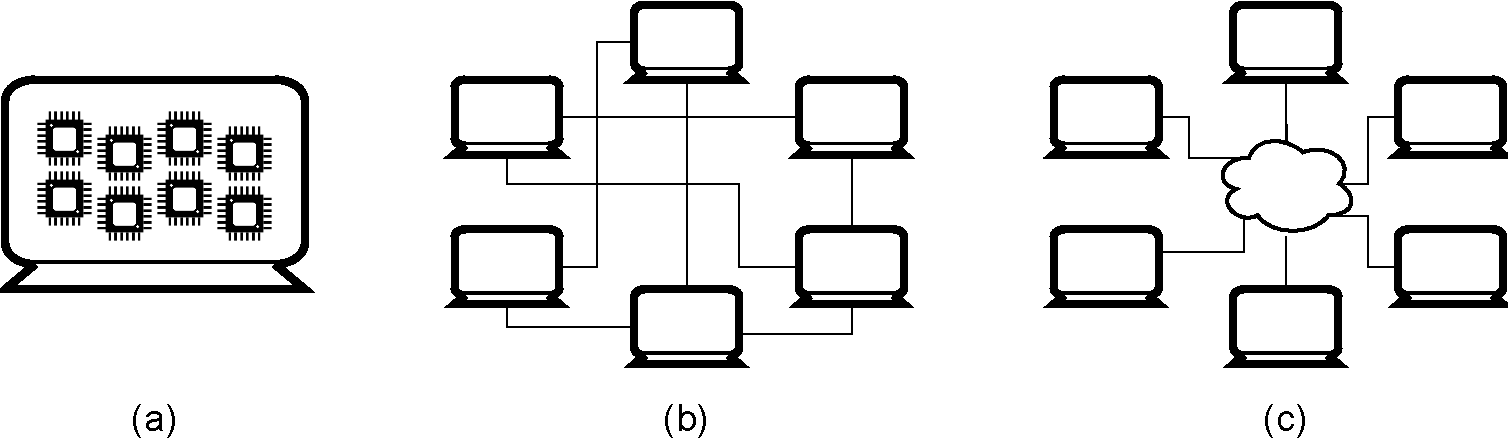
\includegraphics[width=\textwidth]{HPC_architectures.pdf}
    \caption{HPC system architectures: (a) Parallel Computing, (b) Cluster Computing, (c) Grid/Distributed Computing.}
    \label{fig:hpcarch}
\end{figure}

It becomes clear that architectural choices, including the hardware components to employ, play a fundamental role in the design of a HPC system.

At the time of writing, on one hand, Intel proposes the 3rd generation of Xeon Scalable processors. More specifically, Intel Xeon Platinum 8300 processors, the HPC flagship line of the company, offers up to 28 cores with the highest supported frequency of 4.3 GHz.

On the other hand, AMD, with its 2nd generation of EPYC High frequency processors, offers up to 64 cores with the highest supported frequency of 3.4GHz. Both solutions are provided with a DDR4 with the highest memory speed of 3200 MT/s.

With respect to the communication, in HPC systems, the nodes are usually connected via high speed networks, typically 10Gigabit Fiber Optics Ethernet or InfiniBand, which is used for data interconnect both among and within computers.

Storage is also a major matter of focus: Network Attached Storage (NAS) and Storage Area Network (SAN) are currently the most used solutions. NAS allows data to be stored in a centralized fashion in order to be accessible by all the nodes of the network and supports Redundant Array of Independent Disks (RAID) solutions to ensure data security. While NAS focuses on ease of use, manageability and scalability, SAN points its attention to high performance, low latency and lower total cost of ownership. It offers any-to-any connectivity among servers and storage devices, improving backups and redundancy. Either way, it is important that storage performance and capacity scale linearly with the numbers of nodes and disks.

\section{Reliability in HPC Systems}
With the arrival of exascale-grade High Performance Computing \cite{10.1145/3372390}, reliability becomes a matter of big concern at different scales: failures and downtimes have a severe impact on the performance of parallel programs, while the presence of a multitude of hardware and software components make failure and reliability prediction a challenging problem \cite{4629245}. 

Reliability concerns affect not only supercomputers but also data centers. More advanced technologies with higher susceptibility to radiation and aging, the use of larger memories, as well as the effect of other semiconductor components, such as processors and GPUs, can only lead to much higher hardware-related failure rates in the future \cite{10.1145/3403956}.
In the next paragraphs, the terminology of the paper \textit{Dependable Computing and Fault Tolerance: Concepts and Terminology} \cite{532603} will be followed to address  the various attributes of computing systems dependability.

\subsection{Faults, errors and failures}
A \emph{fault} is defined as the cause originating one or several latent \emph{errors} in the component where it occurs. An example of fault might be a programmer's mistake or a short occurring in an integrated circuit causing a connection stuck at a Boolean value. At some point, the latent error might be activated, becoming effective, and it might propagate from one component to another. Keeping on the examples above, the error in the written software or the stuck-at fault may become effective through the activation of the module in which the error resides, determining a mistaken output. A \emph{failure} occurs when the dysfunctions in the underlying architecture begin to deviate the behavior of higher-level modules, affecting the delivered service. Figure~\ref{fig:chain} summarize what Avizienis et al. \cite{1335465} define as the \emph{fundamental chain of dependability and security threats}: white arrows express causality relationship between fault, errors and failure. 

From the failure domain viewpoint, one can distinguish between:
\begin{figure}
    \centering
    
\includegraphics[width=\textwidth]{fault_error_failure.pdf}
    \caption{The fundamental chain of dependability and security threats.}
    \label{fig:chain}
\end{figure}
\begin{description}
    \item [Content failures.] Deviation of the content of the information from the golden (non-faulty) execution.
    \item [Timing failures.] Arrival time and/or duration of the execution different from the golden one. They can be distinguished in \emph{early} and \emph{late} depending on when the service is delivered.
\end{description}

Failures where both content and timing constraints are not satisfied fall in two classes:
\begin{description}
\item[Halt failures.] The service is halted, system activity is no longer observable by the user, external state becomes constant.
\item[Erratic failures.] The provided service is erratic and/or under-performing.
\end{description}
\begin{figure}[t]
    \centering
    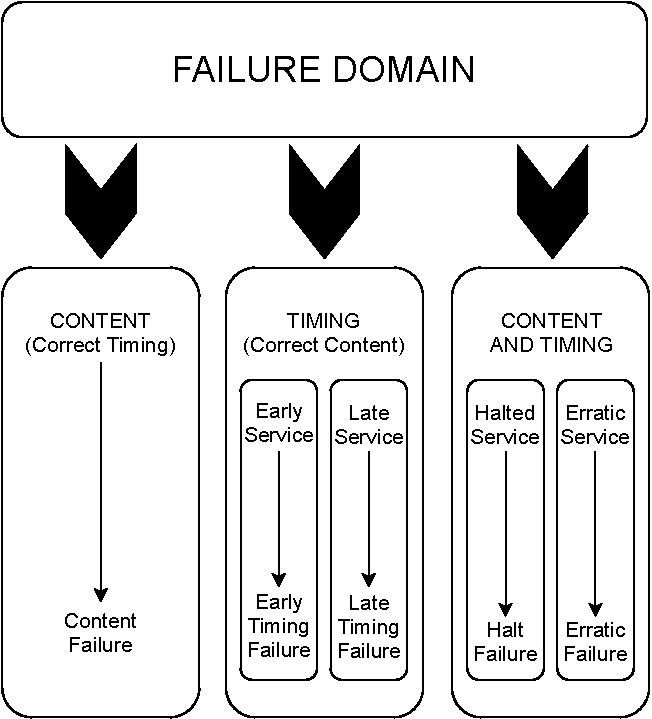
\includegraphics[width=0.7\textwidth]{failure_domain.pdf}
    \caption{Service failure modes with respect to the failure domain viewpoint.}
    \label{fig:failure_domain}
\end{figure}
Figure~\ref{fig:failure_domain} summarizes the service failure modes with respect to the failure domain viewpoint.

Both timing and/or content errors can be classified in the following categories:
\begin{description}
    \item [Silent Data Corruption (SDC).] The error is not detected but data is corrupted.
    \item [Detected Unrecoverable Error (DUE).] The error is detected, but it cannot be corrected.
    \item [Corrected Errors (CE).] The error is corrected and content and timing are recovered.
\end{description}

\subsection{Fault sources in HPC}
Reliability has been acknowledged as a major roadblock for HPC applications in current supercomputers and data centers. Although solution to ensure fault tolerance have been already developed, faults are still a huge source of issues in nowadays HPC systems.

As the HPC centers get larger, the probability of errors increases proportionally to the number of components \cite{10.1145/3403956}. Moreover, miniaturization causes smaller devices to be subject to increasing current densities at relatively high temperatures. In this scenario, thermal aging becomes a major concern: Bias Temperature Instability (BTI), is one of the most relevant aging effects in CMOS technology \cite{10.1145/3403956}. A sudden increase in temperature might result in charges being trapped in the transistor gate oxide reducing the voltage threshold of the transistors consequently affecting the maximum frequency of the circuit. BTI not only generates a faulty transient effect, present until the system is switched off, but also increases the probability and intensity of this effect as the system ages. In recent years, more and more HPC applications need strict timing requirements which would be endangered by this problem \cite{reghenzani2020timing}.

Canal et al. in \cite{10.1145/3403956} explains how thermal stress reduces the Mean Time To Failure (MTTF) of the system, but reducing hot spots is a not sufficient solution to cope with high performance CPUs thermal management: dynamic behaviors of temperature, summarized below, have a strong impact on the reliability of HPC processors and need to be taken into account.
\begin{description}
\item[Temporal Temperature Gradient (TTG).] Defined as the rate in which temperature changes over time, it depends on the workload capacity of each processing element and its operating frequency. It has a severe impact on the lifetime of the system.
\item[Spatial Temperature Gradient (STG).] It is the difference in temperature between two distinct points of the circuit. It also affect the system lifetime reliability, but, differently from TTG, it is mostly caused by power and thermal throttling at processor level.
\item[Thermal Cycling (TC).] As the name suggests, it consists in a periodic increasing and decreasing of the circuit temperature. It may be caused by power saving techniques as Dynamic Voltage and Frequency Scaling (DVFS) or the switching on and off of the processing elements. It poses a more serious impact on the MTTF as the amplitude of the cycles increases.
\end{description}

\subsection{The heterogeneity challenge}
HPC systems revealed themselves as a fundamental instrument in the resolution of problems in a variety of scientific fields, supporting research and innovation  by increasing exploration speed and effectiveness, nevertheless, the demand for a higher-performance supercomputer keeps increasing \cite{10.1145/3372790}. Particularly, the importance of heterogeneity is sensibly growing. The introduction and diffusion of GPUs as processing units is leaving a great mark in the performance of parallel computing, such that it is reasonable to think that they will be more and more used in the future. Originally, GPUs had been designed to improve image rendering, a field of application in which reliability was not a topic of main importance, since it was intrinsically fault tolerant \cite{Fang12evaluatingthe}. However, in the recent years, General Purpose GPUs (GPGPUs) are becoming a powerful resource in HPC systems, where the complexity of the hardware and the extensive number of components  considerably enlarges the probability of failures, making indispensable a concern in such regard.

Cini et al., in \cite{10.1145/3372790}, listed a series of reasons why heterogeneous systems, more specifically GPU based, are less reliable than homogeneous ones, CPU based:
\begin{description}
\item [Massive Parallelism.] An application running on a GPU can consists of millions of independent thread which means that the failure of one of them does not affect any of the others. The problem is that an error can propagates very quickly if not detected in time and, if it lies on shared resources, it may affect also other nodes. In this circumstances, a failure is very costly compared to an homogeneous system. Moreover, experimental studies show that memory errors are likely to disturb multiple threads or multiple thread blocks.
\item[High Density.] Since a GPU is made up of a large number of execution units (EUs) it may reach a very high temperature. If a 12-core CPU contains about 72 EUs, GPUs can consist of more than 3000 EUs, which, if working in parallel, might cause the system to overheat with a probability of causing failures 10x higher than CPUs.
\item[High Utilization.] The number of GPUs is growing in heterogeneous systems and the huge number of cores makes systems more susceptible to failures. Furthermore, applications running on GPUs are destined to become increasingly popular, intensifying the utilization and, consequently, the error rate. 
\end{description}

Beside GPU accelerators technology, architectural specialization is another exploited option in HPC to face the slow down in Moore’s Law: in recent years, the use of FPGA technology is catching on to improve performance and lower energy costs \cite{insidehpc_2019}. Edward Stott et al., in \cite{5694288}, identify Negative-Bias Temperature Instability (NBTI) the primary degradation mechanism of FPGA, finding that the generated wear out speed strongly depends on the supply voltage and temperature. 
Amouri et al. carried out an experimental analysis \cite{6927390}, from which resulted that after just one week of  continuous stress, FPGA had shown an aging extent of up to 5.17\%, correlating the problem to the effect of the Input Signal Probability (SP) and the effect of the Switching Activity (SA).

As shown, the progress in HPC systems comes with the need of a particular attention to the problem of the reliability towards the hardware components that constitute them and, consequently, towards the applications that run on them, which is the main concern at the base of the presented work. 

\section{Thesis objectives and structure}
This thesis work aims to cope at software level with the reliability issues of HPC systems, through the design, implementation and integration in the BarbequeRTRM of a scheduling policy able to proactively minimize the degradation of the hardware components, while ensuring a backup plan in case of occurrence of failures. This purpose will be achieved taking care as much as possible of the reliability-performance trade off and exploiting a resource allocation algorithm, able to adapt itself not only to the specific machine in which it runs, but also to the process to execute. 

The thesis is organized as it follows: 
\begin{description}
\item[{\hyperref[cap:stateofart]{State of the Art.}}] In this chapter an overview on the Checkpoint/Restart technique and the Run Time Resource Managers, pillars on which the project presented by this thesis is built, is given, highlighting the limits of the state of the art.
\item[{\hyperref[cap:implementation]{Design and Implementation.}}] In this chapter the design and the implementation of the Dynamic Checkpoint Rate Tuning and of the Reliam Resource Allocation Policy, the two main components of this work, are deeply examined, with a focus on the framework in which they have been integrated, i.e. the BarbequeRTRM.
\item[{\hyperref[cap:experimental]{Experimental Evaluation.}}] In this chapter the series of experiments performed on the Dynamic Checkpoint Rate Tuning and on the Reliam Resource Allocation Policy will be described, analyzed and commented. Through those tests, not only a measurement of the effectiveness of the proposed work will be extract, but also some guideline in the choice of the parameters at users discretion.
\end{description}
%\cleardoublepage
%
\phantomsection
\chapter{State of the Art}
%
\label{cap:stateofart}
This chapter presents the state of the art concerning the areas which this thesis contribution is focused on. 

In the first part of the chapter, an overview on the Checkpoint/Restart technique is provided, with a brief summary of some of the most known technologies used to implement it.

The second part of the chapter will, instead, focus on the Run-Time Resource Management and its correlation with the resource allocation problem.

\section{Checkpoint/Restart}
\label{sec:criu}
\begin{figure}
    \centering
    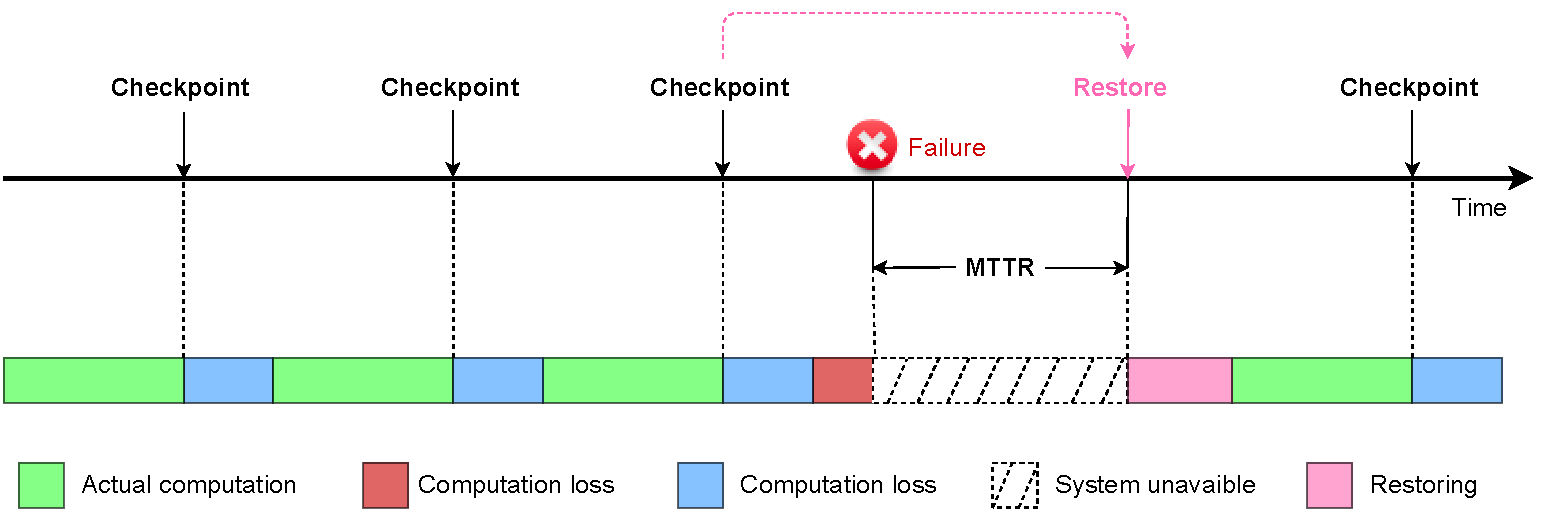
\includegraphics[width=\textwidth]{chk_rst.pdf}
    \caption{The Checkpoint/Restart approach.}
    \label{fig:chkrst}
\end{figure}
As anticipated in {\hyperref[cap:introduction]{Chapter 1}}, reliability is nowadays playing an increasingly fundamental role in HPC systems and, in this scenario, the importance of fault tolerance mechanisms is growing with the advancing of the computing potential of such systems. For this reason, many technique have been implemented to improve reliability and availability of parallel and  possibly distributed contexts: \emph{rollback-recovery} techniques are one of the most used solution for long running application.

\emph{Application Checkpointing} is the act of saving a snapshot of the state of a computation in order to be able, in case of failure, to resume it with the least possible computation loss. Walters et al., in \cite{app-checkpoint}, highlight that, from a high level perspective, three main steps are needed to perform a checkpoint:
\begin{enumerate}
    \item Interrupt the computation.
    \item Save the address space to a file.
    \item Save the register set to a file.
\end{enumerate}
\emph{Checkpoint/Restart (C/R)} is a widespread rollback-recovery technique which resorts to Application Checkpointing in order to enforce fault tolerance of computing systems. A summary of the approach provided by C/R is depicted in Figure~\ref{fig:chkrst}. C/R tools save the state (\emph{image}) of the processes in a non-volatile storage so that, when a system failure occurs, the image can be recovered and used to restart the execution from the saved checkpoint state.

When considering clusters of machines, each of which with a different failure rate, new problems arise. If a single application makes use of an entire cluster for its execution, synchronization among the machines is needed. Generally, C/R tools follow the three steps listed below \cite{reghenzani_2016}:
\begin{enumerate}
    \item Synchronization of the application processes execution to reach a global consistent state (\emph{sync}).
    \item Application execution state saving (\emph{checkpoint}).
    \item Application execution resuming (\emph{restart}).
\end{enumerate}
Depending on the level in which they operate, C/R tools are divided in four main categories and result transparent to the other layers \cite{app-checkpoint}:
\begin{description}
    \item[Hardware-level.] In this configuration, additional hardware is integrated with the processor to execute the checkpointing routine.
    \item[Kernel-level.] The operating system is in charge of the execution of the checkpointing code.
    \item[User-level.] An external library is linked to the program and is responsible for the checkpointing process.
    \item[Application-level.] The checkpointing code is inserted in the application code by the programmer.
\end{description}
At the time of writing, C/R routines are very expensive in terms of time stolen from the actual computation: the overall overhead  may reach over the 50\% of the total execution time \cite{6468485}.

In the years, several software tools implementing the Checkpoint/Restart mechanism have been distributed: an overview of some of the most known ones is provided below.

\begin{description}
    \item[Libckpt.] \verb|libckpt| \cite{260469} is a user-level library, developed in 1994 for UNIX system, then ported to a variety of kernels and operating systems. Checkpoints are performed by the tool using an incremental technique, i.e. when a checkpoint is taken, only the portion of the image that is changed since the last saved dump is stored. Additionally, copy-on-write, a mechanism used to optimize the copying of the main memory, is exploited in order to parallelize the execution of the application code and the writing in storage of the produced image. Checkpoints are executed periodically linking the library directly to the application at issue.
    \item[Berkeley Lab Checkpoint/Restart (BLCR).] BLCR \cite{duell2005design} is an open source software tool developed by the  Department  of  Computer  Science  of  the  Berkeley  Laboratory in 2003. Implemented as a Linux kernel module as well as a user-shared library, it supports both checkpointing of processes running on a single computers and parallel jobs running across multiple nodes of a Linux cluster, such as \emph{Message Passing Interface (MPI)} applications. It uses a non-blocking \verb|ioctl|, a special system call supported by UNIX and UNIX-like systems for device-specific input/output operations, to initiate the checkpointing in order to allow other computation to be performed. BLCR was improved and maintained until 2013 \cite{reghenzani_2016}.
    \item[MultiThreaded CheckPointing (MTCP).] MTCP \cite{Rieker06transparentuser-level} is a  checkpoint tool for \emph{Linux} operating system, which provides periodical checkpoints. It is composed of two binaries \verb|mtcp.so| and \verb|mtcp_restart|. The first one periodically saves the state of all threads, memory and list of open files to a checkpoint file. The second one reconstructs, on demand, the process from those files. It uses a wrapper function around \verb|clone| Linux function to capture the location of the stack (an argument of clone), and therefore specify the location of the stack on restart. It sets up data structures able to track creation and deletion of threads in an application and spawns a \emph{checkpointing control thread} to signal the application threads when a checkpoint needs to be performed. 
    \item[Distributed MultiThreaded CheckPointing (DMTCP).] DMTCP \\\cite{5161063} is a transparent user-level checkpointing package for distributed applications, extending MTCP. It does not depend on a specific message passing library nor on kernel modification. Designed for clusters of computers, it uses a \emph{coordinated checkpointing} method, which forces the suspension of all processes and threads in the cluster when a checkpoint occurs. It has been demonstrated scalable in the number of nodes of the cluster.
    \item[Checkpoint/Restore In Userspace (CRIU).] CRIU \cite{criu} is a software tool for Linux Operating Systems providing several features, starting from the basic Checkpoint/Restart functionality arriving at the more complex live migration and remote debugging \cite{reghenzani_2016}. It provides three different types of interfaces to use its services: \emph{Command Line Interface (CLI)}, \emph{Remote Procedure Call (RPC)}, which uses \emph{Google Protocol Buffers} to encode its calls, and a \emph{C Application Program Interface (C API)} called \verb|libcriu|, a wrapper around the RPC which facilitates the integration with C code. In order to perform a checkpoint, CRIU inject \emph{parasite code} in the process tree, it collects processes resources and save them, and, finally, it kills the application or remote the injected code to continue the execution \cite{reghenzani_2016}. CRIU is supported by the BarbequeRTRM\footnote{An overview upon the BarbequeRTRM is provided in {\hyperref[cap:implementation]{Chapter 3}}.}, the framework the work presented by this thesis have been integrated on.
\end{description}

Although checkpointing mechanisms play a fundamental role in the fault tolerance and availability of HPC systems, they might result insufficient without a proper logic behind the scheduling of the dumps. If CRIU only provides the user with a command through which a checkpoint gets launched, also a periodic checkpoint routine, as in the case of \verb|libckpt| and MTCP, is not ideal as a scheduling logic. Although such logic guarantees a maximum computation loss equal to the period length\footnote{Assuming a successful completion for each performed checkpoint.}, it does not take into account possible timing requirements of the specific application. Even if the period time might be a priori considered \emph{tolerable} as a worst-case computational loss, the possible variability of the checkpoint overhead itself cannot be managed directly. 

The work presented by this thesis tries to face the limits caused by the absence of a proper scheduling logic in CRIU, by implementing a dedicated checkpoint scheduler able to launch a checkpoint routine based on \emph{application-specific} performance and reliability requirements.

\subsection{Checkpoint/Restart and GPUs}
As already mentioned in {\hyperref[cap:introduction]{Chapter 1}}, in recent years, GPUs are playing an increasingly fundamental role in HPC systems. While supercomputers continue to scale in the number of GPUs, fault tolerance becomes a matter of major concern due to the presence of soft errors and the lack of error protection \cite{7056044}.

Ironically, while the need for transparent checkpointing of GPUs has grown in the last decade, the support for transparent checkpointing of GPUs has diminished \cite{10.5555/3433701.3433803}. In the years, many efforts have been made to develop C/R tools for GPUs, but all of them stopped working with the release of CUDA 4.0, in 2011, with \emph{Unified Virtual Addressing (UVA)} between host and GPU device, later refined, with CUDA 6.0, to \emph{Unified Virtual Memory (UVM)}. After these upgrades, all the previous checkpointing technologies became ineffective, since they created inconsistencies between host and GPU device address space during the restore of the checkpointed CUDA library and the associated allocated memory at their original address.

In recent years, two new tools, CRCUDA \cite{suzuki2016transparent} and CRUM \cite{8514890}, were released, trying to solve the problem through the use of separate proxy processes, however exposing limitations in terms of overhead and partial support for UVM. 

To the best of our knowledge, only a recent DMTCP plugin, CRAC \cite{10.5555/3433701.3433803}, have had successful results in the workaround of the UVM problem. However, although its source code is available \cite{dmtcp-crac}, the project is for the time being at an embryonic state. 

Due to the lack of dependable checkpointing technologies, the work proposed by this thesis does not include GPU applications checkpointing support, nevertheless, when such technologies will become available, an extension might be provided.

\section{The Resource Management problem}
Modern parallel computing architectures have broadened the boundaries of the HPC world, emerging in the Embedded Systems context too \cite{6322885}. On one hand, mobile systems are nowadays powerful enough to run computational intensive applications as 3D games and augmented reality. On the other hand, multi/many-core Systems-on-Chip allow embedded systems designers to choose among increasingly larger set of software solutions, without the need of changing hardware modules to implement a feature. Although this progress in systems capability results in a huge gain in terms of flexibility, cost and time to market, reliability and fault tolerance, it also comes with a non-trivial and diverse rationale behind the organization and management of the available resources. For instance, if, on one hand, mobile systems need to efficiently use computational resources in order to maximize batteries lifetime, on the other hand, mission-critical systems may need dynamic reallocation of tasks to minimize  thermal variations in the die. Furthermore, with the advancing of the technology progress, systems tend to enlarge their complexity and redundancy, making clear the need of a sensible resource management. In addition, the increasing impact of thermal concerns calls for a power and thermal aware resource management, resulting in a smart utilization of the processing and storing elements and in task scheduling methods which, making use of task migration and appropriate logic, take into consideration holistically and possibly at run time the diversity of performance and reliability issues. In this scenario,  Run-time Resource Managers (RTRM) take their place.

RTRMs act as system-wide arbiters to the resource contention and, by being aware of the run-time dynamism of resources and applications, allow the system to be more adaptive and re-configurable, considering possibly multiple objectives.

A powerful mean used to reach the above mentioned goal is to design resource allocation policies able to analyze the data coming from resources and applications run-time profiling, in order to properly bind them one to the others, using specific optimization criteria.

As widely discussed in the previous sections, reliability is becoming a more and more relevant concern in nowadays computing systems, enough to lead to the designing of several allocation policies whose main objective is to maximize the reliability level of the system.

Gottumukkala et al. \cite{4629245} designed a reliability-aware resource allocation policy for parallel programs, basing the prediction of the time between failure on the Weibull distribution. Ramani et al. \cite{7530840} proposed a power management technique aimed at, among other objectives, improve long term reliability of many-cores systems. Huang et al. \cite{5090632} presented a task allocation and scheduling technique for embedded Multi-Processor Systems on Chip (MPSoC) Platforms whose goal is to reduce the wear out of the hardware components.

The contribution of the work proposed by this thesis to the reliability management problem consists in the design and implementation of a resource allocation policy aimed at optimizing the reliability-performance trade off. This objective is reached through a periodical monitoring of reliability parameters of the available computing resources, which is used as an input for a smart binding to the running applications. The used approach not only improves the reliability of the applications, but also aims to slow down the aging of the hardware components, all of it with an as small as possible performance loss.
%
\phantomsection
%\addcontentsline{toc}{chapter}{Implementation}
%
\chapter{Design and Implementation}
%
\markboth{Implementation}{Implementation}	% headings
%
\label{cap:implementation}
This chapter presents the design and implementation processes of the solution proposed by this work. The chapter will be divided in three main sections: Introduction, Dynamic Checkpoint Rate Tuning, Reliam Resource Allocation Policy.

In the {\hyperref[sec:introdes]{\emph{Introduction}}}, an overview on the general aim of the thesis and the framework in which it has been integrated will be provided. In Section {\hyperref[sec:dcrt]{\emph{Dynamic Checkpoint Rate Tuning}}}, the design and implementation of an innovative logic in the scheduling of the checkpointing routine will be explored. Finally, in {\hyperref[sec:reliam]{\emph{Reliam Resource Allocation Policy}}}, the design and implementation of our reliability aware resource allocation policy will be examined in depth.

\section{Introduction}
\label{sec:introdes}
As anticipated in {\hyperref[cap:introduction]{Chapter 1}}, technology scaling in the HPC landscape is contributing to making resource allocation policies of primary importance, as well as the need of a reliability manager able to guarantee a sensible usage of the processing elements at the available in the system. This work proposes a solution which proactively deals with the reliability issue both through a system-aware perspective, in order to tackle faults and aging of the hardware components, and through a application aware perspective, being able to adapt to the specific needs of the applications. RTRM and C/R tools, examined in {\hyperref[cap:stateofart]{Chapter 2}}, are exploited and shaped in order to fit the twofold purpose and reach the best reliability-performance trade off.

\begin{figure}[t]
    \centering
    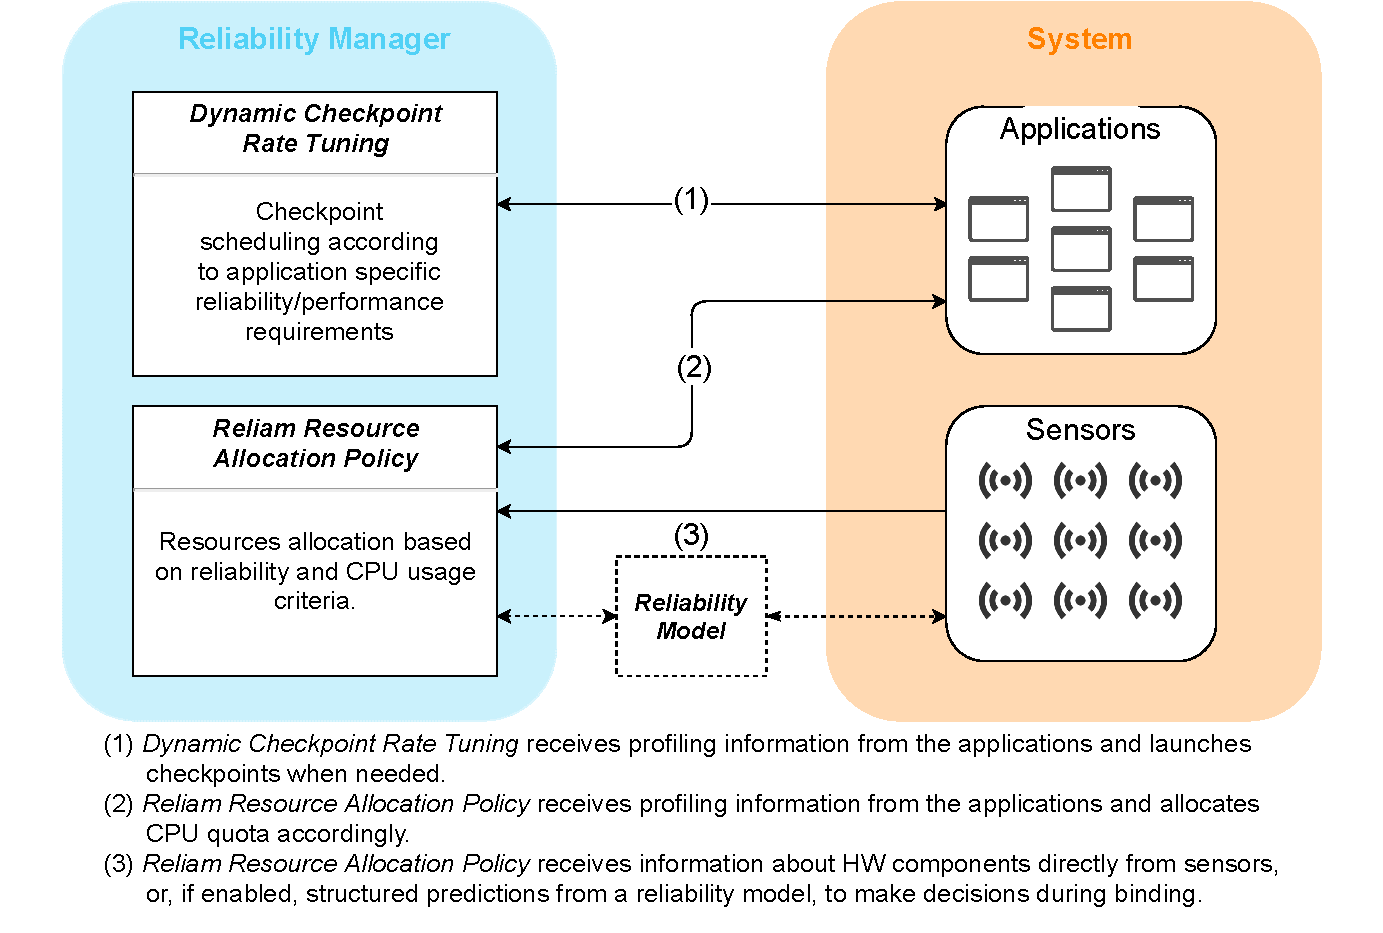
\includegraphics[width=\textwidth]{overview_thesis.pdf}
    \caption{Overview of the proposed work.}
    \label{fig:overviewth}
\end{figure}

The presented solution consists of two main components, the \emph{Dynamic Checkpoint Rate Tuning} and the \emph{Reliam Resource Allocation Policy}, which jointly contribute to achieve the above mentioned objective from different perspectives. An overview of the work, which will be deeply examined next in this chapter, is provided by Figure~\ref{fig:overviewth}.
The work proposed by this thesis is designed and implemented to be integrated both in the \emph{Barbeque Run-Time Resource Manager}, upon which an overview will be provided in the next paragraph.

\subsection{The Barbeque Run-Time Resource Manager}
\begin{figure}[t]
    \centering
    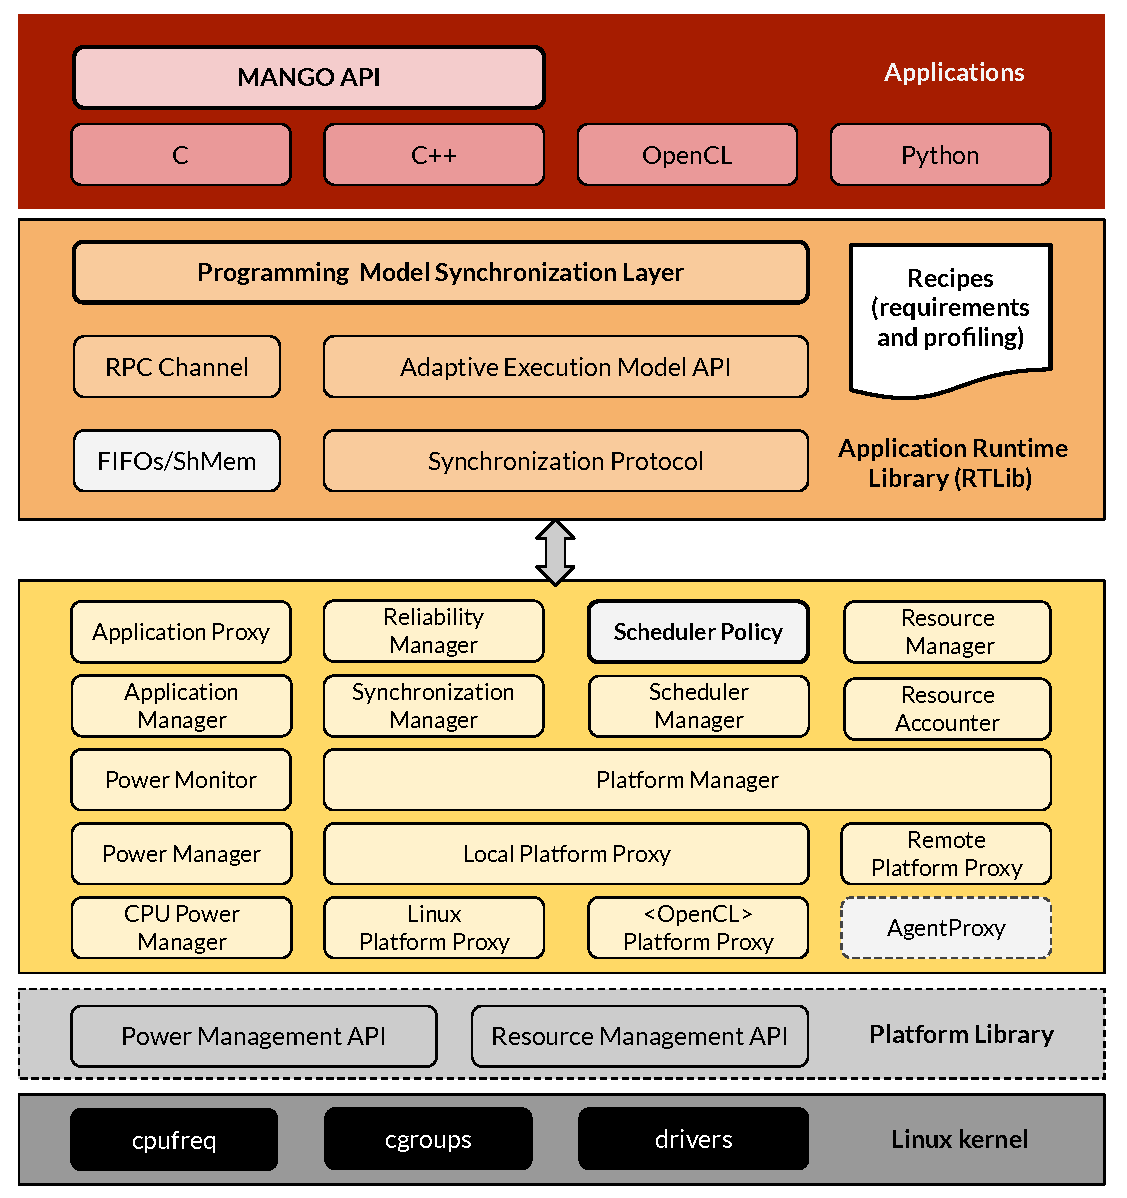
\includegraphics[width=0.8\textwidth]{bosp_architecture.pdf}
    \caption{Layer view of the BarbequeRTRM architecture.}
    \label{fig:bosp_arch}
\end{figure}
The Barbeque Run-Time Resource Manager (BarbequeRTRM) \cite{6322885} is a modular and extensible run-time resource manager that transparently manages the allocation of computing resources to multiple concurrent applications \cite{barbequertrm}. Its modular design facilitates the developer in the implementation and integration of resource allocation policies tailored to the need of each specific hardware configuration and use-case. As Figure~\ref{fig:bosp_arch} shows, the BarbequeRTRM is composed by various manager modules that provide the user with a wide range of information regarding applications, resources and optimization goals, which can be taken as input and tuned by the policy.
\begin{figure}[t]
    \centering
    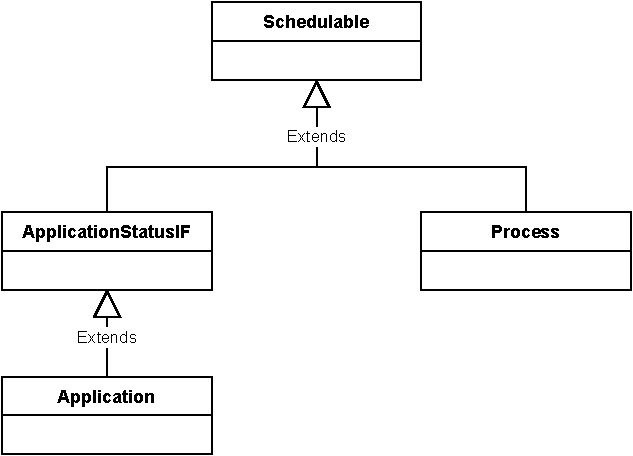
\includegraphics[width=0.8\textwidth]{uml_proc.pdf}
    \caption{Skeleton of the UML class diagram of the extensions of the class Schedulable in BarbequeRTRM.}
    \label{fig:umlproc}
\end{figure}

The framework is designed to manage the execution of generic processes, as well as integrated applications. This support is provided through the presence of a library called \verb|bbque_rtlib|, which defines a programming model called \emph{Adaptive Execution Model}, characterizing, the integrated applications. It consists in a managed execution flow in which application and Resource Manager communicate. Such interaction provides the application with a higher degree of awareness of the system, hence, the possibility to observe its own run time performance and throughput, as well as to adapt to the status of the hardware that it runs on. Conversely, it also enables the Resource Manager to assign resources taking into account the status of the system and the application requirements \cite{Zanella2019RunTimeMM}. 

The descriptors of both integrated and not-integrated applications are defined in the class \verb|Schedulable|, which stores any kind of information regarding the execution which it is instance of. Among other things, it keeps track of the process ID of the application, the state of the execution, the locality and the current resource assignment. On one hand, \verb|Schedulable| is extended by the abstract class \verb|ApplicationStatusIF| which defines an interface to query run-time information, inherited by the class \verb Application \, containing the descriptors of the integrated application. On the other hand, it is extended by the class \verb|Process|, defined to instantiate descriptors of generic processes. The above mentioned structure is shown in Figure~\ref{fig:umlproc}.

For the sake of simplicity, from now on, the terms \emph{application} and \emph{process} will be used interchangeably, since all of the features of this work have been designed and implemented for both types of workload.

\subsubsection{Hardware reliability support}
\label{sec:periodicchk}
The BarbequeRTRM is provided with a hardware reliability support based on a Periodic Checkpoint Mechanism, finalized by \emph{Checkpoint/Restore In Userspace (CRIU)}, a software tool running on Linux Operating System, as already mentioned in {\hyperref[sec:criu]{Section~\ref{sec:criu}}}. The checkpointing routine is initiated by the Reliability Manager. The function \verb|PeriodicCheckpointTask()| is called by a thread spawned at the launching of the platform and it periodically iterates over the running integrated application and managed processes, sequentially submitting them to the checkpointing procedure, without any kind of consideration of the status of the system and/or possible application requirements. To make this happen, the function \verb|Dump()| of the same module is called.  In this function, the interaction between the Reliability Manager and the Platform Manager modules takes place. Once the latter receives the checkpoint request from the former, it forwards it to the local or remote proxy able to carry out the dumping. In the case of the Local Platform Proxy, the implementations of the various \verb|Dump()| functions exposed by the Platform Proxy are called. Those proxy are, in fact, responsible of the actuation of the decisions made by the Resource Manager regarding each resource managed by the  BarbequeRTRM (CPU, NVIDIA GPU, custom accelerators, etc.) in the local node. Finally, CRIU provides to the deletion of the previous dump, if any, and to the generation of the current image, storing it in the directory specified in the configuration file of the framework.

Two limitations emerge from the current implementation:

\begin{description}
    \item [{\parbox[t]{\textwidth}{The checkpoint routine is completely unaware of the possible diversity of the running applications:}}] \hfill \\The only requirement which need to be to satisfied to proceed to the checkpointing routine is the expiration of the time period, without any kind of awareness regarding the time required by the checkpoint dump and, consequently, of the execution time left between two consecutive checkpoints of the same application. This mechanism is extended by the \emph{Dynamic Checkpoint Rate Tuning} component of this work in order to meet the reliability/performance requirements of each specific application.
    \item [{\parbox[t]{\textwidth}{The overwriting of the previous stored image results in costs in terms of reliability:}}]\hfill\\ In case of failure of the checkpoint procedure, not only the application pays the cost of the checkpoint overhead, but also has no backup until the next checkpoint, since the the previous image has been deleted. Moreover, it might happen that, even without the presence of such failure, the last checkpoint contains incorrect computation, due, for instance, to Silent Data Corruption. Also in this case, the possibility to restart from an earlier checkpoint might prevent the re-execution of all the application code. Also this weakness is taken into consideration by the proposed solution.
\end{description}

\section{Dynamic Checkpoint Rate Tuning}
\label{sec:dcrt}
The Dynamic Checkpoint Rate Tuning is one of the two main pillars of the proposed work. It takes place in the Reliability Manager module of the BarbequeRTRM and extends the already existing hardware reliability support, adding a level of application awareness to the Periodic Checkpoint Mechanism, analyzed in {\hyperref[sec:periodicchk]{Section~\ref{sec:periodicchk}}}.

\subsection{Design}
As previously anticipated, the simplicity of a periodic checkpointing algorithm is paid in terms of specificity with respect to the performance and reliability requirements of the considered application. In the case of a system in which more than one program is executing, it is reasonable to expect that, depending on the carried out functionality, each of them has different timing needs. For instance, one can think of a time critical application: if not properly tuned, the overhead produced by the checkpointing routine might cause a timing failure, an event that would highly compromise the delivered service. Conversely, in the case of a long-lasting execution application the need of a minimum overhead might be of secondary importance with respect to the need of a recent checkpoint to restart from in the event of a failure. The idea behind the Dynamic Checkpoint Rate Tuning is to adapt to both circumstances, providing the possibility to specify an upper bound on the checkpointing overhead, independently for each application. In BarbequeRTRM, this purpose is achieved by extending the Reliability Manager with a new task, carried out by the function \verb|DynamicCheckpointTask()|, called by a suitable thread at the launch of the platform, substituting the already existing \verb|PeriodicCheckpointTask()|. 

The above mentioned task must compute the following steps:
\begin{enumerate}[label={\arabic*)}]
    \item Select the next-in-list running application;
    \item Estimate the overhead that the checkpoint would bring to the execution if it were performed in that point in time;
    \item Compare the estimated overhead with the upper bound specified for the application;
    \item If the former is lower than the latter, the checkpointing routine is launched;
    \item Update checkpoint latencies of the application
    \item Go back to 1).
\end{enumerate}
As mentioned in {\hyperref[sec:periodicchk]{Section~\ref{sec:periodicchk}}}, from the reliability viewpoint, also the availability of only one saved image per time is a flaw of the current version of BarbequeRTRM: in the event of a failure in the dumping procedure, the running application is left without a useful checkpoint until the next dump is scheduled. To avoid the lack of reliability generated by this problem, a further modification has been introduced in the framework, in order to make it able to save more than one checkpoint. The extension proposed by this thesis work allows the possibility of specifying, in the configuration file, a destination folder in which a suitable number of consequent dumps are going to be stored, in order to improve the availability of a backup plan in the occurrence of failures during the execution of the application.

In the next paragraph, how the above mentioned changes have been implemented in BarbequeRTRM will be explained in details.

\subsection{Implementation}
\begin{figure}[t]
    \centering
    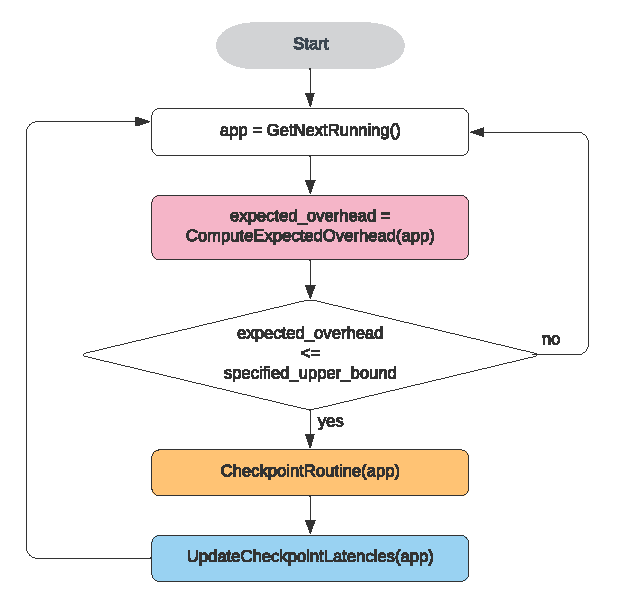
\includegraphics[width=0.6\textwidth]{dyn_chk_flow.pdf}
    \caption{Dynamic Checkpoint Rate Tuning algorithm.}
    \label{fig:dynchk}
\end{figure}
The steps followed by the Dynamic Checkpoint Rate Tuning algorithm, implemented in the function \verb DynamicCheckpointTask() \ of the Reliability Manager module, are summarized in the flowchart in Figure~\ref{fig:dynchk}, whose main basic blocks are going to be analyzed in the following sections.

\subsubsection{Computation of the expected overhead}

Given a running application, the first step of the algorithm is to compute the expected overhead a checkpoint would bring to the execution at that given point in time. 

The estimate of the checkpoint latency is given by the arithmetic mean of the previous completed dumps, stored as an attribute of the class \verb Schedulable . For each invocation of the algorithm, the expected overhead is computed considering the ratio between the cumulative amount of time spent performing checkpoints and the total time elapsed since the start of the application, in order to diminish the impact of the variance on the overhead. More specifically, the followed procedure is presented in pseudo code in Algorithm~\ref{alg:chk_overhead}.
\begin{algorithm}
    \SetKwInput{KwInput}{Input}                % Set the Input
    \SetKwInput{KwOutput}{Output}              % set the Output
    \DontPrintSemicolon
    \BlankLine
    \KwInput{Application descriptor \emph{app}}
    \KwOutput{Estimated checkpoint overhead}
    %\BlankLine
    \algrule
% Set Function Names
    \SetKwFunction{Func}{ComputeExpectedCheckpointOverhead}
% Write Function with word ``Def''
  \SetKwProg{Fn}{Def}{:}{}
  \Fn{\Func{$app$}}{
  \BlankLine
        mean\_chk\_time = app$\rightarrow$GetCheckpointLatencyMean()\;
        elapsed\_time = app$\rightarrow$GetElapsedTimeSinceStart()\;
        total\_time = elapsed\_time + expected\_chk\_time\;
        nr\_completed\_chk = app$\rightarrow$GetNrPerformedCheckpoints()\;
        sum\_chk\_time = (nr\_completed\_chk +1) * mean\_chk\_time\;
        expected\_chk\_overhead = sum\_chk\_time/total\_time\;}
        \BlankLine
        \KwRet expected\_chk\_overhead\;
    \BlankLine
   \caption{Estimation of checkpoint overhead algorithm.}
   \label{alg:chk_overhead}
\end{algorithm}


\subsubsection{Checkpoint Routine and Checkpoint Latencies Updating}
\label{sec:chkroutine}
Once computed the expected checkpoint overhead, it must be compared to the upper bound specified for considered application: if the former is not greater than the latter, the checkpoint routine starts. The control flow of the checkpoint routine is summarized in Figure~\ref{fig:chk_routine}. 

\begin{figure}[t]
    \centering
    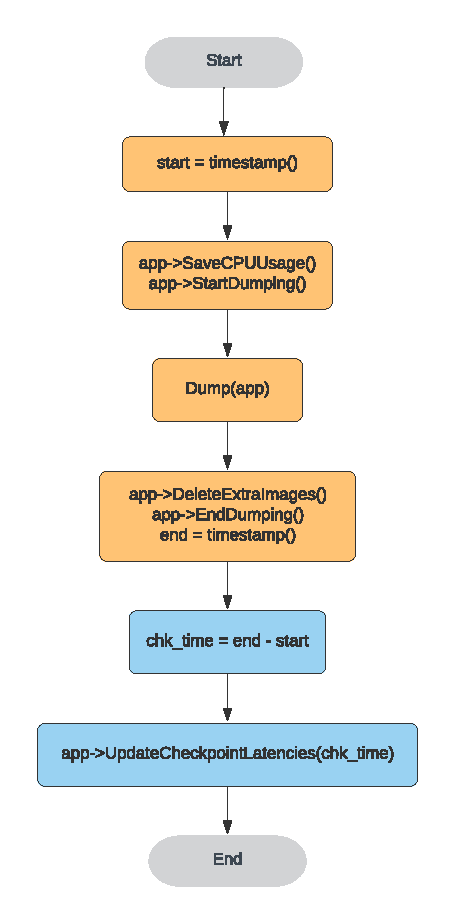
\includegraphics[width=0.5\textwidth]{chk_routine.pdf}
    \caption{Checkpoint Routine and Checkpoint Latencies Updating flowchart.}
    \label{fig:chk_routine}
\end{figure}
As a first step, the present timestamp is stored in order to keep track of the duration of the procedure. Secondarily, the current CPU usage of the application is stored and the application Boolean attribute \verb is_dumping \ is set through the member function \verb StartDumping() \footnote{A definition of \emph{CPU usage} and the motivations behind the need of this basic block will be provided in {\hyperref[sec:reliam]{Section~\ref{sec:reliam}}}.}.

After these preliminary steps, the generation of the image is performed as it was in the already existent hardware reliability support (see {\hyperref[sec:periodicchk]{Section~\ref{sec:periodicchk}}}). Differently from before, in this procedure, the deletion of the previous generated images takes place only if the number of currently saved dumps exceeds the one specified in the configuration of the framework.

The last step of the checkpoint routine is to reset the Boolean attribute of the application \verb is_dumping \ and to catch the ending timestamp.

Finally, the checkpoint latencies of the application are updated.

\section{Reliam Resource Allocation Policy}
\label{sec:reliam}
In the previous section, we discussed about the Dynamic Checkpoint Rate Tuning, the first component of this work, this section will, instead, focus on the Reliam Resource Allocation Policy. While the former was designed and implemented as a fault tolerance mechanism, i.e. to properly \emph{react} to an already occurred failure, in order to minimize its impact on the system, the latter has been conceived to \emph{proactively} improve the reliability of the hardware components.

\begin{figure}[t]
    \centering
    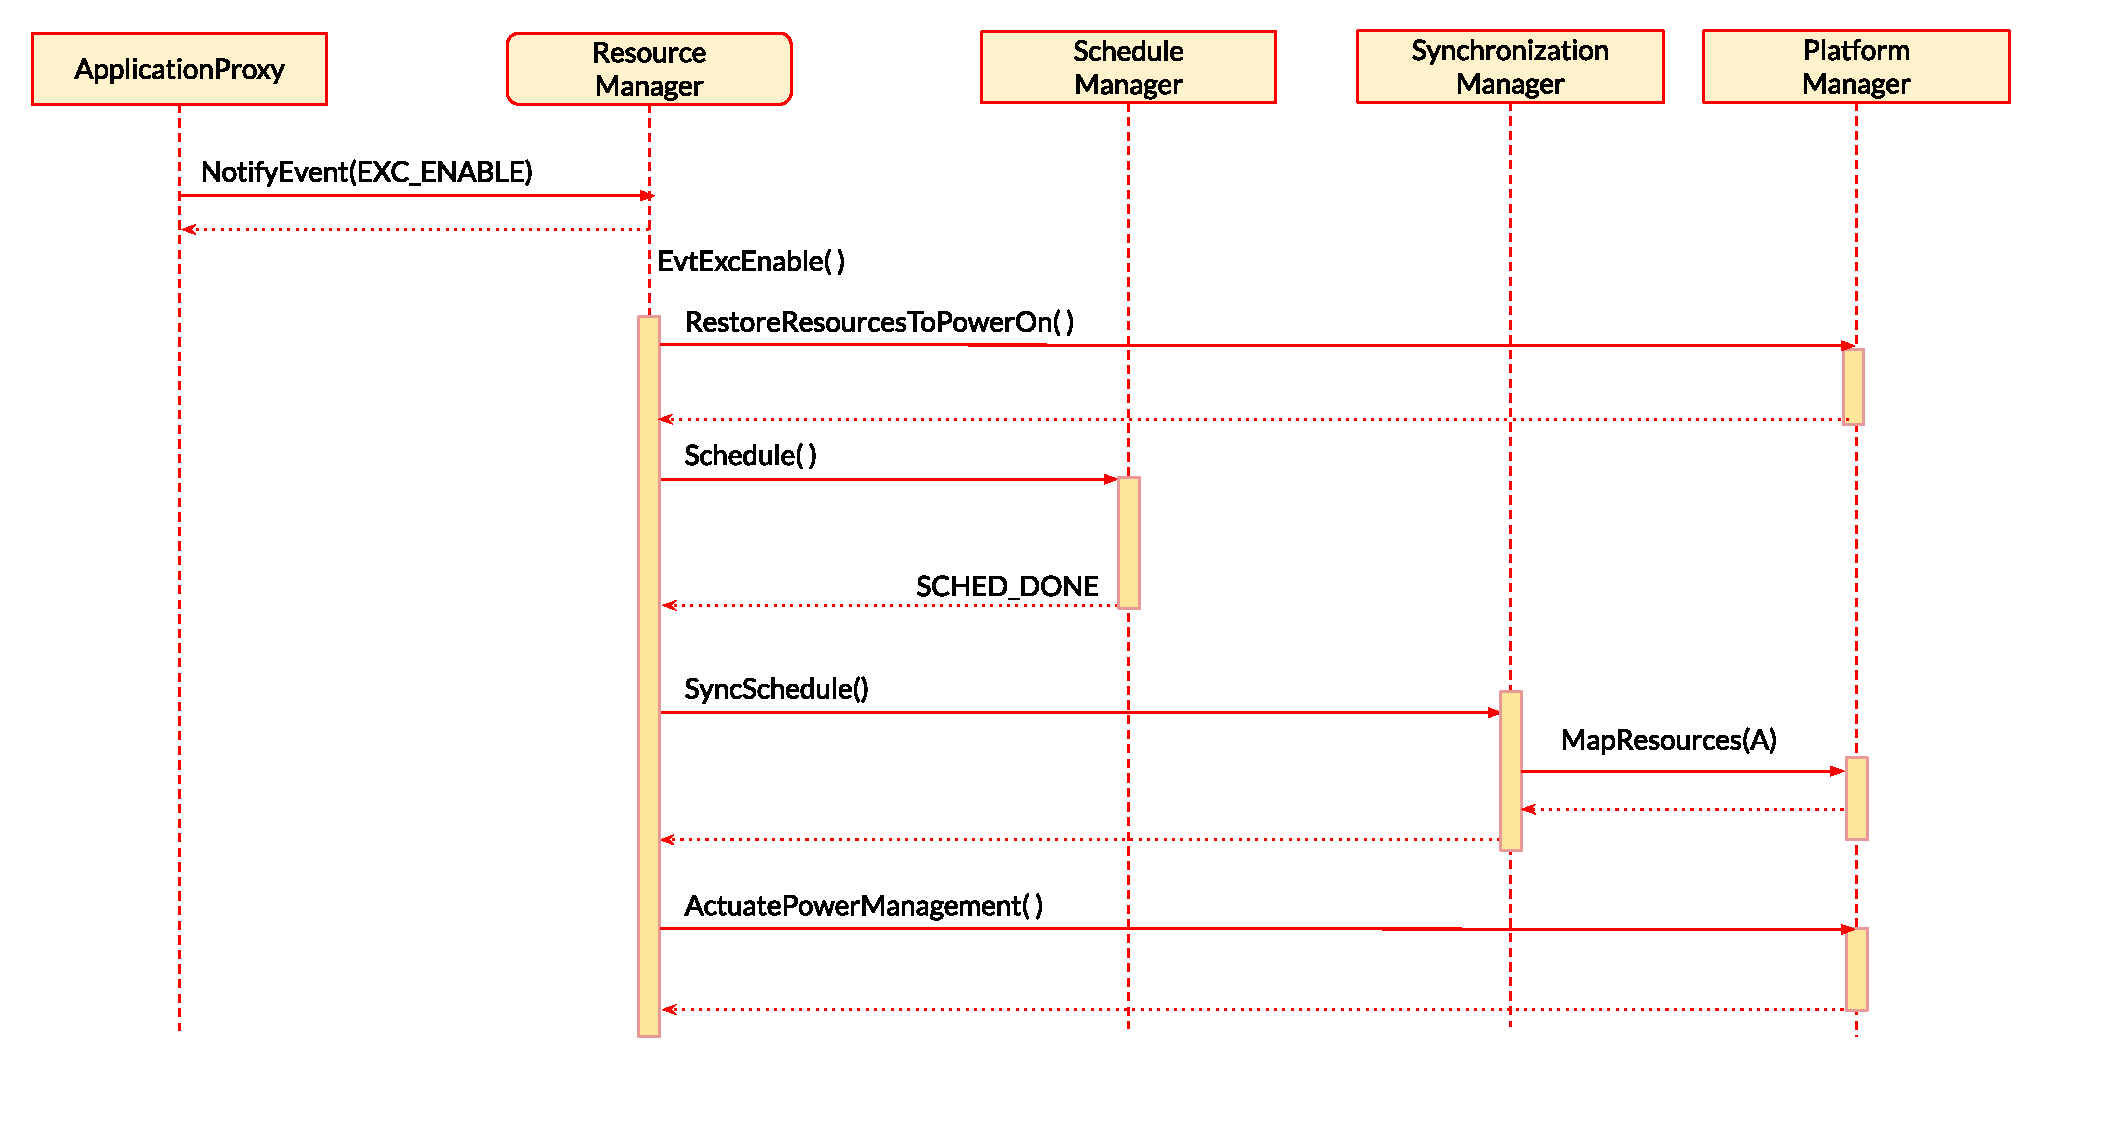
\includegraphics[width=0.95\textwidth]{bosp_flow.pdf}
    \caption{Resource assignment flow of the BarbequeRTRM.}
    \label{fig:bosp_flow}
\end{figure}

The purpose of the Reliam Resource Allocation Policy is to assign computational resources minimizing CPU usage and aging, and it is integrated as a plugin of the BarbequeRTRM.
Figure~\ref{fig:bosp_flow} summarizes the resource assignment flow of the above mentioned framework, focusing on the interaction between the main modules involved in the implementation of a generic resource allocation policy: the component discussed in this Section lies in the scheduling management part and its entry point correspond to the function \verb|Schedule()|. This function starts the execution of the allocation policy specified in the configuration phase, whose plugin is loaded when the Resource Manager is launched.

\subsection{Design}
\label{sec:poldesign}
Reliam is a resource allocation policy that must be launched on a periodical basis, whose main objective is to prevent the wear out of the computing resources and, consequently, to slow down their aging. Aside from the reliability matter, we designed a modified version of Proportional Integral Derivative (PID) controller and we implemented it to adapt the CPU quota allocation to the need of each application. This approach allowed us to reach the minimization of the CPU utilization and, consequently, better global performances, especially in the case of parallel executions. Before going into the details of the design, some definition will be firstly provided in order to guarantee the necessary background of knowledge for the reader.

\begin{description}
\item[CPU quota.]
CPU \emph{quota} is defined as the percentage, in terms of time, of CPU resources (available or allocated) where the total amount is expressed as:
\[total\_cpu\_quota = total\_nr\_cpu\_cores * 100\]
\item[CPU usage.]
Given a resource allocation to an application, we define as CPU \emph{usage} the CPU quota effectively exploited during the execution. For each application, CPU usage never exceeds the allocated CPU quota.
\item[PID controller.]
\begin{figure}[t]
    \centering
    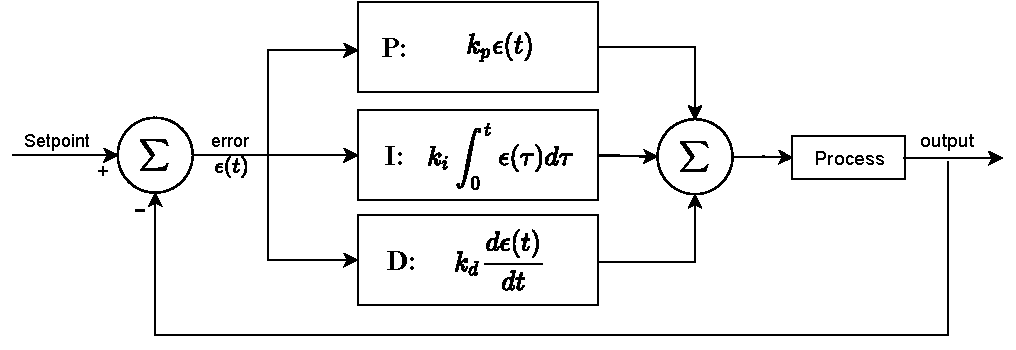
\includegraphics[width=\textwidth]{pid.pdf}
    \caption{PID controller block diagram.}
    \label{fig:pid}
\end{figure}
A PID controller is a control loop mechanism employing feedback to make the output converge to a set point, using Proportional, Integral and Derivative contributions weighted by coefficients, respectively $k_{p}$, $k_{i}$ and $k_{d}$, as shown by the block diagram in Figure~\ref{fig:pid}.

\item[Dark Silicon.]
With the end of Dennard scaling, as well as single-core scaling, also multi-core scaling is going to be constrained, due to the power limitations of the future designs, which will reduce the usable chip fraction \cite{10.1145/2024723.2000108}.
\emph{Dark Silicon} is the practice of turning off a number of cores in a chip in order to satisfy energy and thermal constraints. 
\item[Process Freezing.]
Process \emph{freezing} is a temporary and controllable pause state in the execution of a process, which will be able to resume its work after being \emph{thawed}.
\item[Process Thawing.] 
We define as process \emph{thawing} the reverse operation of freezing, after which an application is able to resume its execution.
\end{description}
\begin{figure}[t]
    \centering
    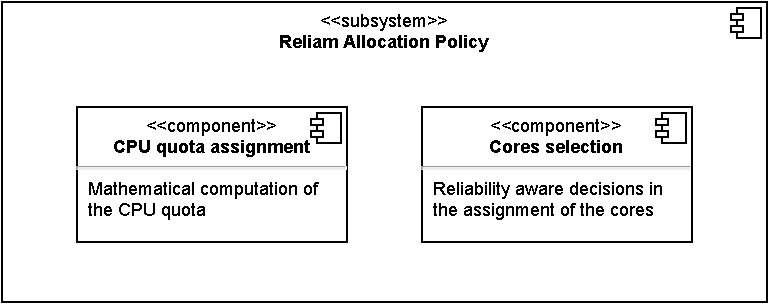
\includegraphics[width=0.8\textwidth]{comp_reliam.pdf}
    \caption{Reliam Resource Allocation Policy design components.}
    \label{fig:reliam_design}
\end{figure}

Reliam Resource Allocation Policy assigns to each application a modified version of a PID controller, in order to periodically compute the CPU quota to allocate, such that, at each invocation, it will be closer to the effective CPU usage of the application at issue. Once all CPU quotas are defined, the selection of the cores, based upon reliability criteria, is performed. The main components of the design of the policy are summarized in Figure~\ref{fig:reliam_design} and will be analyzed in depth in the next paragraphs.

\subsubsection{Computation of the CPU quota}
To better understand the rationale behind the logic of Reliam Allocation Policy 
We ideally define the PID controller variables as follows:
\begin{enumerate}[label=-]
    \item Control variable: $cv$
    \item Process variable: $\Delta$
    \item Setpoint: $\overline{\Delta}$
    \item Error: $\epsilon$
\end{enumerate}
such that:
\begin{enumerate}[label=]
    \item $cv = k_{p}*\epsilon_r + k_{i}*\sum_{k\in R}\epsilon_{k} + k_d*(\epsilon_{r}-\epsilon_{r-1})$
    \item $\Delta = CPU_{A} - CPU_{U}$
    \item $\epsilon_r = \overline{\Delta} - \Delta$
\end{enumerate}
where, considering numbered invocations of the policy, $\epsilon_r$ is the error observed at invocation $r$, while $CPU_{A}$ and $CPU_{U}$ are, respectively, the CPU quota assigned and the CPU usage of the application.

In the proposed work, we brought one fundamental change to the PID controller model in order to better fit the adaptive resource allocation problem. We decided to set to zero integral and derivative contributions in the case of \(\epsilon(t)=0\), i.e. every time the output matches the set point, avoiding pointless fluctuations of the control variable.
Considering this change in the computation of the control variable, the final ideal model is defined as follows:

\begin{flalign*}
    \renewcommand{\arraystretch}{3}
    \begin{array}{ll}
        cv &= 
            \begin{cases}
        	    k_{p}*\epsilon_r + k_{i}*\sum_{k\in R}\epsilon_{k} + k_d*(\epsilon_{r}-\epsilon_{r-1}) & \mbox{if } \epsilon\neq 0 \\
        	    0 & \mbox{otherwise}
    	    \end{cases}\\
        \Delta &= CPU_{A} - CPU_{U} \\
    	\epsilon_r &= \overline{\Delta} - \Delta
	\end{array}
\end{flalign*}

Once defined the ideal model, we need to introduce slight changes to the process variable $\Delta$ and the computation of the error $\epsilon$ for the sake of the applicability in a real scenario.

\begin{description}
\item[Process variable: $\Delta$.]
Consider the $r^{th}$ invocation of the policy with $r>1$.
Given a CPU quota allocation to an application, if, in the previous invocation, the CPU quota has exceeded the observed CPU usage, it is reasonable to infer that a lesser assignment can be performed. The process variable $\Delta$ is computed as:
\begin{align*}
    \Delta = CPU_{A} - CPU_{U}
\end{align*}
Conversely, $CPU_{A} == CPU_{U}$ means that the application saturated all the assigned resources, thus it might use more of them if available. As already mentioned, the following inequality always applies: 
\begin{align*}
    CPU_{U} \leq CPU_{A}
\end{align*}
Since, in this scenario, we are not able to infer the CPU usage the application would have shown if a larger CPU quota had been assigned to it, we assign to $\Delta$ a negative constant:
\begin{align*}
    \Delta = \Delta_{NEG}
\end{align*}
This modification to the ideal $\Delta$ allows us to a more balanced use of the controller, which, otherwise, would have properly worked only with positive values of $\Delta$.
\item[Error: $\epsilon$.]
\begin{figure}[t]
    \centering
    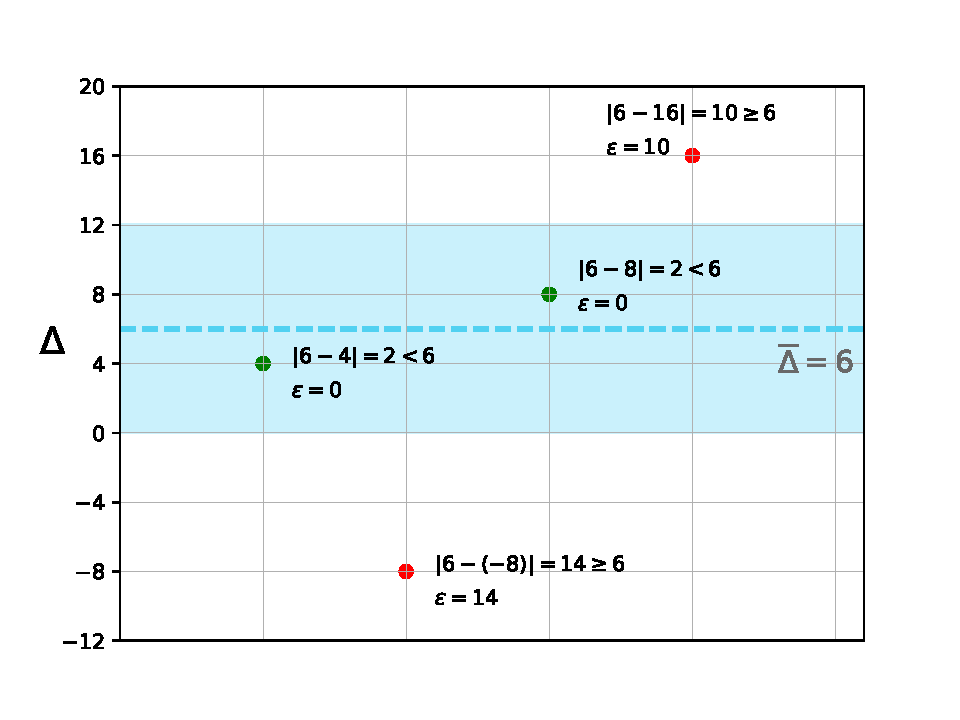
\includegraphics[width=0.8\textwidth]{delta.pdf}\vspace{-1.15em}
    \caption{Graphical explanation of the computation of the error in the real model of the modified PID Controller. The blue area corresponds to the values of $\Delta$ such that $\epsilon=0$.}
    \label{fig:delta}
\end{figure}
During its execution, it is reasonable that an application maintains the same CPU usage, net of some small variation. In order to avoid a new computation of the quota if, in two consecutive invocations, the observed CPU usage is similar but not equal, we relaxed the computation of $\epsilon$ in order to be 0 if $\Delta$ is \emph{close enough} to $\overline{\Delta}$, such that if:
\begin{flalign*}
    |\overline{\Delta}-\Delta| \leq \overline{\Delta}
\end{flalign*}
given that:
\begin{flalign*}
    |\overline{\Delta}-\Delta_{NEG}| \geq \overline{\Delta} 
\end{flalign*}
the error $\epsilon$ remains equal to zero.
\end{description}
Changes above considered, we can finally define the real model as:
\begin{enumerate}[label=-]
    \item Control variable: $cv$
    \item Process variable: $\Delta$
    \item Setpoint: $\overline{\Delta}$
    \item Error: $\epsilon$
\end{enumerate}
where:
\begin{align*}
    \renewcommand{\arraystretch}{3}
    \begin{array}{ll}
        cv &= 
        \begin{cases}
                k_{p}*\epsilon_r + k_{i}*\sum_{k\in R}\epsilon_{k} + k_d*(\epsilon_{r}-\epsilon_{r-1}) & \qquad \mbox{if } \epsilon\neq 0 \\
        	    0 & \qquad\mbox{otherwise} 
        \end{cases}\\
        \Delta &= 
            \begin{cases}
        	    CPU_{A} - CPU_{U} \hfill& \qquad \mbox{if } CPU_{A} > CPU_{U} \\
        	    \Delta_{NEG} &\qquad \text{otherwise}
    	    \end{cases}\\
    	    \epsilon &=
    	    \begin{cases}
        	    \overline{\Delta} - \Delta &\qquad\mbox{if } |\overline{\Delta}-\Delta| \geq \overline{\Delta}\mbox{}\\
        	    0 &\qquad \mbox{otherwise}
    	    \end{cases}
	\end{array}
\end{align*}


A graphical explanation of the computation of the error is provided in Figure~\ref{fig:delta}. In the example, $\overline{\Delta}=6$, hence, the values of $\Delta$ marked in green produce $\epsilon=0$, while $\epsilon=\overline{\Delta}-\Delta$ for the ones colored in red.

\subsubsection{CPU cores selection and reliability monitor}
\label{sec:corsel}
In the previous paragraph, we defined the model used to compute the CPU quota assigned by the policy to the applications, in this one, we will provide details about the selection of the processing elements that are supposed to provide such CPU quota.

The idea behind the designed selection mechanism is to emulate at software level the effect of Dark Silicon, in order to keep the temperature of the system components in a safe operating range. The above mentioned goal is achieved allocating the CPU cores in a sequential fashion\cprotect\footnote{BarbequeRTRM provides two policies of CPU quota partitioning:
\begin{itemize}
    \item SEQUENTIAL: a new core is bound to the application only if all the CPU quota associated to the previous one has been allocated;
    \item BALANCED: each available core equally contributes to the handling of the request.
\end{itemize}}, i.e. saturating the quota of each bound core, in ascending order of temperature, before allocating a new one. In this way we obtain that, in the case in which not all computational resources available in the system are needed, warmer cores are the ones that remain idled. Moreover, in all circumstances, all the processing elements exceeding their safety critical temperature are forced to idle. The policy is also entrusted with the ability of freezing applications classified as \emph{critical} with respect to the reliability of the system. More specifically, an application will be frozen if all the processing element bound to it with quota 100 are exceeding their safety critical temperature. In this way, the idling of those cores will impact only on the performance of that specific application and not on the entire system. Since, at the time of writing, modern Intel CPUs apply \emph{Dynamic Voltage and Frequency Scaling (DVFS)} at hardware/firmware level, we do not have the possibility to directly resort to such technique at software level. Nonetheless, its contribution is transparently added to the effectiveness of our solution by the design of the processing units.

Furthermore, the flexibility of the policy allows the possibility to consider more than one reliability input. Core temperature measurement can be combined with more comprehensive reliability profiling data, if compatible monitoring tools or interfaces are integrated with the Reliam Resource Allocation Policy. At the time of writing, BarbequeRTRM is provided with a library called \verb|libhwrel| \cite{recipedel} which consists of a hardware reliability monitor able to predict the degradation of their reliability. It is composed by three main classes: \verb|Request|, which contains the requests sent by the Resource Manager to the library, \verb|Response| which contains the response to such requests, and the main class \verb|HWReliabilityMonitor| which performs the actual analysis, taking a \verb|Request| object as an input and providing a \verb|Response| object as an output. In the requests, it is possible to specify the resource type (CPU, GPU, Memory, etc.) and the technology used (ASIC, FPGA, etc.): after appropriate analysis, the library will output a number representing the probability of failure in per-mille/program-run \cite{recipedel}. If \verb|libhwrel| is linked to the policy, the ordering of the cores will be made in ascending order of their \verb|Response| output of the \verb|libhwrel|.

For the sake of generality, in the following section, the basic implementation, extracting the temperature values directly through the sensors output, will be examined.

\subsection{Implementation}
\begin{figure}[t]
    \centering
    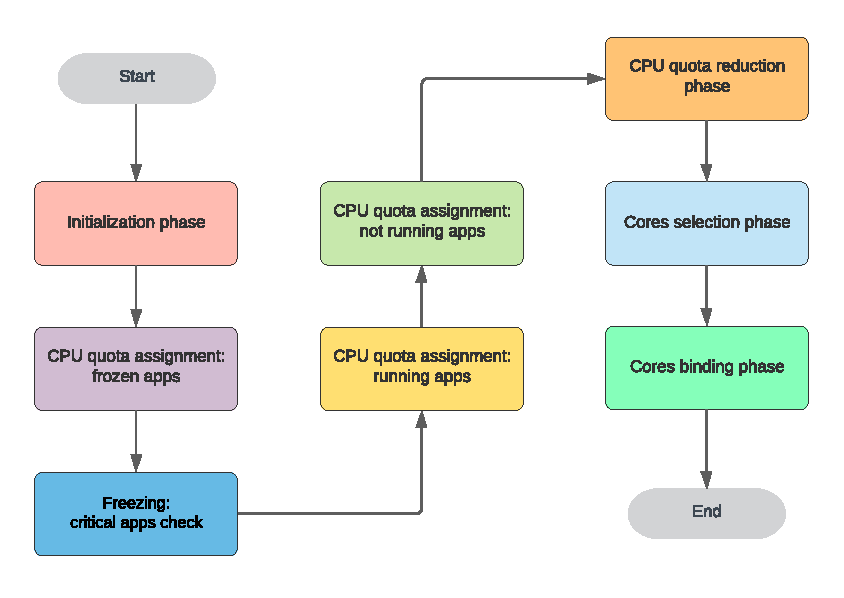
\includegraphics[width=\textwidth]{policy_flow.pdf}
    \caption{Control flow of the Reliam Resource Allocation Policy.}
    \label{fig:policyflow}
\end{figure}

Reliam Resource Allocation Policy has been implemented in the BarbequeRTRM following the sequential control flow shown in Figure~\ref{fig:policyflow}. All blocks will be independently examined in the following paragraphs, since the sequential structure of the policy allows an easily done partitioning in basic blocks. 

Before examining in depth the implementation of the policy some preliminary information is provided:
\begin{itemize}
\item The map \verb|assigned_quotas|, having as key the application descriptor descriptor and as value the its computed CPU quota is instantiated as an attribute of the class: every time a CPU quota is computed, an element is added to the map;
\item Given an application, it is always possible to retrieve its last assigned CPU quota: in this thesis, for the sake of simplicity, it will be always done through the use of the function \verb|GetPrevQuota()|;
\item Given an application, it is always possible to retrieve its CPU usage \emph{respective to the last point in time in which it was executing}: in this thesis, for the sake of simplicity, it will be always done through the use of the function \verb|GetCPUUsage()|. Considering, for instance, a resource allocation taking place right after the performing of a checkpoint, such function will return the CPU usage of the moment right before the suspension of the execution.
\item In this paper we will refer to the CPU quota assigned in the current invocation of the policy as \emph{next\_quota}, while \emph{prev\_quota} will refer to the CPU quota assigned in the invocation right before the current one.
\end{itemize}
\begin{figure}[t]
    \centering
    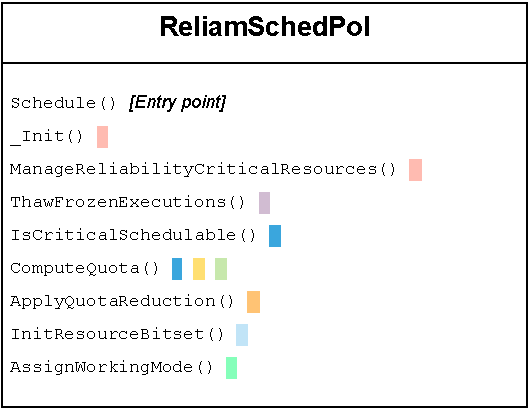
\includegraphics[width=0.6\textwidth]{reliam_uml.pdf}
    \cprotect\caption{Partial UML class diagram of the class \verb|ReliamSchedPol|.}
    \label{fig:reliamuml}
\end{figure}

In Figure~\ref{fig:reliamuml},  a partial UML class diagram of class  \verb|ReliamSchedPol|, implementing the Reliam Resource Allocation Policy, is shown: the main member functions are listed, next to the colors of the basic blocks of the flowchart in Figure~\ref{fig:policyflow} that they implement.

\subsubsection{Initialization phase}
\label{sec:init}
The initialization phase takes place in the member functions \verb _Init() \ and \verb|ManageReliabilityCriticalResources()|, directly called by \verb|Schedule()|, the entry function of the policy. During initialization, the definition of the main inputs of the policy takes place. In order to ensure the functioning of the design described in the previous section, the following attributes are initialized:

\newcommand\vitem[1][]{\SaveVerb[%
    aftersave={\item[\textnormal{\UseVerb[#1]{vsave}}]}]{vsave}}
\begin{description}
    \vitem +nr_not_running_apps:+ the number of managed applications not scheduled yet. This information is directly provided by the Application and Process Manager modules of the framework.
    \vitem +id_cpu_cores_to_idle:+ list of the id of CPU cores that are going to be forced to idle by the policy, for reliability reasons. This information is computed comparing the critical temperature of each core against the current one. Both pieces of information are fetched through the Power Manager module. 
    \vitem +nr_cpu_cores_to_idle:+ the number of CPU cores to set to idle mode for reliability reasons. It is the size of the list defined in the previous attribute.
    \vitem +nr_cpu_cores_prev_idle:+ the number of CPU cores forced to idle mode for reliability reasons in the previous invocation of the policy. Such information it is stored by the policy in the Reliability Manager at each invocation.
    \vitem +nr_cpu_cores_resumed_from_idle:+ difference in the number of cores idled between the previous and the current invocation, i.e. \verb nr_cpu_cores_prev_idle \ - \verb|nr_cpu_cores_to_idle|. 
    \vitem +available_cpu_cores:+ list containing the descriptors of all the CPU cores available in the system.
    \vitem +available_cpu_quota:+ the total CPU quota allocatable by the policy, net of the amount corresponding to the cores that are going to be idled in the current invocation. Given the number of cores available in the system \verb total_nr_cpu_cores , it is computed as:  \verb (total_nr_cpu_cores \ - \verb|nr_cpu_cores_to_idle)*100|. Every time a CPU quota is assigned to application, this variable will be decremented by such assignment to keep track of the residual availability.
\end{description}
Once all of the necessary information has been retrieved, the actual computation takes place.

\subsubsection{CPU quota assignment: frozen applications}
As mentioned in the design of the \emph{cores selection} component, it is possible for the policy to freeze a \emph{critical} application, for reliability reasons (details will be provided in the next paragraph). As a consequence of this feature, at each invocation, right after the initialization phase, the first step of the policy results in checking the necessary condition to thaw frozen executions, if any. 

\verb nr_cpu_cores_resumed_from_idle \ > 0 is the necessary condition to start the thawing process and it is checked in the member function  \verb|ThawFrozenExecutions()|.

More specifically, the policy iterates over the frozen applications, thawing them and assigning as much CPU quota as possible, considering as upper bound the smaller value between the last CPU quota assigned before it was frozen and \verb|nr_cpu_cores_resumed_from_idle*100|.
Algorithm~\ref{alg:thaw} shows the exact procedure followed by the first computational step of the policy. 
\begin{algorithm}[t]
    \SetKwInput{KwInput}{Input}                % Set the Input
    \SetKwInput{KwOutput}{Output}              % set the Output
    \DontPrintSemicolon
    \BlankLine
    \KwInput{\FuncSty{available\_cpu\_quota, nr\_cpu\_cores\_resumed\_from\_idle}}
 %   \KwInput{\FuncSty{nr\_cpu\_cores\_resumed\_from\_idle}}
    \KwOutput{None}
    %\BlankLine
    \algrule
% Set Function Names
    \SetKwFunction{Func}{ThawFrozenExecutions}
% Write Function with word ``Def''
  \SetKwProg{Fn}{Def}{:}{}
  \Fn{\Func{available\_cpu\_quota,  nr\_cpu\_cores\_resumed\_from\_idle}}{
  \BlankLine
        resumed\_cores = nr\_cpu\_cores\_resumed\_from\_idle\; 
        \While{resumed\_cores > 0}
        {
            app = GetNextFrozen()\;
            prev\_quota = app$\rightarrow$GetPrevQuota()\tcp*[r]{last quota}
            \eIf{prev\_quota/100 > resumed\_quota}
            {
                 assigned\_quotas[app] = resumed\_cores*100\;
                 resumed\_cores = 0 \;
            }{
                assigned\_quotas[app] = prev\_quota\;
                resumed\_cores -= prev\_quota/100\;
            }
            available\_cpu\_quota -= assigned\_quotas[app]\;
            Thaw(app)\;
        }
    }
        \BlankLine
    \BlankLine
   \caption{Process Thawing algorithm.}
   \label{alg:thaw}
\end{algorithm}


\subsubsection{Freezing: critical applications check}
As already anticipated, the policy has been provided with the capability of freezing an application in the case it has been acknowledged as \emph{critical}. More specifically, we classify as critical each application such that, after the initialization phase, the list \verb|id_cpu_cores_to_idle| contains as elements \emph{all} the IDs of the CPU cores assigned to such application \emph{with CPU quota equal to 100}. The check at issue and is carried out by the boolean member function \verb|IsCriticalSchedulable()|, called by \verb|ComputeQuota()|. If the return value is \verb true , the latter takes care of saving the amount of the lastly assigned CPU quota, in order ensure its retrieval, in later invocations of the policy, by the procedure described in the previous paragraph. The control flow of this entire algorithm can be found in Figure~\ref{fig:freeze}.
\begin{figure}[t]
    \centering
    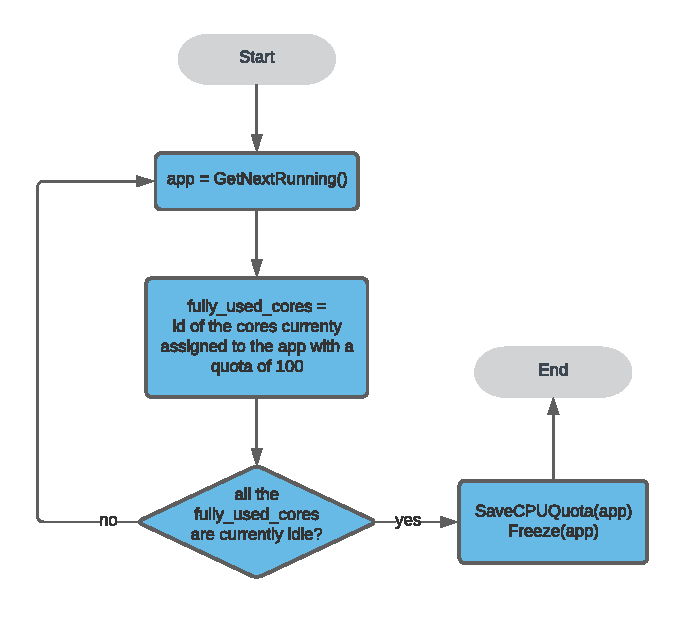
\includegraphics[width=0.9\textwidth]{check_to_freeze.pdf}
    \caption{Critical applications check.}
    \label{fig:freeze}
\end{figure}

\subsubsection{CPU quota assignment: running applications}
The basic block concerning the computation of the CPU quota to allocate for running application represents the core of the policy and consists in the implementation of the model described in the {\hyperref[sec:poldesign]{Design Section}}. The control flow of this component, for each application at issue, is described by Figure~\ref{fig:runapp}. 
\begin{figure}[t]
    \centering
    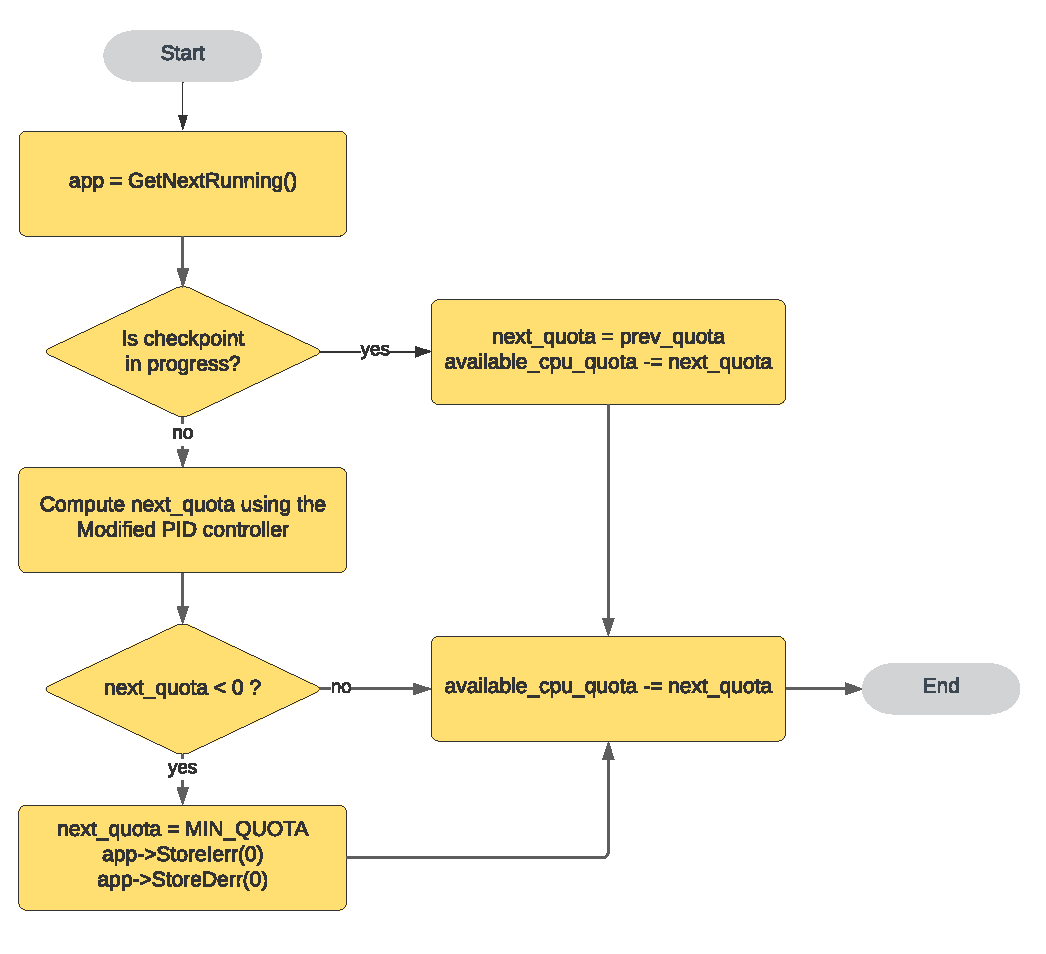
\includegraphics[width=0.8\textwidth]{running_apps.pdf}
    \caption{CPU quota assignment for running app control flow.}
    \label{fig:runapp}
\end{figure}

As shown in the above mentioned flowchart, the first step of the procedure is checking if a checkpointing of the application at issue is taking place. This check is possible thanks to the setting of the Boolean attribute of the application \verb is_dumping , carried out by the checkpointing routine previously considered in this work\footnote{See paragraph {\hyperref[sec:chkroutine]{\emph{Checkpoint Routine and Checkpoint Latencies Updating}}} of this chapter.}. If such attribute is set, i.e. the checkpointing is in progress, the policy will allocate for the application the same CPU quota lastly assigned.
Conversely, if the application is regularly executing, the Modified PID controller will compute the new CPU quota to assign. Algorithm~\ref{alg:pid} shows the pseudo-code of the procedure followed by the controller, implementing the model previously designed in this Section.

\begin{algorithm}
    \SetKwInput{KwInput}{Input}  
    \SetKwInput{KwConstant}{Constant}% Set the Input
    \SetKwInput{KwOutput}{Output}              % set the Output
    \DontPrintSemicolon
    \BlankLine
    \KwInput{Application~descriptor:~\emph{app}}
    \KwOutput{Assigned CPU quota: \emph{next\_quota}}
    \KwConstant{\ArgSty{ADMISSIBLE\_DELTA, NEG\_DELTA, Kp, Ki, Kd}}
    %\BlankLine
    \algrule
% Set Function Names
% Write Function with word ``Def''
 \nonl\emph{Modified PID Controller:}\;
\BlankLine
  {
    prev\_quota = app$\rightarrow$GetPrevQuota()\;
    cpu\_usage = app$\rightarrow$GetCPUUsage()\;
    delta = prev\_quota - cpu\_usage\;
    error = ADMISSIBLE\_DELTA/2 - delta\;
    
   
    \uIf{delta == 0 \tcp*[r]{all assigned resources have been used}}
    {
        delta = \ArgSty{NEG\_DELTA}
    }
    
    \ElseIf{ (abs(error) < ADMISSIBLE\_DELTA/2)}
        {error = 0\tcp*[r]{admissible range}
        app$\rightarrow$StoreIerr(0)\;
        app$\rightarrow$StoreDerr(0)\;}
    
    pvar = Kp*error\tcp*[r]{PROPORTIONAL CONTROLLER}

    
    ierr = error + app$\rightarrow$ierr\;
    app$\rightarrow$StoreIerr(ierr)\;
    ivar = Ki*ierr\tcp*[r]{INTEGRAL CONTROLLER}
    
   
    derr = error - app$\rightarrow$derr\; 
     app$\rightarrow$StoreDerr(derr)\;
    dvar = Kd*derr \tcp*[r]{DERIVATIVE CONTROLLER}

    cv = pvar + ivar + dvar\tcp*[r]{control variable}
    
     next\_quota = prev\_quota + cv\tcp*[r]{assigned quota}
     \KwRet{next\_quota}
  \BlankLine
        
    }
        \BlankLine
    \BlankLine
   \caption{Modified PID controller algorithm.}
   \label{alg:pid}
\end{algorithm}

Since the model is blind with respect to the fact that the allocated CPU quota must be greater than zero, a last check is needed: if the above mentioned condition is not satisfied, a \emph{minimum default value} will be allocated and the Integral and Derivative contributions reset.

\subsubsection{CPU quota assignment: not running applications}
\begin{figure}[t]
    \centering
    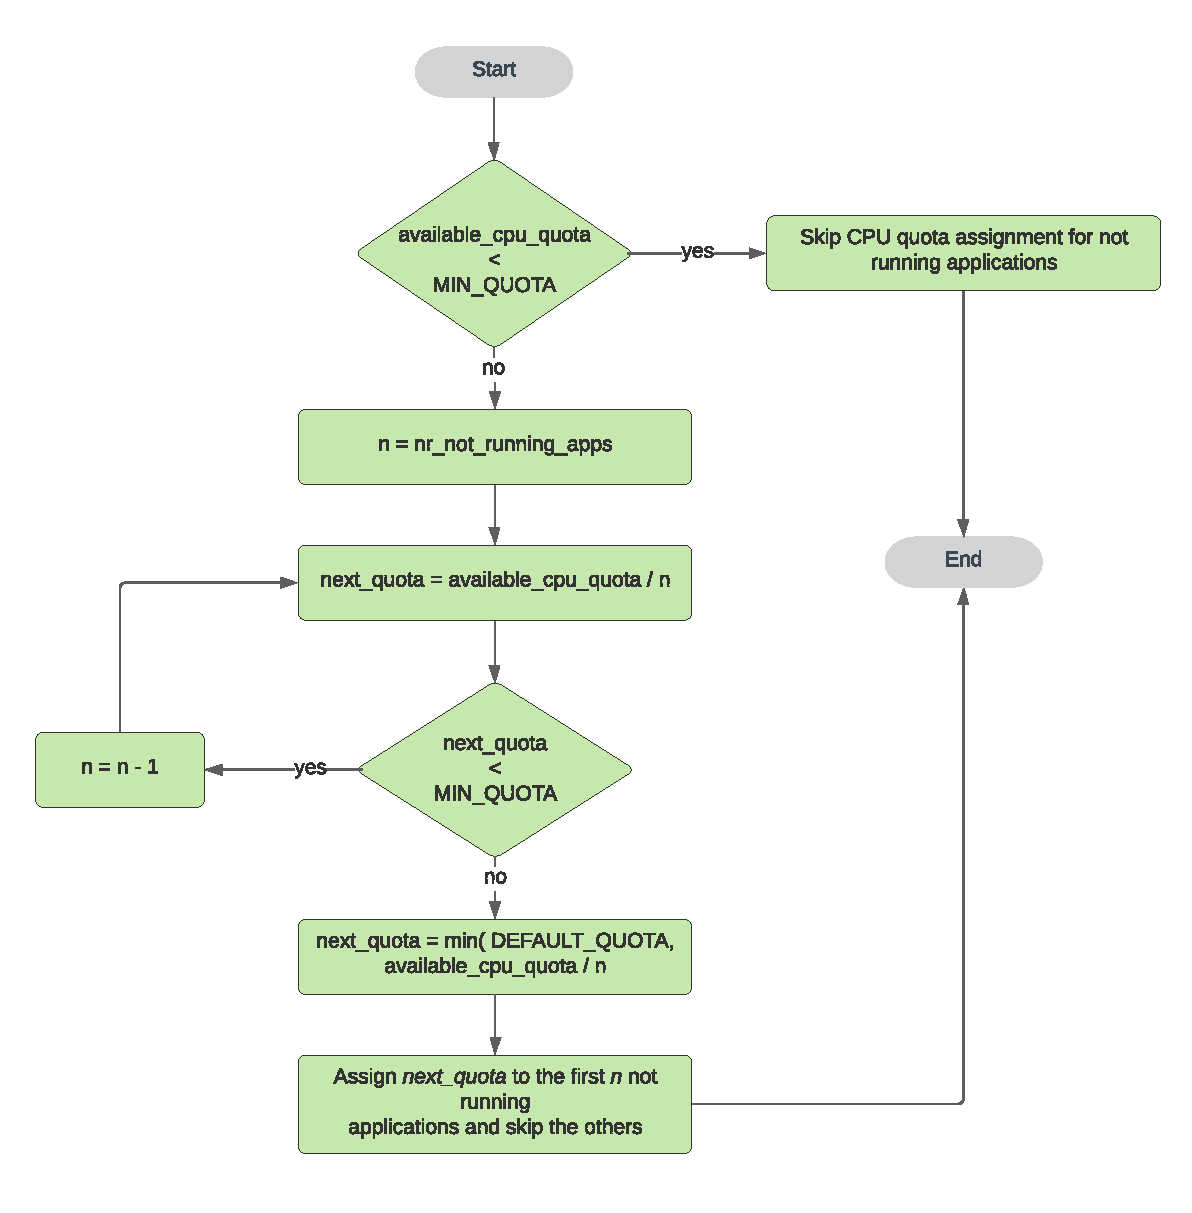
\includegraphics[width=0.9\textwidth]{not_running.pdf}
    \caption{CPU quota assignment for not running applications.}
    \label{fig:notrun}
\end{figure}
Last step of the CPU quota assignment phase of the Reliam Scheduling Policy is the computation of the quota for every application whose execution is not started yet. In this scenario we designed a \emph{fair} behaviour, i.e. a uniform CPU quota allocation among the scheduled applications. The CPU quota allocated for each application will be bounded between two constant values, \verb MIN_QUOTA \ and \verb DEFAULT_QUOTA \, depending on the \verb available_cpu_quota \ and on the number of pending applications. More specifically, it might happen that, if a fair assignment does not allow the allocation to be in the range of values mentioned above, a number of applications will not be scheduled for execution. The flowchart in Figure~\ref{fig:notrun} provides the details about how the assignment is computed for this last set of applications.
\begin{figure}[t]
    \centering
    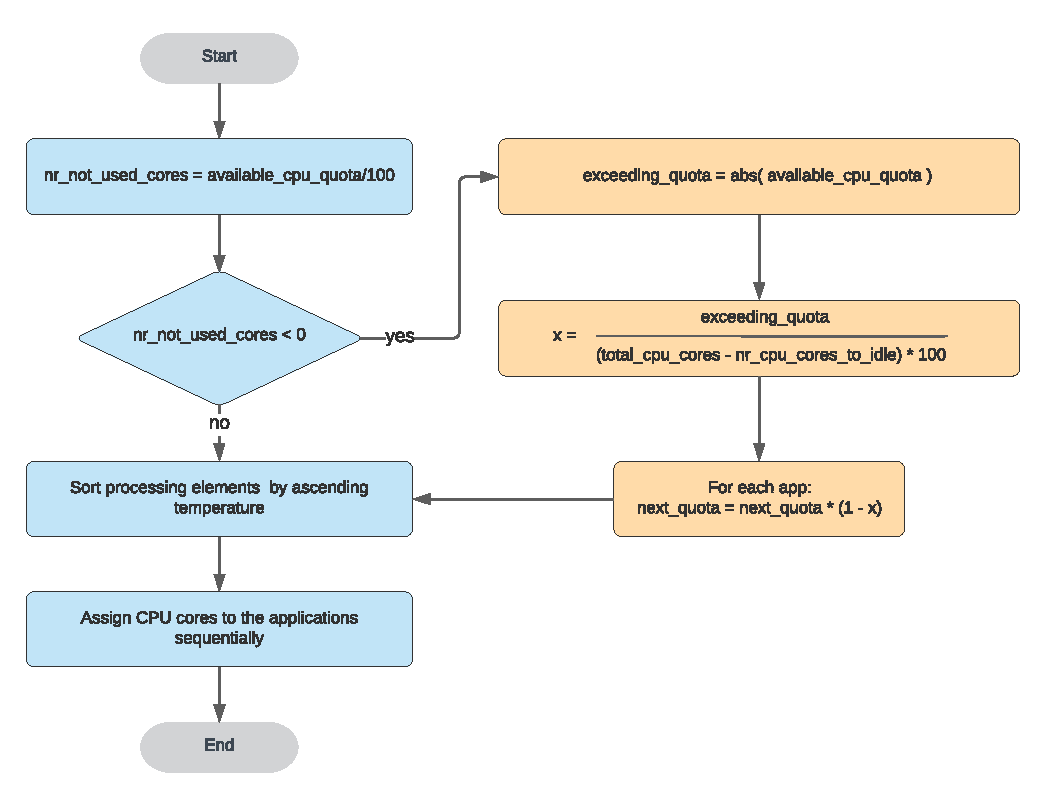
\includegraphics[width=\textwidth]{quota_red.pdf}
    \caption{Cores selection and CPU quota reduction control flow.}
    \label{fig:quotared}
\end{figure}

\subsubsection{CPU quota reduction and Core selection phases}
\label{sec:coresel}
Apart from the case of not running application, addressed by the previous paragraph, the policy allocates the CPU quota blindly with respect to the actual resources availability of the system. At each step, after being computed, the assigned CPU quota is subtracted from the variable \verb|available_cpu_quota| which, at the end of procedure, might be lower than zero. The occurrence of this event points out the fact that a CPU quota reduction is needed, since the summation of all the CPU quotas assigned by the controller is not compatible with the availability in the system, hence, it must be corrected. The CPU quota reduction has been implemented in the member function \verb|ApplyQuotaReduction()|. It computes the amount of exceeding assigned CPU quota with respect to the actually available amount as follows:
\[x = \frac{exceeding\_cpu\_quota}{(total\_nr\_cpu\_cores-nr\_cpu\_cores\_to\_idle)*100}^\text{\footnotemark}\]\cprotect\footnotetext{The denominator of this formula is the value of \verb|available_cpu_quota| at {\hyperref[sec:init]{\emph{Initialization phase}}}.}
where the numerator $exceeding\_cpu\_quota$ is computed as the absolute value of \verb|available_cpu_quota|. In the above mentioned equation, $x$ represents the ratio between the exceeding assigned CPU quota and the total allocatable amount. This ratio is used to subtract a proportional quantity of the assignment from each scheduled application, i.e. for each application, the assigned CPU quota will be reduced as follows:
\[reduced\_quota = computed\_quota * (1 - x)\]
Once, if it was needed, the CPU quota reduction phase has been completed, the selection of the cores to bind takes place. In this phase, carried out by the member function \verb|InitResourceBitset()|, a number of CPU cores is forced in idle mode by setting to zero their value in a \emph{bitset} provided by BarbequeRTRM to allow the choice of the processing elements to bind. The idled CPU cores will correspond to the ones having the highest temperature, in a number determined as:
\begin{flalign*}
nr\_idled\_cpu\_cores = max(nr\_cpu\_cores\_to\_idle,\\
nr\_cpu\_cores\_to\_idle + available\_cpu\_quota)
\end{flalign*}
where $nr\_cpu\_cores\_to\_idle$ is the value of the homonym variable defined at {\hyperref[sec:init]{\emph{Initialization phase}}}.

\subsubsection{Cores binding phase}
For each application, the binding of the CPU cores is implemented in the member function \verb|AssignWorkingMode()| and follows the the generic procedure provided by BarbequeRTRM, summarized below:
\begin{enumerate}
    \item A \verb|WorkingMode| object is instantiated;
    \item A resource requests is added, containing the generic path of the  CPU resources, the CPU quota and the way in which it must be split among the resources\cprotect\footnote{As already mentioned in the {\hyperref[sec:poldesign]{\emph{Design Section}}}, a sequential policy is used in this work.};
    \item The binding of such request to the registered resources is finalized, specifying the bitset initialized in the {\hyperref[sec:coresel]{\emph{Core selection phase}}}.
\end{enumerate}

\phantomsection
%
%\addcontentsline{toc}{chapter}{ExperimentalEvaluation}
%
\chapter{Experimental Evaluation}
%
\markboth{ExperimentalEvaluation}{ExperimentalEvaluation}	% headings
%
\label{cap:experimental}
In this section the experiments performed to test the effectiveness of the \emph{Dynamic Checkpoint Rate Tuning} and the \emph{Reliam Resource Allocation Policy} will be examined and the results will be analyzed.
\section{Experimental setup}
We performed several experiments in order to evaluate the work proposed by this thesis. in order to test the \emph{Dynamic Checkpoint Tuning} and the CPU quota allocation component of the \emph{Reliam Resource Allocation Policy} we used a high-end workstation, having a quad-core processor \emph{Intel i7-3770} on an x86\_64 architecture. The computer is provided with a 32GB \emph{RAM} and runs a \emph{Linux} operating system, with kernel version 4.15.0.

In our experiments, we used \emph{benchmarks} as workload to evaluate pros and cons of our work and provide the reader with a guideline on the use of the proposed tools with respect to the use cases.

\subsection{The NAS Parallel Benchmark Suite}
The NAS Parallel Benchmark Suite (NPB) \cite{doi:10.1177/109434209100500306} is a benchmark suite developed by the NASA Advanced Supercomputing Division, designed to evaluate the performances of parallel supercomputers. It is composed of five kernels and three pseudo-applications, available in commonly-used programming models like MPI and OpenMP and in a variety of predefined problem sizes.
The five kernels of the suite are:
\begin{itemize}
\item IS - Integer Sort
\item EP - Embarrassingly Parallel 
\item CG - Conjugate Gradient
\item MG - Multi-Grid on a sequence of meshes 
\item FT - discrete 3D fast Fourier Transform
\end{itemize}
While the three pseudo applications are:
\begin{itemize}
\item BT - Block Tri-diagonal solver
\item SP - Scalar Penta-diagonal solver
\item LU - Lower-Upper Gauss-Seidel solver
\end{itemize}

In our experimental evaluation of the \emph{Dynamic Checkpoint Rate Tuning}, we exploited the three pseudo applications. We excluded from our tests classes S, W, A and B, due to their small problem size, which causes an execution time too short to be representative for the sake of our research. Conversely, we excluded classes E and F, respectively, the former for its too long execution time and the latter for limitations in terms of memory of the hardware at our disposal. In the end, we selected both class C and D to perform an analysis aware of different workloads and a diversity of execution times. 

\subsection{The PARSEC Benchmark Suite}
The PARSEC Benchmark Suite \cite{7849432} is a benchmark suite for multiprocessor systems firstly developed by Intel and Princeton University. It is composed by thirteen applications, whose domain and type of parallelization is summarized in Table~\ref{tab:parsec}.

\begin{table}
    \centering
    \begin{tabular}{|l|l|l|}
    \hline
    \rowcolor{lightblue}\textbf{BENCHMARK} & \textbf{DOMAIN} & \textbf{PARALLELIZATION}\\
    \hline
        \rowcolor{odd}Blackscholes & Financial Analysis & Data-parallel\\
        \rowcolor{even}Bodytrack & Computer Vision & Pipeline \\
        \rowcolor{odd}Canneal & Engineering & Data-parallel  \\
        \rowcolor{even}Dedup & Enterprise Storage & Pipeline  \\
        \rowcolor{odd}Facesim & Animation & Data-parallel \\
        \rowcolor{even}Ferret & Similarity Search & Pipeline \\
        \rowcolor{odd}Fluidanimate & Animation & Data-parallel \\
        \rowcolor{even}Freqmine & Data Mining & Data-parallel \\
        \rowcolor{odd}Raytrace & Data Mining & Data-parallel \\
        \rowcolor{even}Streamcluster & Financial Analysis & Data-parallel \\
        \rowcolor{odd}Swaptions & Media Processing & Data-parallel \\
        \rowcolor{even}Vips & Media Processing & Pipeline \\
        \hline
    \end{tabular}
    \caption{Workload of PARSEC benchmarks \cite{princetonuniversity}.}
    \label{tab:parsec}
\end{table}

Each benchmark is provided with three sets of inputs, intended, respectively, for testing, simulation and execution on real machines. Benchmarks are also provided with large working sets, even with a relatively constrained input set \cite{7849432}, which grow either proportionally to the data set size or to the number of cores.

For our experimental evaluation of the mathematical model behind the quota assignment of the Reliam Resource Allocation Policy, we used the Fluidanimate PARSEC benchmark, launched with 2 threads processing 400 frames of the \emph{native} input set, i.e. the one intended for real machines. The choice of a contained number of thread allowed us to observe the behavior of the modified PID controller in all three cases of quota allocation output:  scarce, in excess and approximately correct.

\subsection{Data Center Workload and Resource Management Simulator}
\label{sec:dcworms}
The Data Center Workload and Resource Management Simulator (DCworms) is an event-driven simulation tool, written in Java, which enables modeling and simulation of computing infrastructures to estimate their performance, energy consumption and energy efficiency metrics for diverse workloads and management policies \cite{DCworms}. DCworms allows a big margin of customization with respect to workload and computational resources modeling, providing the possibility of plugging in thermal, power and reliability models. It offers a multi-level description of the incoming jobs, whose abstraction level is depicted in Figure~\ref{fig:tasks}.
\begin{figure}
    \centering
    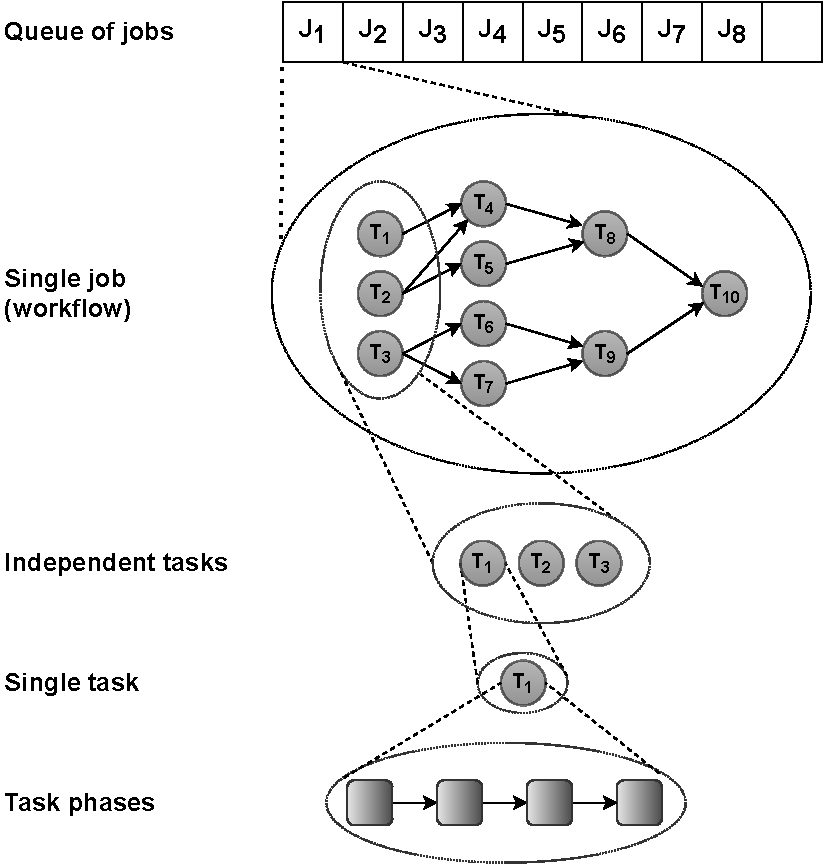
\includegraphics[width=0.8\textwidth]{dcworms_task.pdf}
    \caption{Levels of information about jobs in DCworms \cite{DCworms}.}
    \label{fig:tasks}
\end{figure}
Each task is described as a sequence of phases, periods of time in which the system is stable in terms of load, network and memory, in which the impact on the resources is observable. A simulated value representing the resource consumption profile is linked to each phase. 

In this thesis, we used DCworms to simulate the effect of the reliability-aware decisions performed by the \emph{Reliam Resource Allocation Policy} on a multi-node scale. We plugged a reliability model in the simulator linearly dependent on the temperature, which, in turn, has been modeled as dependent on the CPU load.

More specifically, the temperature profile is modeled as described by Leva et al. in \cite{leva2018}:
\begin{enumerate}
    \item The thermal state is updated:
    \begin{flalign*}
    &state = (0.03 * state + 22 * timeStep * cpuLoad) / (timeStep+ 0.03)&
\end{flalign*}
    \item The current temperature is computed:
    \begin{flalign*}
        & temp = state + 30&
    \end{flalign*}
\end{enumerate}

Given the function \verb|GetTemperature()|, implementing the thermal model, the reliability value is computed as described in Algorithm~\ref{alg:rel_model}.

\begin{algorithm}
    \SetKwInput{KwInput}{Input}
    \SetKwInput{KwConstant}{Constant}% Set the Input
    \SetKwInput{KwOutput}{Output}              % set the Output
    \DontPrintSemicolon
    \BlankLine

    \KwInput{CPU load \emph{cpuLoad}}
    \KwInput{Last observed thermal state \emph{state}}
    \KwInput{Random number \emph{rand}}
    \KwConstant{Stress temperature \emph{tStress}}
    \KwOutput{Reliability level \emph{rel}}
    %\BlankLine
    \algrule
    

\BlankLine
\SetKwFunction{Funcs}{GetReliability}
\SetKwProg{Fn}{double}{:}{}
\Fn{\Funcs{\KwSty{int} cpuLoad, \KwSty{float} rand, \KwSty{float} state}}{

\KwSty{float} temp = GetTemperature(cpuLoad, state)\;
    \KwSty{double} rel = (1-temp/tStress)*(1-rand)\;
    \KwRet rel\;
 }
    \BlankLine
   \caption{Reliability model implementation.}
   \label{alg:rel_model}
\end{algorithm}


We set $100^\circ$C as stress temperature, while using the \emph{rand} term to model the increase of the slope in the reliability curve after a certain threshold. More specifically, we defined the \emph{criticality threshold} as the percentage X such that:
\begin{align*}
    \begin{cases}
        0<rand<1 & \qquad \text{if }\frac{temp}{tStress}*100 \geq X\\
        \noalign{\vskip6pt}
        rand = 0 &\qquad \text{otherwise}
    \end{cases}
\end{align*}

\section{Dynamic Checkpoint Rate Tuning}
As deeply examined in {\hyperref[sec:dcrt]{Section~\ref{sec:dcrt}}}, aim of the Dynamic Checkpoint Rate Tuning is to tune an application specific interval between two consecutive checkpoints in order to meet time requirements and/or reliability goals. In order to test the effectiveness of our solution in different scenarios, we designed our model as explained in the following.

Given an application, we define its total time $T_{TOT}$ as: 
\begin{align}\label{eq:1}
    T_{TOT} = T_{exc\_tot} + T_{chk\_tot}
\end{align}

where \(T_{exc\_tot}\) and \(T_{chk\_tot}\) are, respectively, the time passed executing the code of the application and the time passed performing checkpoints. Considering the existence of a constant hazard function $h(z) = \lambda$, defined as the rate of occurrence of a failure in an hour, and given $R(t)$, a function that outputs the time passed between the last available checkpoint and the restart of the application, we can formulate $T_{failure}$, the additional time spent in case of failure, and build the following system of equations:  
\begin{align}\label{eq:2}
    \begin{cases}
    T_{TOT} = T_{exc\_tot} + T_{chk\_tot}\\
    \noalign{\vskip9pt}
    T_{failure} =  \displaystyle\int_0^{T_{TOT}}\lambda * R(t)dt
    \end{cases}
\end{align}
$R(t)$ is, in turn, composed by $T_{rst}$, the time spent restarting the application, and $T_{re\_exc}$, the time passed re-executing the piece of code whose execution was performed after the completion of the last checkpoint. Thus, we arrived at the following definition of $R(t)$:
\begin{align}\label{eq:3}
    R(t) = T_{rst}(t) + T_{re\_exc}
\end{align}
Since $T_{rst}$ mostly depends on human interaction and, in any case, does not depend on the logic of this component, we consider it negligible for the sake of this study, hence, from now on, we will simplify the computation of $R(t)$ as:
\begin{align}
    R(t) = T_{re\_exc}(t)
\end{align}

\begin{figure}[H]
    \centering
    \subfloat[\centering Benchmarks problem size class C.]{{\includegraphics[width=0.6\textwidth]{chk_mean_c.pdf} }}\\
    \vspace{1.1em}
    \subfloat[\centering Benchmarks problem size class D.]{{\includegraphics[width=0.6\textwidth]{chk_mean_d.pdf} }}
    \caption{Checkpoint mean time in seconds and standard deviation of the benchmarks used in the experimental evaluation.}
    \label{fig:chk_mean}%
\end{figure}
Running the benchmarks used for this experimental evaluation, we made sure that, for each of such applications, we could approximate the duration of a checkpoint routine with the arithmetic mean of all checkpoints. In Figure~\ref{fig:chk_mean} the checkpoint mean of each used benchmark is shown, displaying that standard deviation never exceeds the 10\% of the mean. This result has two turn ups: not only we can re-write, without any loss of information, $T_{chk\_tot}$ as $n* T_{chk\_mean}$, where $n$ is the total number of performed checkpoints, but also, for construction of the \emph{Dynamic Checkpoint Rate Tuning}, we can do the same approximation also for the period between two consecutive checkpoints, hence, we can write:
\begin{align}
    T_{exc\_tot} = n*(T_{period} - T_{chk\_mean}) + T_{end}
\end{align}  
where $T_{period}$ is the arithmetic mean of the time passed between the start of two consecutive checkpoints, while $T_{end}$ is the execution time between the last checkpoint and the end of the program.
Up to this point, we re-write the system of equations \ref{eq:2} as:
\begin{align}\label{eq:4}
    \begin{cases}
    T_{TOT} = n*(T_{period} - T_{chk\_mean}) + n*T_{chk\_mean} + T_{end}\\
    \noalign{\vskip9pt}
    T_{failure} =  \displaystyle\int_0^{T_{TOT}}\lambda * R(t)dt
    \end{cases}
\end{align}
 Without any loss of information, we can neglect the term $T_{end}$ from the equation, since its value is certainly less than a checkpoint period. Simplifying,
\begin{align}
    \begin{cases}
        T_{TOT} = n*T_{period}\\
        \noalign{\vskip9pt}
        T_{failure} = \displaystyle\int_0^{T_{TOT}}\lambda * R(t)dt
    \end{cases}
\end{align}
As mentioned above, we consider the time span between the start of two consecutive checkpoints approximable with the arithmetic mean given by $T_{period}$. Thanks to this approximation, it is possible to discretize the integral of $T_{failure}$ in a summation of integrals. Those integrals will be defined between $t_{start\_exc_i}$ and $t_{end\_exc_i}$, respectively the starting time and the ending time of the execution of the application code in period $i$. Since we approximated each period with $T_{period}$ and each checkpoint time with $T_{chk\_mean}$, we find that:
\begin{align}
    t_{end\_exc_i} - t_{start\_exc_i} = T_{period} - T_{chk\_mean} = T_{exc\_mean}\qquad \forall i 
\end{align}

Starting from the assumptions just made, the computation of $T_{failure}$ becomes:

\begin{align} 
T_{failure} & = \displaystyle\int_0^{T_{TOT}}\lambda\, R(t)dt \\
 \noalign{\vskip9pt}
 & = \sum_{i=1}^n \displaystyle\int_{t_{end\_exc_i}}^{t_{start\_exc_i}}\lambda \,t_idt_i\\
  \noalign{\vskip9pt}
 & = \sum_{i=1}^n\lambda\,\frac{t_i^2}{2}\,\Bigr|_{t_{start\_exc_i}}^{t_{end\_exc_i}}\\
  \noalign{\vskip9pt}
 & = n\, \lambda\,\frac{{T_{exc\_mean}}^2}{2}\label{eq:tfailure}
\end{align}
We performed our experiments on classes C and D of the three pseudo-applications of the NPB suite, BT, LU and SP. We set $k=0.02$ for class C and $k=0.2$ for class D problem size, where $k$ is the upper bound on the overhead set by the user for the application at issue, and we plotted $T_{failure}$ as defined in Equation~\ref{eq:tfailure}, varying $\lambda$. Then, we summed the obtained $T_{failure}$ to the total overhead produced by the checkpointing routine and we plotted this sum, as well, varying $\lambda$. Results of such measurements are shown in Figures~\multiref{fig:real_c}{fig:real_d}. Finally, in Figure~\ref{fig:real_perc}, the percentage overhead caused by the sum of checkpointing time and the time to recover from a failure, on the execution of the only application code is displayed, again, varying $\lambda$.

{\captionsetup[subfloat]{labelformat=empty}
\begin{figure}
    \centering
    {
    \subcaption[]{Benchmark: BT}
    \subfloat[\centering]{{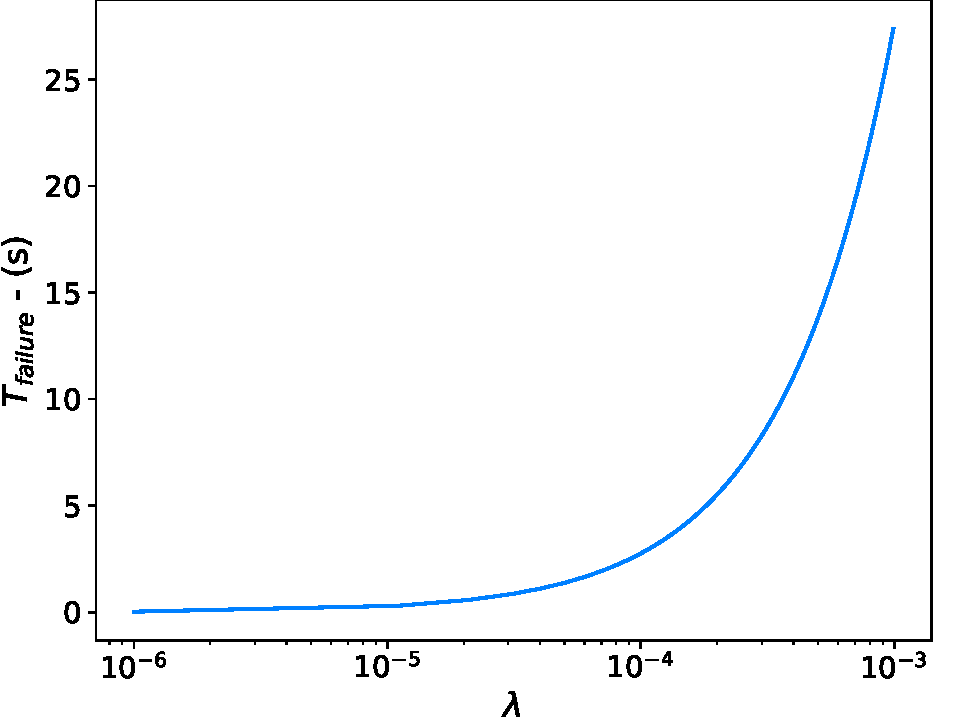
\includegraphics[width=0.49\textwidth]{avg_real_reset_time_BT_C.pdf} }}
    \subfloat[\centering]{{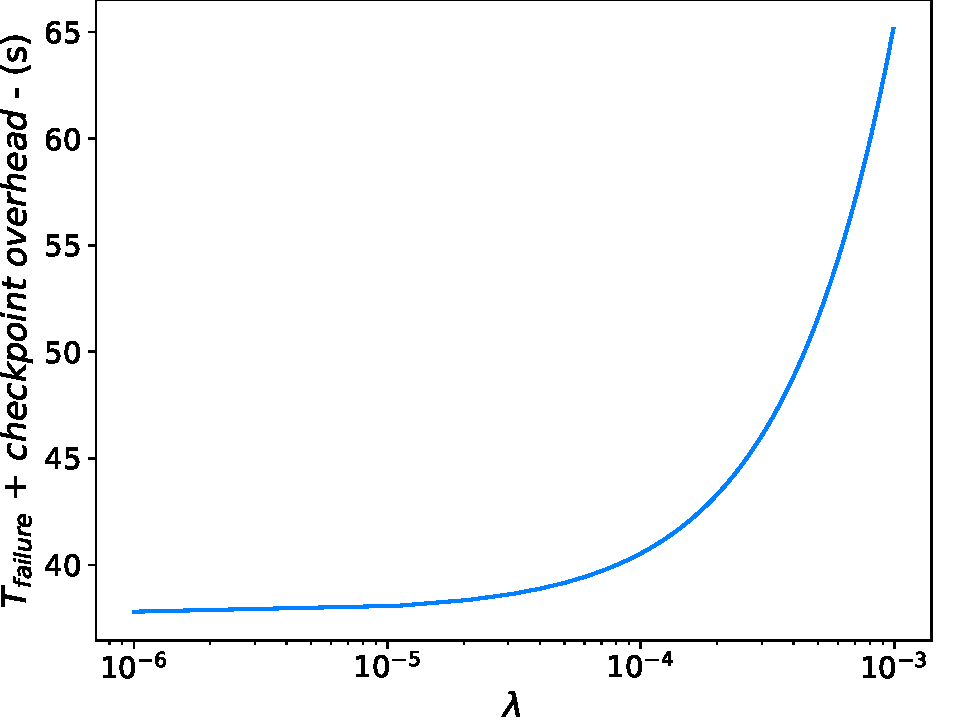
\includegraphics[width=0.49\textwidth]{avg_real_tot_ovhd_BT_C.pdf} }}\vspace{-1.1em}}
    {
    \subcaption[]{Benchmark: LU}
    \subfloat[\centering]{{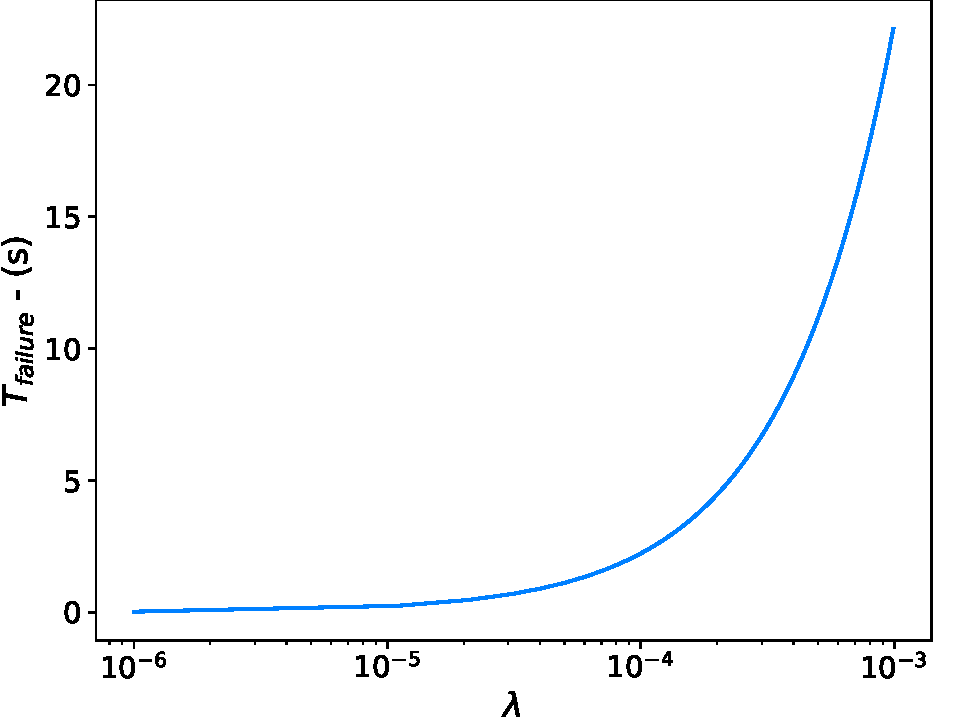
\includegraphics[width=0.49\textwidth]{avg_real_reset_time_LU_C.pdf} }}
    \subfloat[\centering]{{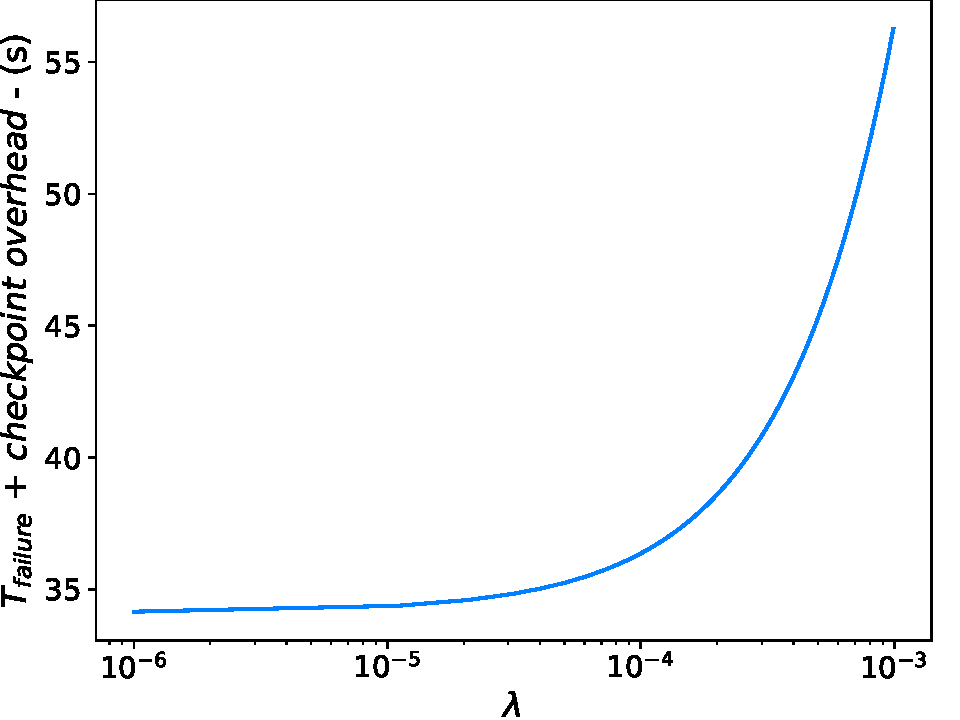
\includegraphics[width=0.49\textwidth]{avg_real_tot_ovhd_LU_C.pdf} }}\vspace{-1.1em}}
    {
    \subcaption[]{Benchmark: SP}
    \subfloat[\centering \textbf{(a)} Estimated mean overhead caused by the re-execution of application code in case of failure, varying $\lambda$.]{{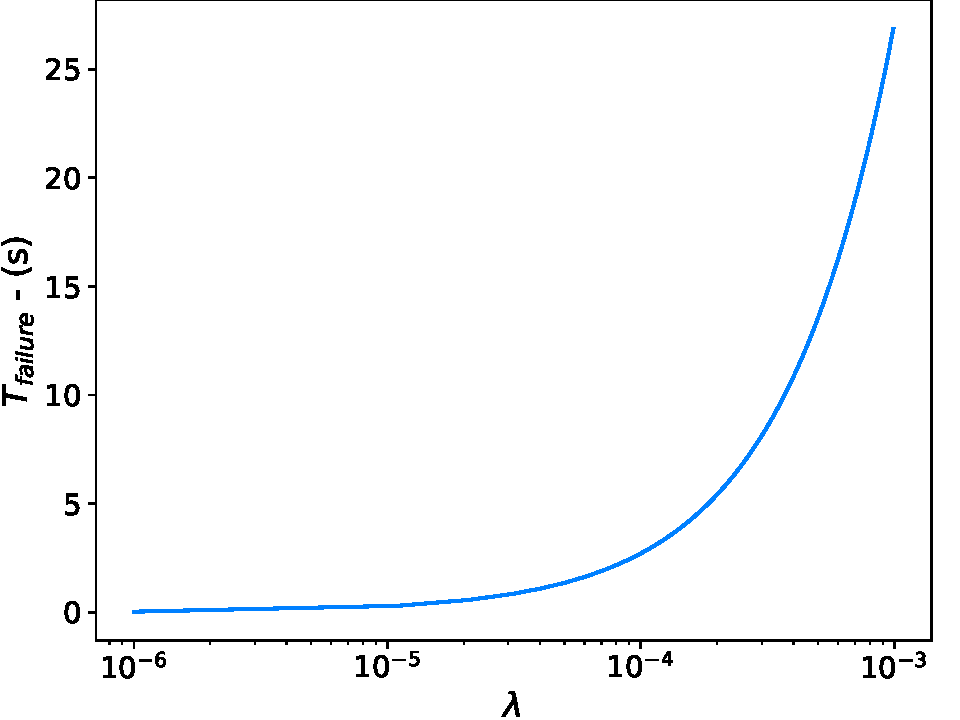
\includegraphics[width=0.49\textwidth]{avg_real_reset_time_SP_C.pdf} }}
    \subfloat[\centering \textbf{(b)} Sum of the value of \textbf{(a)} plus the checkpoint overhead, varying $\lambda$.]{{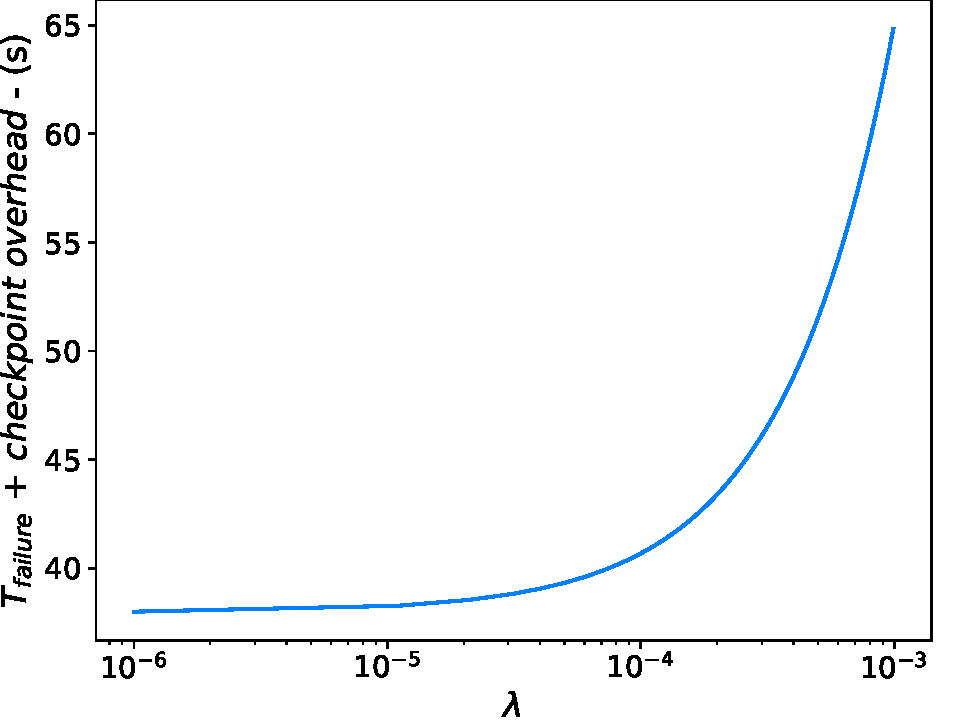
\includegraphics[width=0.49\textwidth]{avg_real_tot_ovhd_SP_C.pdf} }}}
    \caption{Plot of \textbf{(a)} $T_{failure}$, \textbf{(b)} $T_{failure}+checkpoint\ overhead$, varying $\lambda$ - Problem size class C, k=0.02, measurement in seconds.}%
    \label{fig:real_c}%
\end{figure}}

{\captionsetup[subfloat]{labelformat=empty}
\begin{figure}
    \centering
    {
    \subcaption[]{Benchmark: BT}
    \subfloat[\centering]{{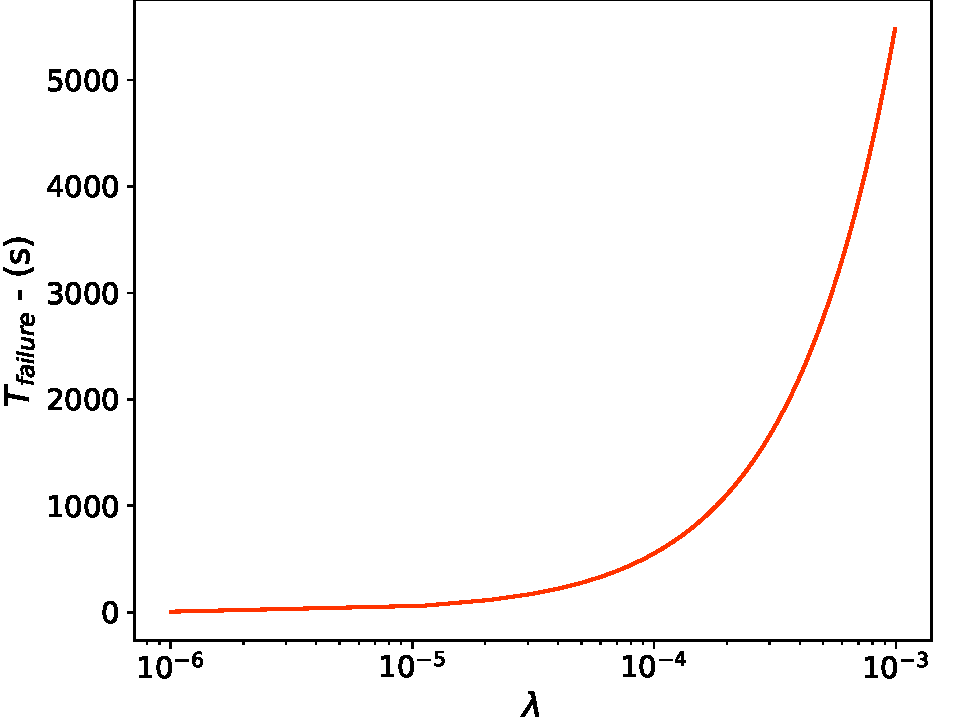
\includegraphics[width=0.49\textwidth]{avg_real_reset_time_BT_D.pdf} }}
    \subfloat[\centering]{{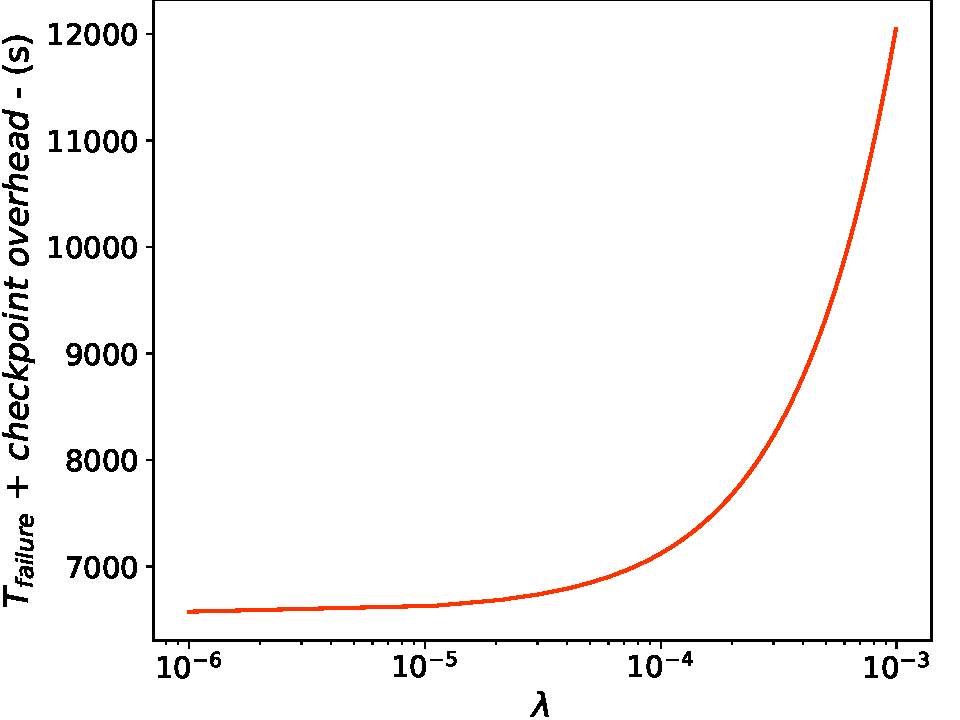
\includegraphics[width=0.49\textwidth]{avg_real_tot_ovhd_BT_D.pdf} }}\vspace{-1.1em}}
    {
    \subcaption[]{Benchmark: LU}
    \subfloat[\centering]{{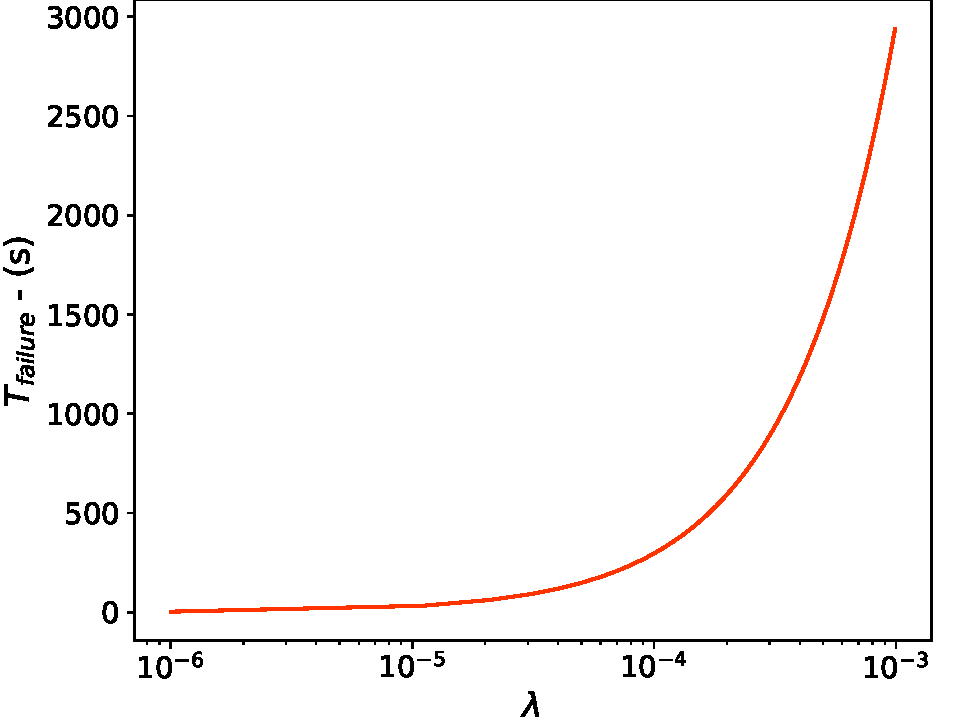
\includegraphics[width=0.49\textwidth]{avg_real_reset_time_LU_D.pdf} }}
    \subfloat[\centering]{{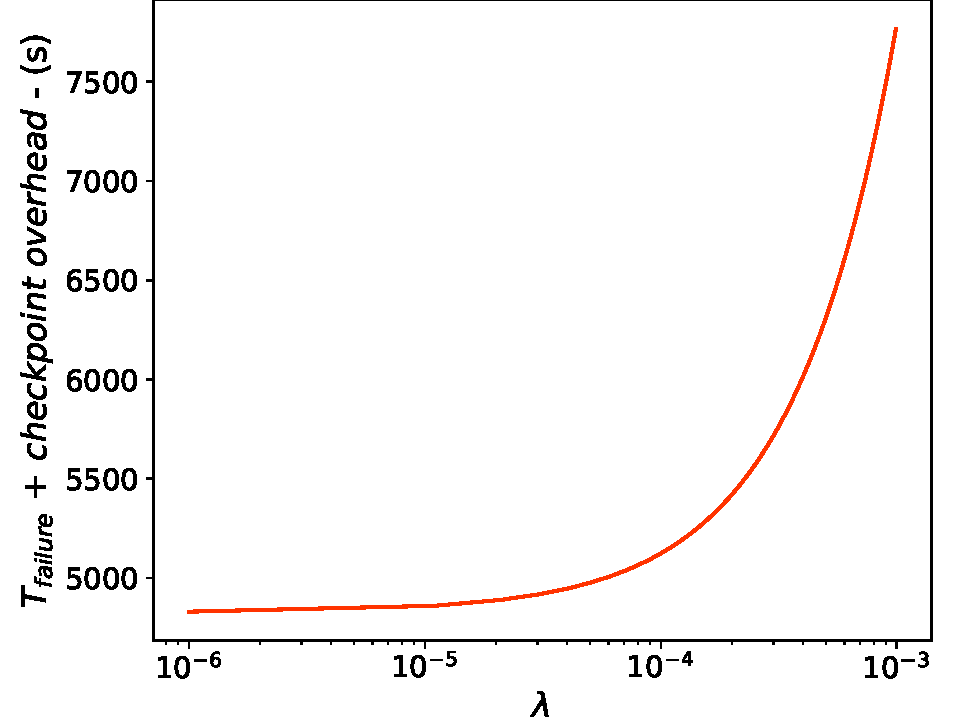
\includegraphics[width=0.49\textwidth]{avg_real_tot_ovhd_LU_D.pdf} }}\vspace{-1.1em}}
    {
    \subcaption[]{Benchmark: SP}
    \subfloat[\centering \textbf{(a)} Estimated mean overhead caused by the re-execution of application code in case of failure, varying $\lambda$.]{{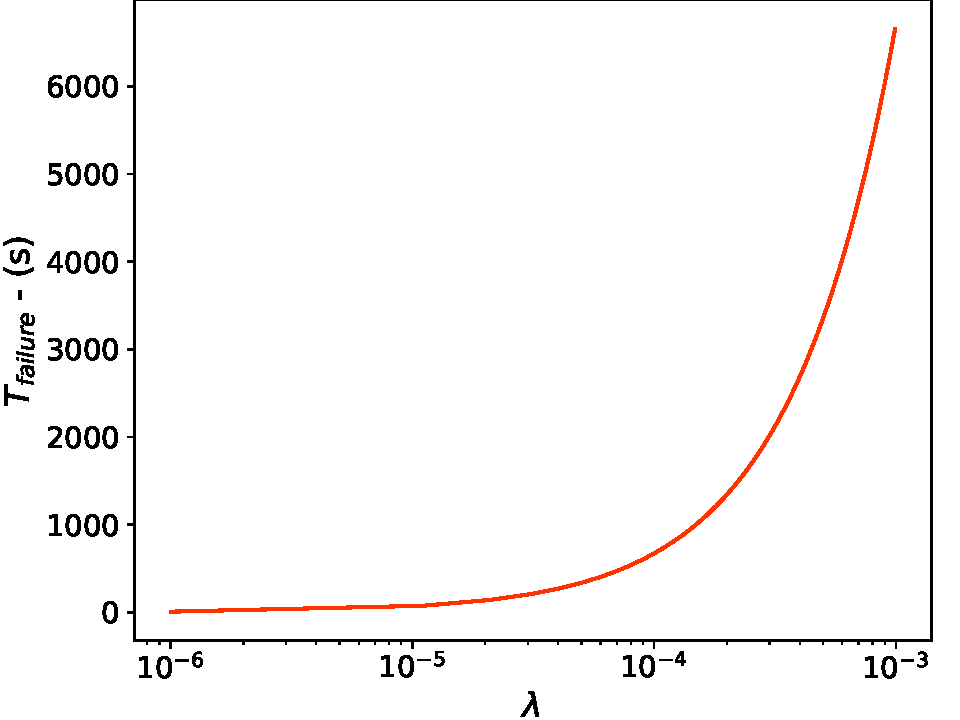
\includegraphics[width=0.49\textwidth]{avg_real_reset_time_SP_D.pdf} }}
    \subfloat[\centering \textbf{(b)} Sum of the value of \textbf{(a)} plus the checkpoint overhead, varying $\lambda$.]{{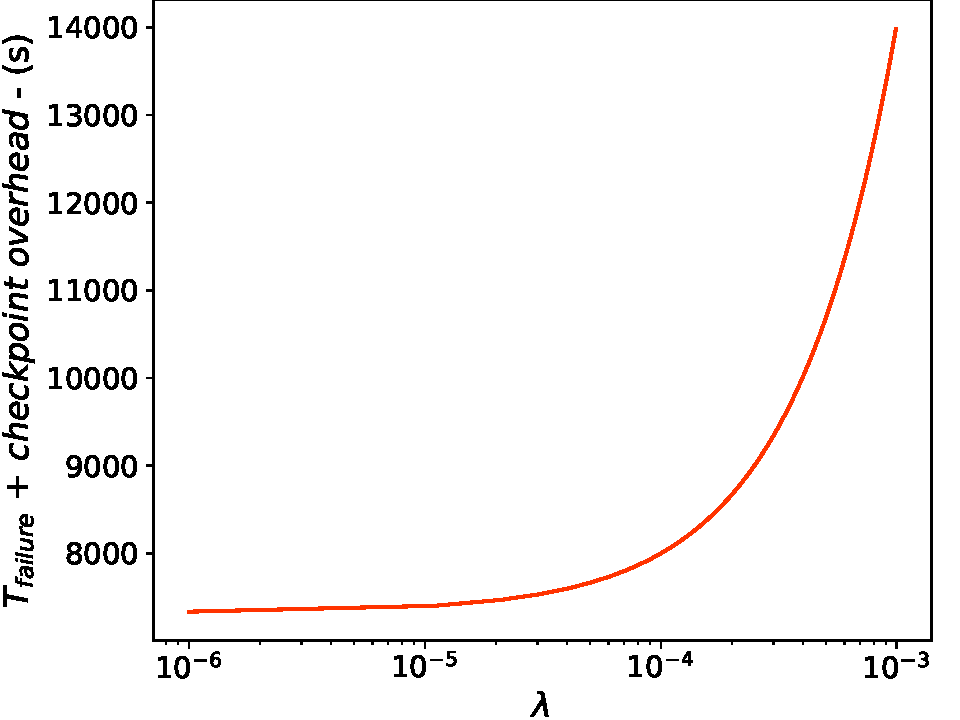
\includegraphics[width=0.49\textwidth]{avg_real_tot_ovhd_SP_D.pdf} }}}
    \caption{Plot of \textbf{(a)} $T_{failure}$, \textbf{(b)} $T_{failure}+checkpoint\ overhead$, varying $\lambda$ - Problem size class D, k=0.2, measurement in seconds.}%
    \label{fig:real_d}%
\end{figure}}

{\captionsetup[subfloat]{labelformat=empty}
\begin{figure}
    \centering
    {
    \subcaption[]{Benchmark: BT}
    \subfloat[\centering]{{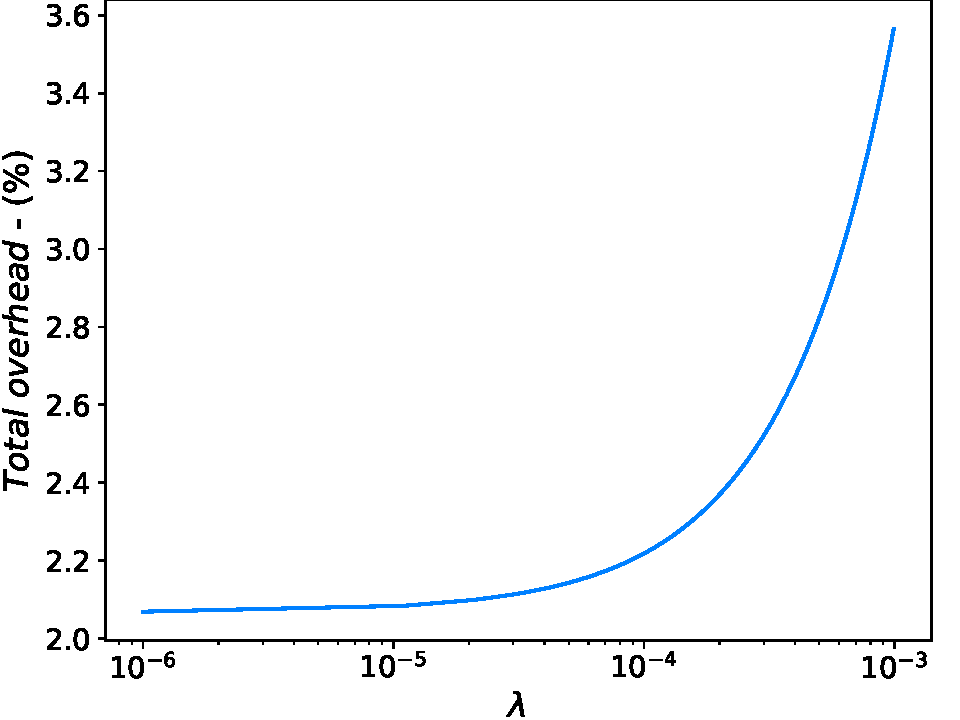
\includegraphics[width=0.49\textwidth]{real_perc_tot_ovhd_BT_C.pdf} }}
    \subfloat[\centering]{{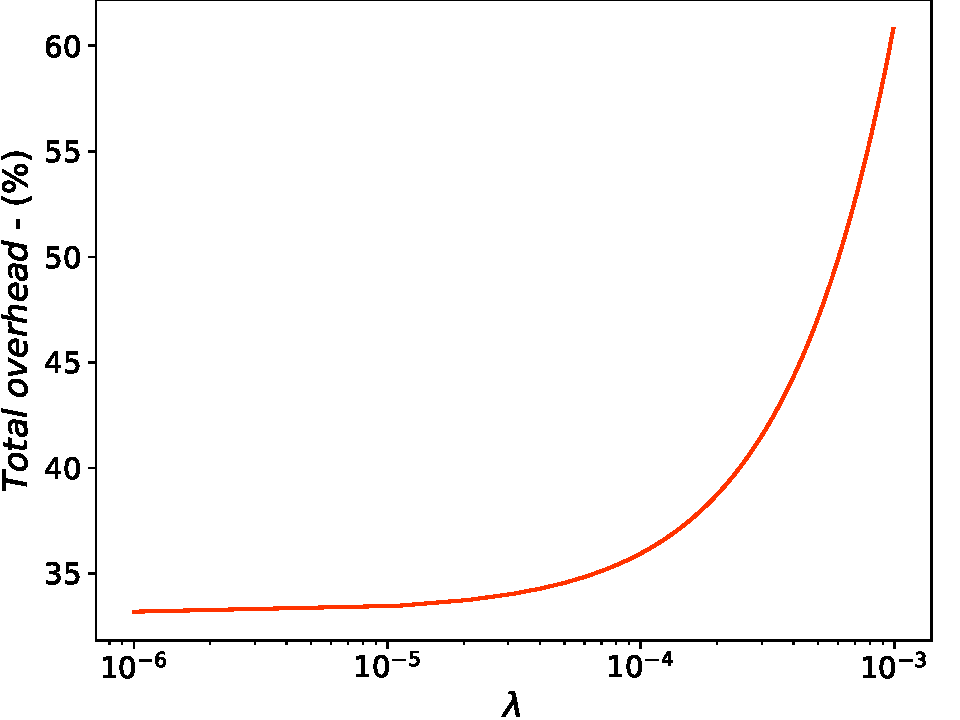
\includegraphics[width=0.49\textwidth]{real_perc_tot_ovhd_BT_D.pdf} }}\vspace{-1.1em}}
    {
    \subcaption[]{Benchmark: LU}
    \subfloat[\centering]{{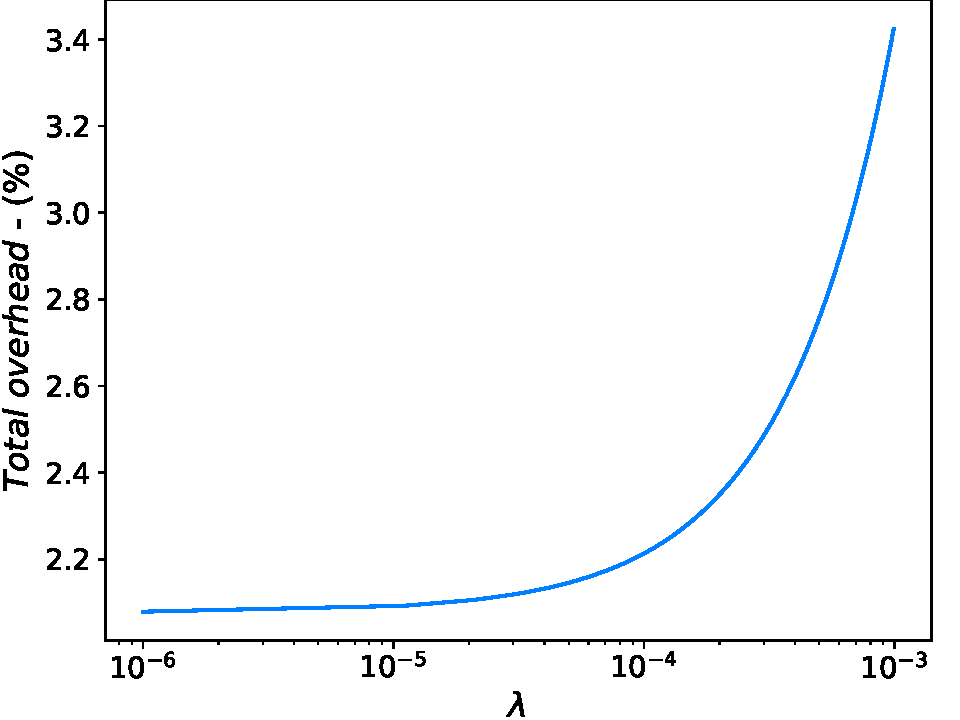
\includegraphics[width=0.49\textwidth]{real_perc_tot_ovhd_LU_C.pdf} }}
    \subfloat[\centering]{{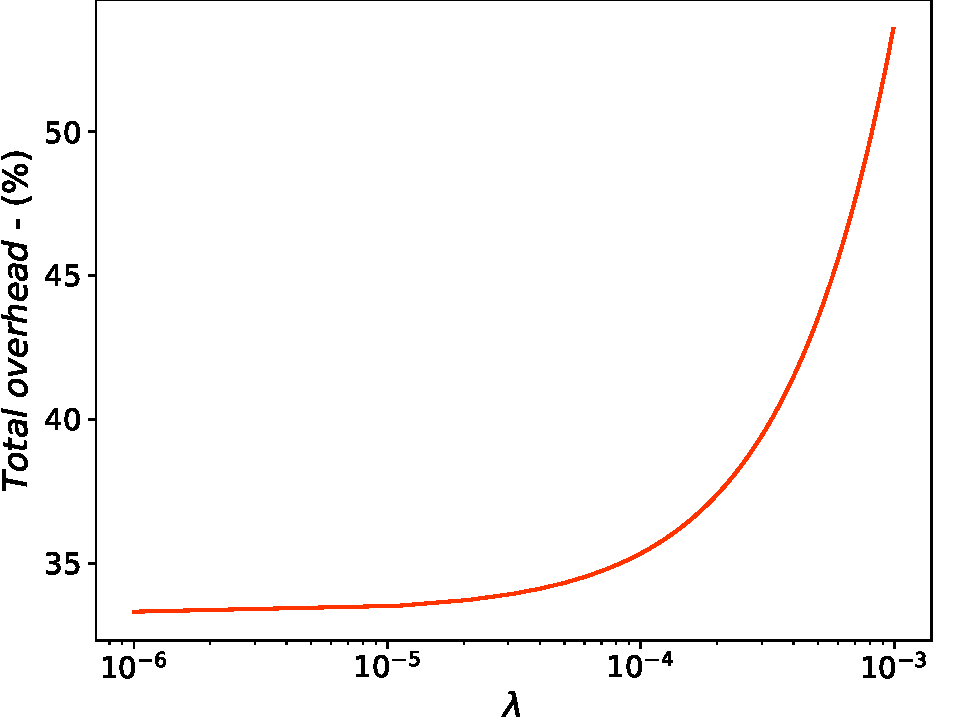
\includegraphics[width=0.49\textwidth]{real_perc_tot_ovhd_LU_D.pdf} }}\vspace{-1.1em}}
    {
    \subcaption[]{Benchmark: SP}
    \subfloat[\centering \textbf{(a)} Problem size class C - $k=0.02$.]{{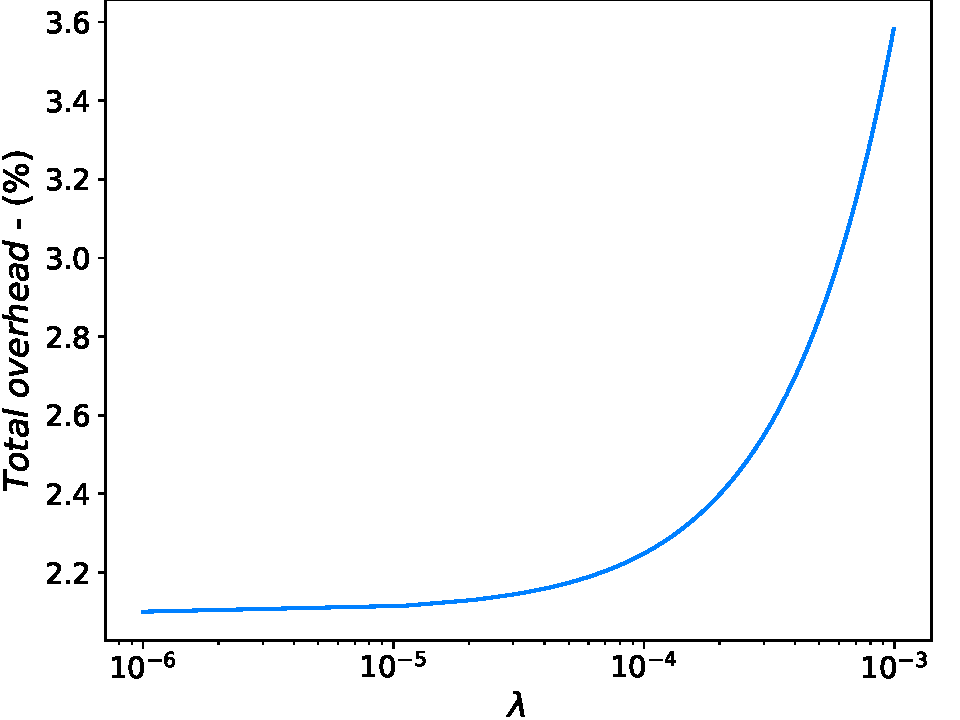
\includegraphics[width=0.49\textwidth]{real_perc_tot_ovhd_SP_C.pdf} }}
    \subfloat[\centering \textbf{(b)} Problem size class D - $k=0.2$.]{{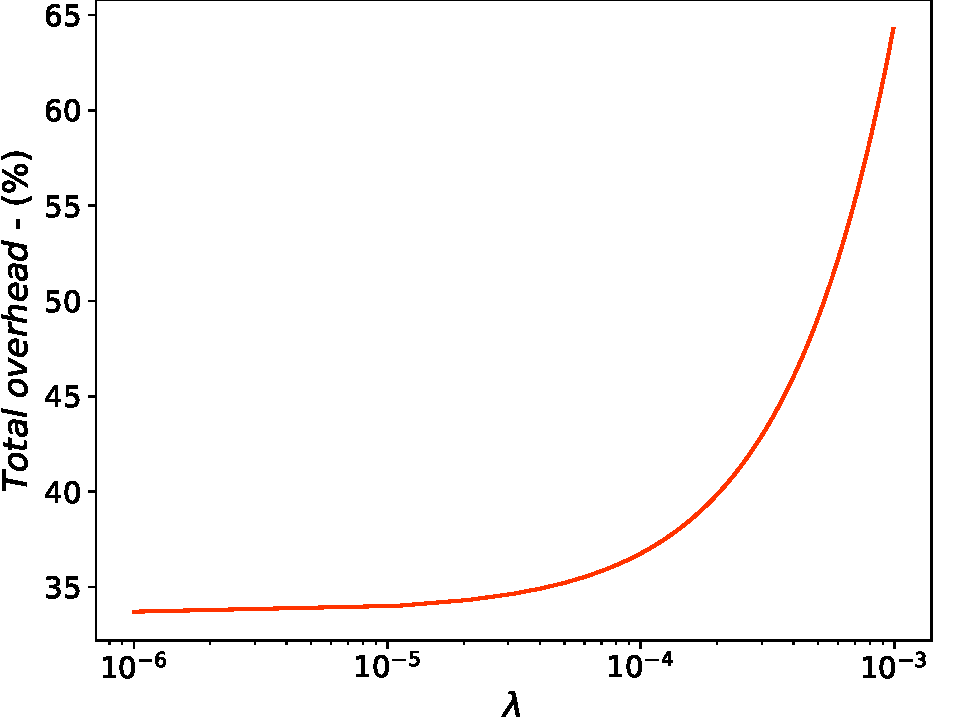
\includegraphics[width=0.49\textwidth]{real_perc_tot_ovhd_SP_D.pdf} }}}
    \caption{Percentage overhead caused by the sum of checkpointing time and time to recover from a failure, varying $\lambda$, on the execution of the sole application code.}%
    \label{fig:real_perc}%
\end{figure}}

From the above mentioned plots, it is possible to notice that, as expected, although it is possible to bound the overhead caused by the performing of the checkpoints, in the case of a reliability critical system, the overhead caused by failures might highly endanger the performance of the execution anyways. More specifically, Figure~\ref{fig:real_perc}(a) shows how, on one hand, for smaller problem sizes, hence shorter execution and checkpoint times, the percentage overhead, including the time to recover from a failure, does not exceeds \emph{significantly} in absolute value the upper bound set for the application. In this case, an overhead of 2\% was tolerated, and, in a highly unreliable system, a maximum of cumulative 3.6\% overhead is registered. On the other hand, for bigger problem sizes, Figure~\ref{fig:real_perc}(b), setting an upper bound of 20\% on the overhead, while the trend is about the same, a higher failure rate significantly impacts on the performance, getting close to the the 65\% of the application code execution time, in the case of SP benchmark. The choice of a higher upper bound in the case of bigger problem sizes has been determined by a matter of common sense: with a value as small as the one provided for class C problem sizes, given the extended $T_{chk\_mean}$ and $T_{exc\_tot}$ of class D, the number of checkpoints completed at the end of the execution of the application would have been too few for a realistic HPC use case.

To generalize these results, we carried out some computation on our measurement, in order to evaluate the just mentioned results for a wider range of reasonable values of $k$. Exploiting the fact that real checkpoint and period times can be easily approximated by their mean, we estimated the results commented above, using different values of $k$. 

For construction of the \emph{Dynamic Checkpoint Rate Tuning}, we know that:
\begin{align}
    n*T_{chk\_mean} &= k*n*(T_{period} - T_{chk\_mean})\label{eq:extract}\\
    T_{chk\_mean} &= k*(T_{period} - T_{chk\_mean})\\
    (k+1)*T_{chk\_mean} &= k*T_{period}\\
    T_{period} &= \frac{(k+1)}{k}*T_{chk\_mean}\label{eq:period}
\end{align}

Moreover, in light of the result obtained in Equation~\ref{eq:period} and reminding that:
\begin{align}
    T_{exc\_tot} = n*(T_{period} - T_{chk\_mean})
\end{align}
where $T_{exc\_tot}$ is known, we can also extract $n$ as follows:
\begin{align}
    T_{exc\_tot} &= n*\left(\frac{(k+1)}{k}*T_{chk\_mean} - T_{chk\_mean}\right)\\
    \noalign{\vskip9pt}
    T_{exc\_tot} &= n * \frac{T_{chk\_mean}}{k}\\
    \noalign{\vskip9pt}
    n &= k * \frac{T_{exc\_tot}}{T_{chk\_mean}}
\end{align}

Figures~\multiref{fig:comp_c}{fig:comp_perc} show the same measurements of Figures~\multiref{fig:real_c}{fig:real_perc} for a wide range of reasonable values of $k$.

Confirming the expectations given by the previous plots, we can observe that, although lower values of $k$ lead to higher values of $T_{failure}$, they are nonetheless suggested for smaller sized applications, since diminishing the overhead caused by the time spent re-executing lost computation, does not entails a smaller overhead, not even in a reliability critical system, such as the one characterized by $\lambda=10^{-3}$. Conversely, a bigger problem size, combined to a higher failure rate, might lead to an inversion of this trend. Figures~\ref{fig:comp_d}(b)~and~\ref{fig:comp_perc}(b) show how, with lower values of $k$, not only the total overhead significantly grows with the growing of $T_{failure}$, but also, for values of $\lambda$ \emph{high enough}, it might exceed the total overhead produced by a bigger $k$. More specifically, it is possible to see how, with $k=0.05$ (i.e. upper bound of 5\% in the checkpoint time overhead), while, in reliability safe systems, we measure a reasonably low overhead, around values of $\lambda=10^{-4}$, for all of the three benchmarks, it not only doubles its impact, but also exceeds the one produced by higher values of $k$. The conclusion of this evaluation is that, although, in reliable systems, the choice of the $k$ parameter is directly proportional to the amount of total overhead caused by both checkpoint time and time to recover from a failure, in systems where failures occurs with a higher frequency, the problem size is to consider in order not to lose the gain in specificity provided by the \emph{Dynamic Checkpoint Rate Tuning}. For this reason, a framework like BarbequeRTRM, in which the system state is constantly monitored and the checkpoint rate is tuned and adapted to each specific application, is an important resource for a better exploitation of HPC potentialities.

{\captionsetup[subfloat]{labelformat=empty}
\begin{figure}
    \centering
    {
    \subcaption[]{Benchmark: BT}
    \subfloat[\centering]{{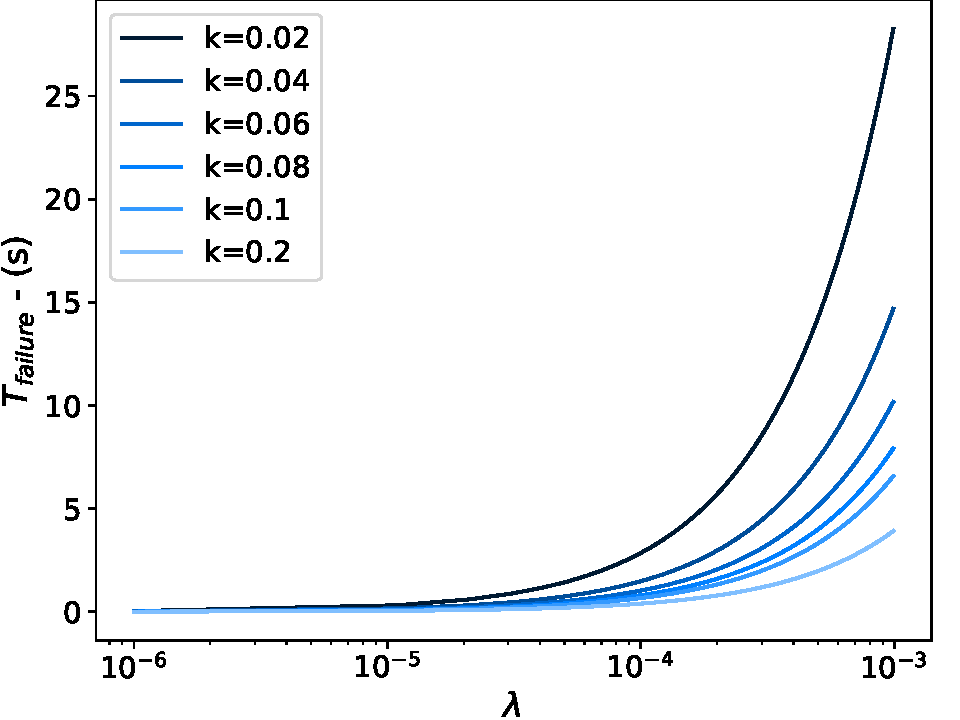
\includegraphics[width=0.49\textwidth]{avg_reset_time_BT_C.pdf} }}
    \subfloat[\centering]{{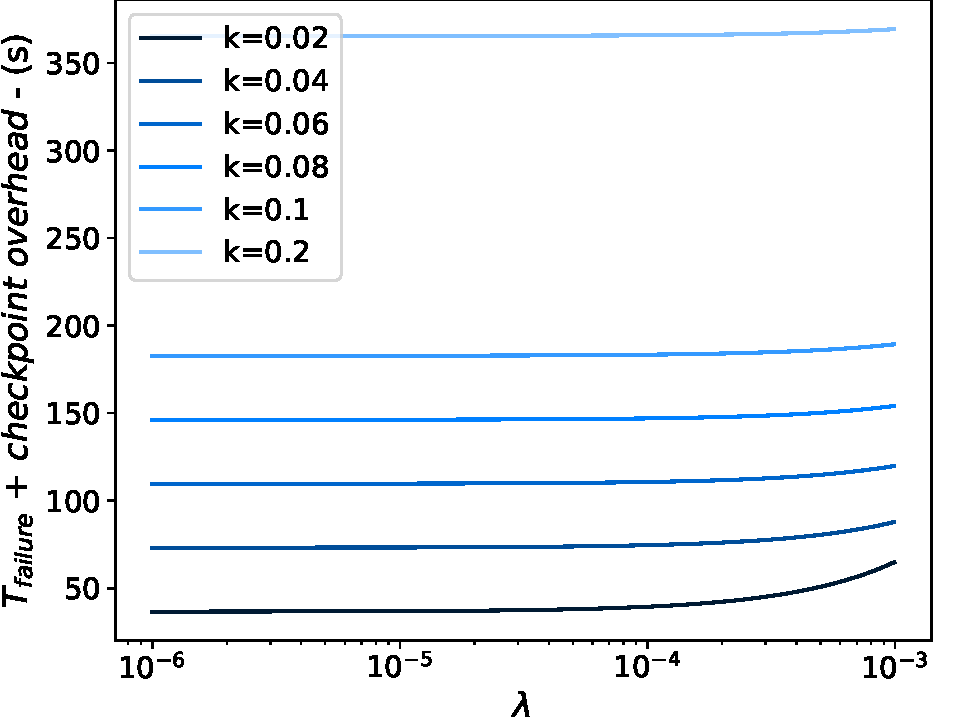
\includegraphics[width=0.49\textwidth]{avg_tot_ovhd_BT_C.pdf} }}\vspace{-1.1em}}
    {
    \subcaption[]{Benchmark: LU}
    \subfloat[\centering]{{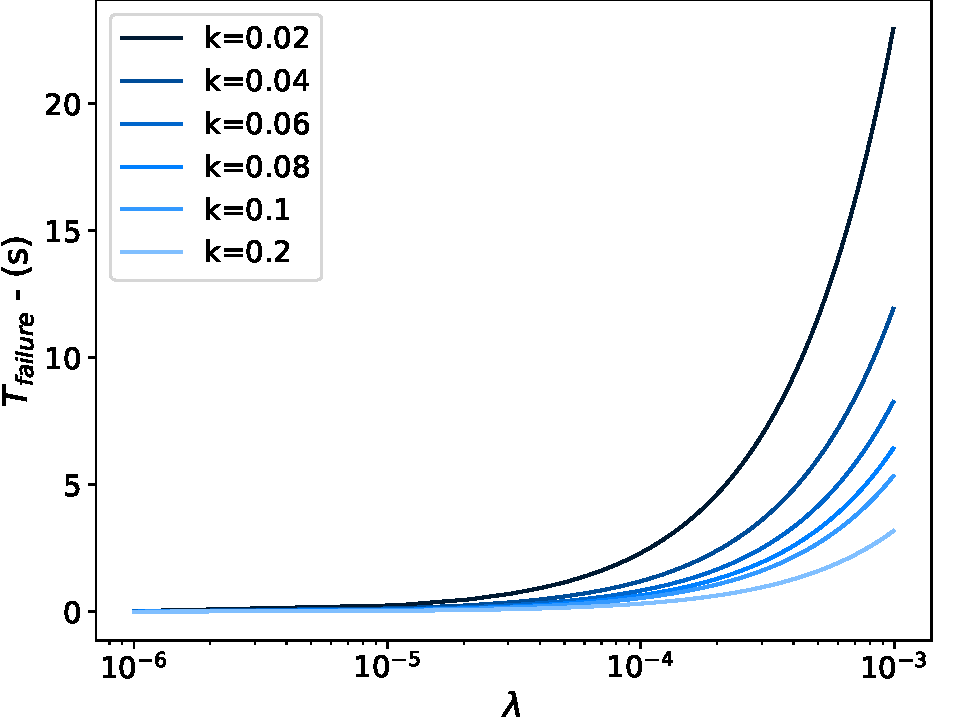
\includegraphics[width=0.49\textwidth]{avg_reset_time_LU_C.pdf} }}
    \subfloat[\centering]{{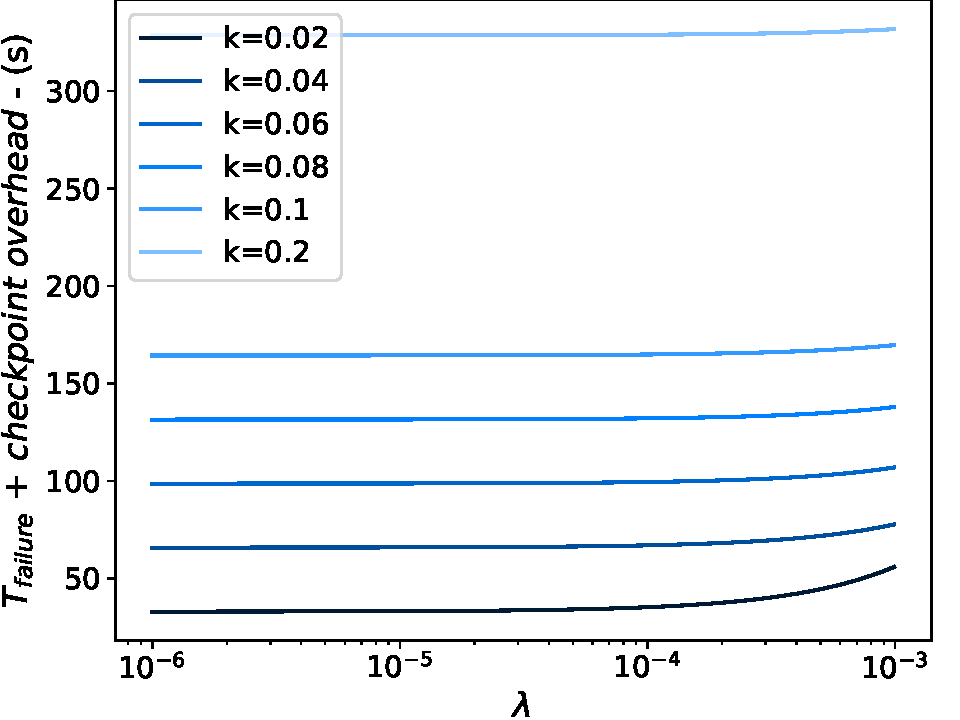
\includegraphics[width=0.49\textwidth]{avg_tot_ovhd_LU_C.pdf} }}\vspace{-1.1em}}
    {
    \subcaption[]{Benchmark: SP}
    \subfloat[\centering \textbf{(a)} Estimated mean overhead caused by the re-execution of application code in case of failure, varying $\lambda$ and $k$.]{{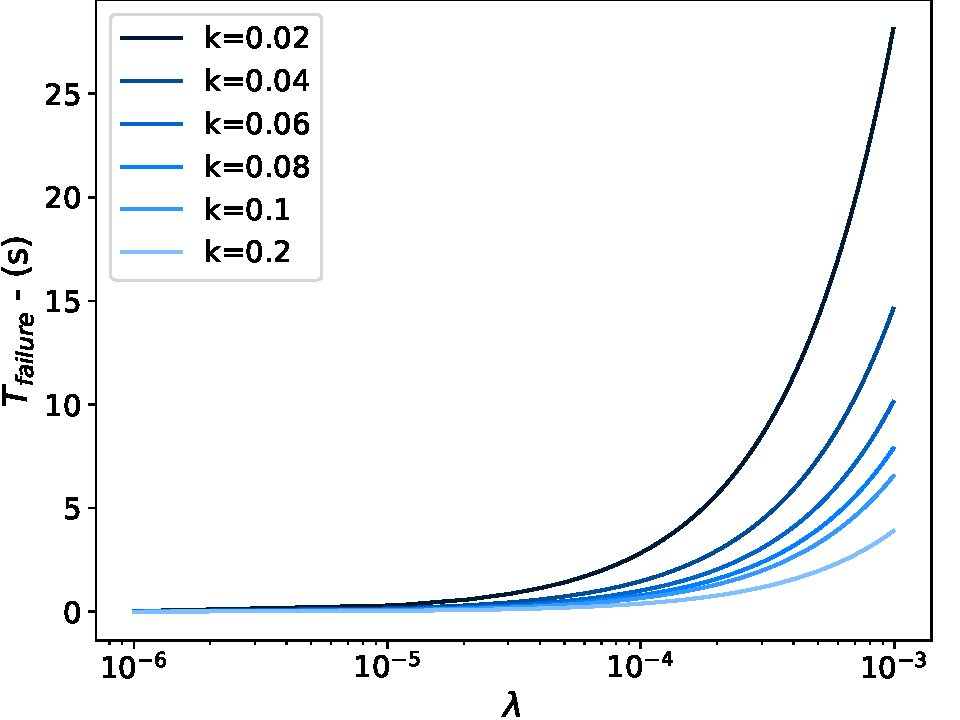
\includegraphics[width=0.49\textwidth]{avg_reset_time_SP_C.pdf} }}
    \subfloat[\centering \textbf{(b)} Sum of the value of \textbf{(a)} plus the checkpoint overhead, varying $\lambda$ and $k$.]{{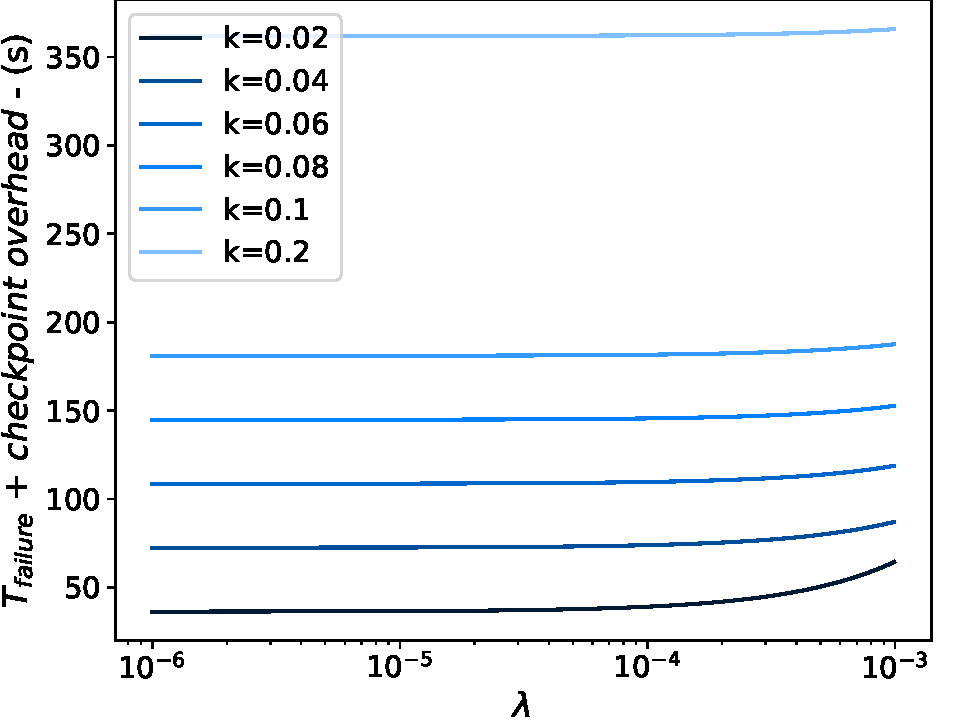
\includegraphics[width=0.49\textwidth]{avg_tot_ovhd_SP_C.pdf} }}}
    \caption{Plot of \textbf{(a)} $T_{failure}$, \textbf{(b)} $T_{failure}+checkpoint\ overhead$, varying $\lambda$ and $k$ - Problem size class C, estimate in seconds.}%
    \label{fig:comp_c}%
\end{figure}}

{\captionsetup[subfloat]{labelformat=empty}
\begin{figure}
    \centering
    {
    \subcaption[]{Benchmark: BT}
    \subfloat[\centering]{{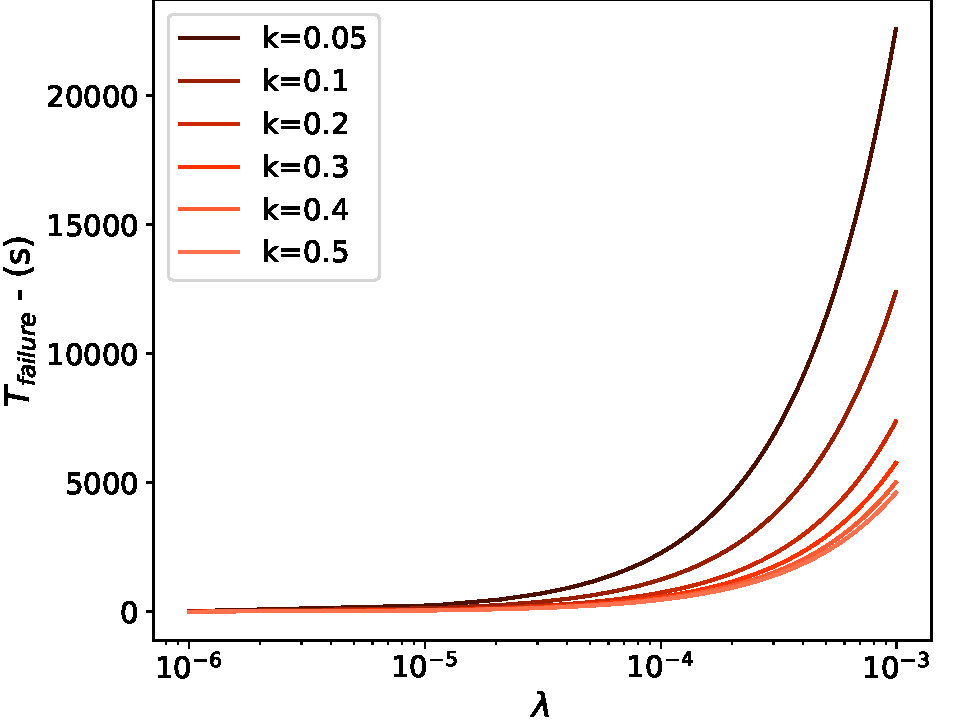
\includegraphics[width=0.49\textwidth]{avg_reset_time_BT_D.pdf} }}
    \subfloat[\centering]{{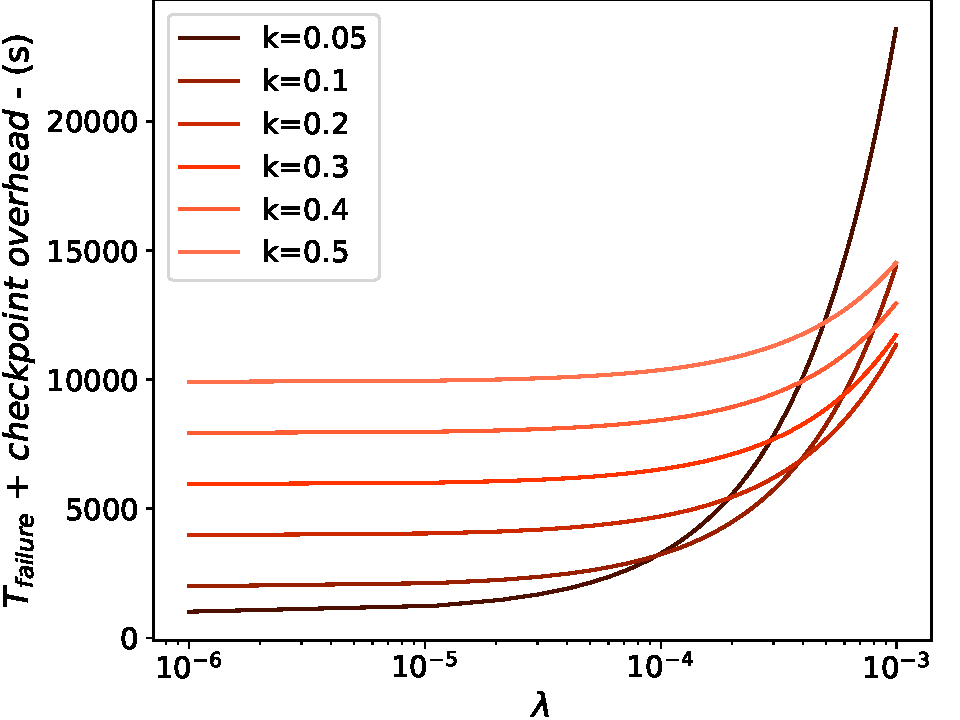
\includegraphics[width=0.49\textwidth]{avg_tot_ovhd_BT_D.pdf} }}\vspace{-1.1em}}
    {
    \subcaption[]{Benchmark: LU}
    \subfloat[\centering]{{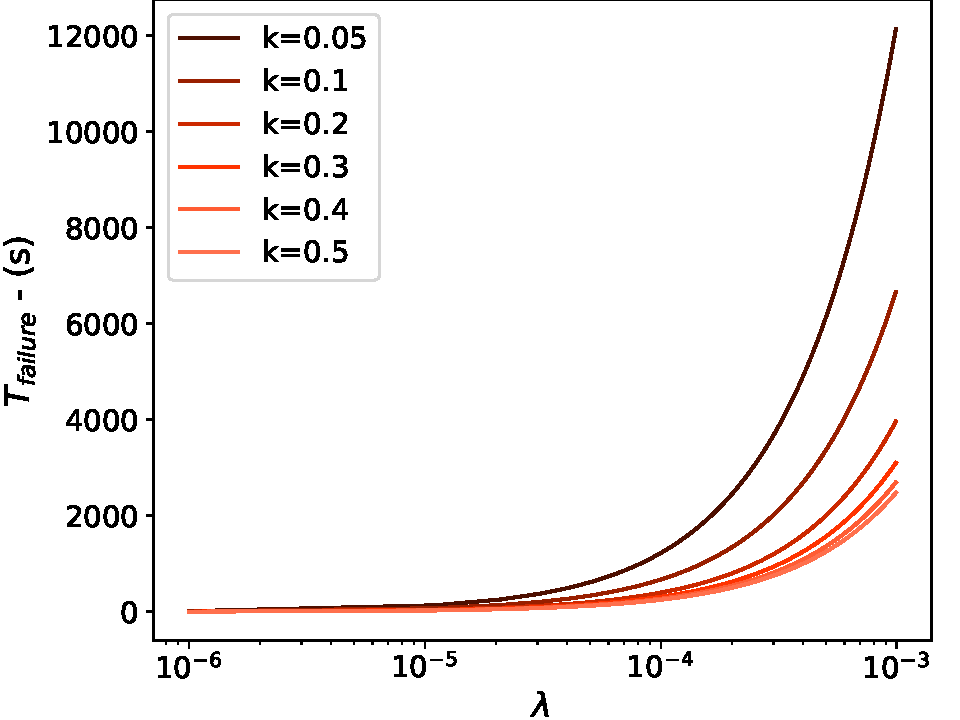
\includegraphics[width=0.49\textwidth]{avg_reset_time_LU_D.pdf} }}
    \subfloat[\centering]{{\includegraphics[width=0.49\textwidth]{avg_tot_ovhd_LU_D.pdf} }}\vspace{-1.1em}}
    {
    \subcaption[]{Benchmark: SP}
    \subfloat[\centering \textbf{(a)} Estimated mean overhead caused by the re-execution of application code in case of failure, varying $\lambda$ and $k$.]{{\includegraphics[width=0.49\textwidth]{avg_reset_time_SP_D.pdf} }}
    \subfloat[\centering \textbf{(b)} Sum of the value of \textbf{(a)} plus the checkpoint overhead, varying $\lambda$ and $k$.]{{\includegraphics[width=0.49\textwidth]{avg_tot_ovhd_SP_D.pdf} }}}
    \caption{Plot of \textbf{(a)} $T_{failure}$, \textbf{(b)} $T_{failure}+checkpoint\ overhead$, varying $\lambda$ and $k$ - Problem size class D, estimate in seconds.}%
    \label{fig:comp_d}%
\end{figure}}

{\captionsetup[subfloat]{labelformat=empty}
\begin{figure}
    \centering
    {
    \subcaption[]{Benchmark: BT}
    \subfloat[\centering]{{\includegraphics[width=0.49\textwidth]{perc_tot_ovhd_BT_C.pdf} }}
    \subfloat[\centering]{{\includegraphics[width=0.49\textwidth]{perc_tot_ovhd_BT_D.pdf} }}\vspace{-1.1em}}
    {
    \subcaption[]{Benchmark: LU}
    \subfloat[\centering]{{\includegraphics[width=0.49\textwidth]{perc_tot_ovhd_LU_C.pdf} }}
    \subfloat[\centering]{{\includegraphics[width=0.49\textwidth]{perc_tot_ovhd_LU_D.pdf} }}\vspace{-1.1em}}
    {
    \subcaption[]{Benchmark: SP}
    \subfloat[\centering \textbf{(a)} Problem size class C.]{{\includegraphics[width=0.49\textwidth]{perc_tot_ovhd_SP_C.pdf} }}
    \subfloat[\centering \textbf{(b)} Problem size class D.]{{\includegraphics[width=0.49\textwidth]{perc_tot_ovhd_SP_D.pdf} }}}
    \caption{Estimated percentage overhead caused by the sum of checkpointing time and time to recover from a failure, varying $\lambda$, on the execution of the sole application code.}%
    \label{fig:comp_perc}%
\end{figure}}
\newpage
\section{Reliam Resource Allocation Policy}
As explained in Section~\ref{sec:poldesign}, the Reliam Resource Allocation Policy is composed by two main components: the mathematical model behind the CPU quota allocation, based on a modification of the PID controller model, and the selection of the CPU cores, based on reliability criteria. The first component aims to reduce the CPU utilization, in order to favor applications parallelization, while the second one has been designed to improve the reliability of the hardware components, minimizing their aging. Thanks to the low interdependence of the two components, it has been possible to test their objectives separately. The results of the first set of experiments will show the behavior of the controller, depending on the tuning of the controlling parameters. In such regard, three different use cases will be provided as a guideline in the setting of the policy. In the second set of tests, the effectiveness of the reliability decisions of the policy will be evaluated and commented. For this purpose, DCworms has been used in order to simulate a multi-core system.

\subsection{CPU quota allocation}
In this section the guidelines for tuning the modified PID controller model will be provided and the evaluation of its effectiveness  will take place, considering three different use cases of the CPU quota allocation mechanism.

\subsubsection{PID controller parametric tuning properties}
PID controllers are one of the most widely and successfully used controllers in a variety of industrial areas \cite{1638134}.

As introduced in Section~\ref{sec:poldesign}, the PID controller is designed as a \emph{negative feedback model}, relying on proportional, integral and derivative contributions, weighted by coefficients, respectively, $k_p,\ k_i, \text{ and } k_d$. In their combination, they contribute to the control action $u$, as shown in the following expression:
\begin{align*}
u(t) = k_p\,\epsilon(t) + k_i\int\epsilon(t)\,dt + k_d\,\frac{d\,\epsilon(t)}{dt}    
\end{align*}
where $\epsilon(t)$ represents the error at time $t$.

In order to properly tune a PID controller, we need to focus on four of its properties \cite{zhong2006pid}:
\begin{description}
\item[Rise Time:] time taken for the output to rise beyond 90\% of the desired level for the first time.
\item[Overshoot:] how much the the peak level is higher than the steady state, normalized against the steady state.
\item[Settling Time:] time taken for the system to converge to its steady state.
\item[Steady-State Error:] difference between the steady-state output and the desired output.
\end{description}

The increasing of each of the controller coefficients, $k_p,\ k_i, \text{ and } k_d$ has a different effect on each of the above mentioned properties. A summary of such effect is provided by Table~\ref{tab:pideffect}.

\begin{table}[t]
    \centering
    \begin{tabular}{|c||c|c|c|c|}
        \cline{2-5}
         \multicolumn{1}{l||}{}& \emph{Rise Time} & \emph{Overshoot} & \emph{Settling Time} & \emph{S-S Error}\\
        \hline\hline
        $k_{p}$ & Decrease & Increase & - & Decrease\\
        $k_{i}$ & Decrease & Increase & Increase & Eliminate\\
        $k_{d}$ & - & Decrease & Decrease & - \\
        \hline
    \end{tabular}
    \caption{Effect of the increasing of the controller parameters on the PID properties \cite{zhong2006pid}.}
    \label{tab:pideffect}
\end{table}

\subsubsection{The modified PID controller}
As deeply examined in Section~\ref{sec:poldesign}, in this work we made some changes to the PID controller in order for it to better fit the resource allocation problem.

In the following, the reached CPU quota assignment model is summarized:

\begin{enumerate}[label=-]
    \item Control variable: $cv$
    \item Process variable: $\Delta$
    \item Setpoint: $\overline{\Delta}$
    \item Error: $\epsilon$
\end{enumerate}
where:
\begin{align*}
    \renewcommand{\arraystretch}{3}
    \begin{array}{ll}
        cv &= 
        \begin{cases}
                k_{p}*\epsilon_r + k_{i}*\sum_{k\in R}\epsilon_{k} + k_d*(\epsilon_{r}-\epsilon_{r-1}) & \qquad \mbox{if } \epsilon\neq 0 \\
        	    0 & \qquad\mbox{otherwise} 
        \end{cases}\\
        \Delta &= 
            \begin{cases}
        	    CPU_{A} - CPU_{U} \hfill& \qquad \mbox{if } CPU_{A} > CPU_{U} \\
        	    \Delta_{NEG} &\qquad \text{otherwise}
    	    \end{cases}\\
    	    \epsilon &=
    	    \begin{cases}
        	    \overline{\Delta} - \Delta &\qquad\mbox{if } |\overline{\Delta}-\Delta| \geq \overline{\Delta}\mbox{}\\
        	    0 &\qquad \mbox{otherwise}
    	    \end{cases}
	\end{array}
\end{align*}

In our model, the proportional, integral and derivative coefficients, respectively, $k_p,\ k_i, \text{ and } k_d$, need to be properly tuned taking into consideration the target application. The tuning of such parameters is highly dependent on the workload and the resource availability in the system, as much as on the priority assigned to each application and the degree of parallelization desired for the system.

Although the mathematical model presented by this work shows an essential difference with respect to the simple PID controller model, due to the resetting of the integral and derivative contributions in the case of $\epsilon=0$, the effects of the controlling coefficients summarized in Table~\ref{tab:pideffect} nonetheless apply. Nevertheless, some considerations need to be made. Since applications are usually limited in time and not always constant at steady state, in this application area the concept of Steady-State Error might not be significant and the contribution of $k_{i}$ might not lead to its elimination. Moreover, Rise Time highly depends on the initial CPU quota assignment $CPU_{A_{ini}}$ which might be a straight away overshooting, hence, it is significant only in the case of $CPU_{A_{ini}} < CPU_{U_{ideal}}$, where the second term is the desired output of the policy. Also Settling Time, in the presented implementation, acquires a slight different meaning. Since the controller contributions are reset every time $\epsilon=0$ and, in any case, a steady-state does not always exist due to the possible variable workload of the application, we will refer, with Settling Time, to the first time the output of the controller matches the set point.

As anticipated above, a \emph{unique} optimal tuning of the three parameters of the controller does not exist, since it depends on the objective tried to be reached. In the following, three reasonable scenarios will be considered:
\begin{description}
\item[Scenario 1: massively parallel system.] Consider a system with limited computational resources with respect to the amount of parallel application executing simultaneously: the occurrence of a significant overshooting for an application might result in a waste in performance for the others, constrained for no reason with a CPU quota lower than the required.
\item[Scenario 2: mixed application priority system.] Take into account a system characterized by a wide number of computational resources and a time constrained prioritized application running on it: in this case, overshooting would not represent a problem as big as an extended rising time. 
\item[Scenario 3: long lasting applications system.] Consider a long lasting application with recurring small variations in the workload: we might want that, when such fluctuations occur, the CPU quota adjusts accordingly, avoiding big overshooting and minimizing the settling time.
\end{description}

Given the considerations expressed above, an analysis regarding the variation of the controlling parameters results necessary in the use of the Reliam Resource Allocation Policy. For this reason, an experimental characterization of the three above mentioned scenarios will be provided and commented.

For the experimental evaluation of the CPU quota allocation of the Reliam Resource Allocation Policy, we chose the PARSEC benchmark \emph{Fluidanimate} launched with two threads, set $\Delta_{NEG}=25$, $\overline{\Delta}=5$ and the invocation period of the policy to 4 seconds. We performed our experiments knowing that the CPU usage of the application at issue is approximately $CPU_{U}= 200$.

\begin{figure}[t]
    \centering
    \includegraphics[width=0.8\textwidth]{delta_kp=0.5_ki=0_kd=0_def=100.pdf}
    \caption{\emph{Scenario 1}. Observed $\Delta$ at each invocation $r$ of the Reliam Resource Allocation Policy, setting $k_{p}=0.5\text{ and }k_{i}=k_{d}=0.0$. The blue area corresponds to the values of $\Delta$ such that $\epsilon=0$, the dashed line to $\overline{\Delta}$.}
    \label{fig:pid500}
\end{figure}

To match \textbf{Scenario 1}, we firstly consider an initial assigned CPU quota $CPU_{A_{ini}}=100$, since it is reasonable that an initial underestimation of the quota assignment is preferred in such conditions. To reach the objective, we set the controller up as purely proportional, i.e. eliminating the integral and derivative contributions. We expect from this settings a low\footnote{Lower than half of the absolute value of $\Delta_{NEG}$} or non-existent overshooting, due to the absence of the integral contribution.

We set the parameters as follows:
\begin{align*}
    k_p = 0.5 \quad k_i = 0.0 \quad k_d = 0.0
\end{align*}

The plot of the observed value of $\Delta$ at each invocation $r$ of the policy is shown in Figure~\ref{fig:pid500}. The underestimation of the CPU quota assignment is visible from the plot in the initial points, highlighted in red to be distinguished from the ones in green, producing $\epsilon=0$, hence, a correct assignment of the CPU quota. Those points correspond to the invocations of the policy in which the application uses all of the assigned resources, thus, an under-assignment is assumed and the value of $\Delta$ is approximated to $\Delta_{NEG}$ for a balanced functioning of the controller.

From the above mentioned Figure, it is possible to extract information about the PID properties discussed above.

As expected, no overshooting is present in the output of the controller, whose rising time, coinciding with the settling time, equals 8 invocations of the policy. In this scenario, no needless loss in terms of resource allocation is caused to other parallel applications, at the expenses of an initial under allocation for the one at issue. This approach favors the minimization of CPU utilization.

Starting from the previous settings, we consider a context more similar to \textbf{Scenario 2}. In this case, it is of greater importance to provide the application at issue with the needed CPU quota as soon as possible. Following the guidelines of Table~\ref{tab:pideffect}, we increase the value of $k_i$ leaving the other two coefficients unchanged.

The new setting becomes:
\begin{align*}
    k_p = 0.5 \quad k_i = 0.3 \quad k_d = 0.0
\end{align*}

The results of this configuration are shown in Figure~\ref{fig:pid530}.
As in the previous scenario, we identify the underestimation of the CPU quota in the initial points of the plot, characterized by $\Delta=\Delta_{NEG}$. Differently from before, at the fourth invocation, we observe a positive value of $\Delta$, exceeding the admissible range, represented by the blue area. Such points correspond to an over-assignment of CPU quota, hence, to real values of $\Delta$, which does not need to be approximated with $\Delta_{NEG}$ anymore. From Figure~\ref{fig:pid530}, we can observe a large overshooting, which distances $\Delta$ from the setpoint of 45 units. Although the settling time corresponds with the ninth invocations of the policy, the application have at its disposal all the needed resources already at invocation 4. This approach favors the prioritization of the resource assignment for the application at issue, which is provided with an overestimation of its expected usage. System-wide, this kind of approach might result in a possible deprivation of CPU quota for the applications parallel to the one at issue. In systems in which one main application needs to run with maximum priority with respect to the others, a configuration similar to the one just analyzed is to be considered for the former, while using an approach like the one described in Scenario~1 for the latters.
\begin{figure}[t]
    \centering
    \includegraphics[width=0.8\textwidth]{delta_kp=0.5_ki=0.3_kd=0_def=100.pdf}
    \caption{\emph{Scenario 2}. Observed $\Delta$ at each invocation $r$ of the Reliam Resource Allocation Policy, setting $k_{p}=0.5\text{, }k_{i}=0.3\text{ and }k_{d}=0.0$. The blue area corresponds to the values of $\Delta$ such that $\epsilon=0$, the dashed line to $\overline{\Delta}$.}
    \label{fig:pid530}
\end{figure}

\begin{figure}[t]
    \centering
    \includegraphics[width=0.8\textwidth]{delta_kp=0.3_ki=0_kd=0.3_def=200.pdf}
    \caption{\emph{Scenario 3}. Observed $\Delta$ at each invocation $r$ of the Reliam Resource Allocation Policy, setting $k_{p}=0.3\text{, }k_{i}=0.0\text{ and }k_{d}=0.3$. The blue area corresponds to the values of $\Delta$ such that $\epsilon=0$, the dashed line to $\overline{\Delta}$.}
    \label{fig:pid303}
\end{figure}

Finally, to simulate \textbf{Scenario 3}, we resorted to the characteristic differentiating our model from a simple PID controller: the resetting of the integral and derivative contributions each time the annulment of the error is reached. This property has the same effect of resetting the controller with a new $CPU_{A_{ini}}$, i.e. the value that has lastly guaranteed $\epsilon=0$. Since, in the case of a long lasting application, it is reasonable to consider as negligible the first settling time, we simulate the operating application providing to the controller $CPU_{A_{ini}}=200$, i.e. a value \emph{close enough} to the CPU quota our benchmark is able to use.

Following the guidelines provided by Table~\ref{tab:pideffect}, we lower $k_p$ and $k_i$ to lower Overshooting, and increased $k_d$ to decrease Settling Time.

The resulted settings lead to a PD controller with parameters:
\begin{align*}
    k_p = 0.5 \quad k_i = 0.0 \quad k_d = 0.3
\end{align*}

Figure~\ref{fig:pid303} shows the results of the last experiment. The low\footnote{With respect to the other scenarios.} under-estimation of the CPU quota allocation can be inferred from the speed at which $\Delta$ goes from negative to positive values. This transition happens in just one invocation: this verifies the closeness between $CPU_{A_{ini}}$ and the real CPU quota requirement of the application. As expected, the registered overshoot results low, just 11 units of $\Delta$, and settling time corresponds to just 3 invocations of the policy. 


\subsection{CPU cores selection}
This section will focus on the experiments performed on the \emph{Reliam Resource Allocation Policy} to test the effectiveness of the CPU cores selection.

As anticipated above, DCworms has been exploited to test the policy on a multi-node scale.

We set the environment in order to simulate a system composed of 4 nodes with 16 processors each, for a total of 64 CPUs. On this system we simulated the execution of 256 running tasks.

Moreover, we excluded from the simulation any kind of checkpointing backup, i.e. if a failure occurs in the processing element used by the application, it goes back to the start and performs again all the computation.

As explained in Section~\ref{sec:poldesign}, the \emph{Reliam Resource Allocation Policy} is able to make two kinds of reliability-aware decisions:
\begin{enumerate}[label={\arabic*)}]
    \item In the case of a non-full-loaded system, it delegates the execution of the running applications to the \emph{most reliable} cores, idling the left ones;
    \item In the case of an application bound solely to \emph{non-reliable} cores, it freezes the execution and migrates the application to \emph{more reliable} cores, if any.
\end{enumerate}

We neglected the simulation of the decision described in 1), due to the triviality of the evaluation of the effectiveness. If an application runs only on the most reliable cores, for construction, it minimizes the occurrence of failures, without providing any worsening to the reliability of the \emph{critical} cores.
Conversely, we evaluated the effectiveness of the decisions described in 2).

We simulated a workload almost saturating the computational resources, with a total execution time, in absence of failures, $T_{exc\_tot}$, equal to 200 invocations of the policy. We performed our experiments considering different failure rates. More specifically, we selected five different Mean Time Between Failure (MTBF), corresponding to a number of invocations such to verify the following equalities:
\begin{itemize}
    \item $\frac{T_{exc\_tot}}{MTBF}=4$
    \item $\frac{T_{exc\_tot}}{MTBF}=5$
    \item $\frac{T_{exc\_tot}}{MTBF}=6$
    \item $\frac{T_{exc\_tot}}{MTBF}=7$
    \item $\frac{T_{exc\_tot}}{MTBF}=8$
\end{itemize}

Moreover, we defined two criticality thresholds, as described in Section~\ref{sec:dcworms}. Firstly we set such threshold to 70\%. This setting implies for the policy to mark a processing unit as \emph{critical} when such \emph{criticality threshold} is reached.

\begin{figure}[t]
    \centering
    \subfloat[\centering Criticality threshold equal to 70\%. ]{{\includegraphics[width=0.55\textwidth]{exc_time_rel=70.pdf} }}
    \\\hspace{1em}
    \subfloat[\centering Criticality threshold equal to 80\%.]{{\includegraphics[width=0.55\textwidth]{exc_time_rel=80.pdf} }}
    \caption{Execution time (expressed in number of invocations) provided by basic policy (blue bars) and the Reliam Resource Allocation Policy (orange bars).}
    \label{fig:exc}%
\end{figure}

We collected data regarding execution time and peak temperature of the processors. Then we performed the same experiments moving the criticality threshold to 80\%. Figures~\multiref{fig:exc}{fig:af} show the data collected from the simulation of the workload using the \emph{Reliam Resource Allocation Policy}, comparing them to the ones extracted from the execution of the same workload using a simple policy, performing migration only in case of failure.

Figure~\ref{fig:exc} shows the execution time, expressed in number of invocations of the policy, obtained with and without the reliability decisions of the \emph{Reliam Resource Allocation Policy}. In both cases, characterized, respectively, by a criticality threshold equal to 70\% and to 80\%, we observed in a mitigation in the loss of performance proportional to the injected failure rate. Thanks to the reliability-aware decisions, the application have a bigger probability of not getting bound to cores considered more prone to failures, hence, the re-execution of the application code happens with a lower frequency, conferring, in the tested cases, a mitigation of the performance loss ranging between 8\% and and 22\% in the case of criticality threshold equal to 70\%, while between 7\% and 14\%, in the case of criticality threshold equal to 80\%.

\begin{figure}[t]
    \centering
    \includegraphics[width=0.8\textwidth]{degradation.pdf}
    \caption{Performance degradation between criticality thresholds 80\% and 70\% .}
    \label{fig:degradation}
\end{figure}

Another interesting insight provided by the tests is represented by the comparison of the two policies in the different reliability scenarios. In the case of criticality threshold equal to 70\%, the Reliam Resource Allocation Policy presents a lower degradation in terms of performance with respect to the 80\% case. In the best tested case, represented by $\frac{T_{exc\_tot}}{MTBF}=4$, the worsening in performance observed by comparing the execution time provided by each policy with the different criticality threshold is about the same (19\% without Reliam, 18\% using Reliam). For $\frac{T_{exc\_tot}}{MTBF}=8$, the results of the policy without reliability control in the case of criticality threshold equal to 70\% presented a worsening of the performance equal to the 40\% of the performances registered with criticality threshold equal to 80\%. Considering the same scenarios, introducing the reliability-aware decisions, we observe a worsening of only 34\%. Such results are summarized in Figure~\ref{fig:degradation}.


\begin{figure}[t]
    \centering
    \subfloat[\centering Criticality threshold equal to 70\%.]{{\includegraphics[width=0.5\textwidth]{peak_temp_rel=70.pdf} }}
    %\\\vspace{1em}
    \subfloat[\centering Criticality threshold equal to 80\%.]{{\includegraphics[width=0.5\textwidth]{peak_temp_rel=80.pdf} }}
    \caption{Observed peak temperature (expressed in $^\circ$C) provided by the basic policy (blue bars) and the Reliam Resource Allocation Policy (orange bars).}
    \vspace{-0.4em}
    \label{fig:peak}%
\end{figure}

As mentioned above, we also collected data regarding the peak temperature reached by the CPUs during the execution of the workload, with and without the reliability decisions of the Reliam Resource Allocation Policy. Figure~\ref{fig:peak} summarizes such observation with the two tested criticality threshold. From the plots, we can notice that, in both settings, the execution without reliability control presents an ascending trend proportional to the injected failure rate. On the contrary, the reliability control invert this trend.

Moreover, it can be observed that, for $\frac{T_{exc\_tot}}{MTBF}=4$, corresponding to the lowest tested failure rate, for criticality threshold equal to 80\%, using the basic policy, we register a peak of 90$^\circ$C, higher than the one reached at 70\%. Also this trend is not followed using the Reliam Resource Allocation Policy, which provides the same and lower thermal values in both the reliability scenarios. 

We used such results to evaluate the contribution of the collected thermal stress in the wear out of the hardware components. To do so, we computed the \emph{acceleration factor}, a metric derived from the Arrhenius equation. The Arrhenius equation describes the dependence on the temperature of the \emph{rate constant}, $k$, of a chemical reaction. It is defined as:
\begin{align*}
    k = Ae^{-\frac{E_A}{RT}}
\end{align*}
where $A$ is a constant dependent on the reaction, $E_A$ is the activation energy, $R$ is the universal gas constant, and $T$ is the temperature expressed in Kelvin.
The acceleration factor consists in the ratio of a degradation rate at an elevated temperature and a lower field usage one, hence in the ratio of the Arrhenius equation evaluated in the two above mentioned values of temperature. Such metric is implemented in the \verb|libhwrel|, the hardware reliability monitor integrated in BarbequeRTRM, upon which an overview has been provided in the {\hyperref[sec:coresel]{design section of the cores selection}}. Algorithm~\ref{alg:acc_fac} shows the implementation of the function \verb|GetAccelerationFactor()|, as implemented in the \verb|libhwrel|: the used parameters refer to Intel CPUs with Skylake architecture. 

\begin{algorithm}
    \SetKwInput{KwInput}{Input}
    \SetKwInput{KwOutput}{Output}              % set the Output
    %\DontPrintSemicolon
    \BlankLine

    \KwInput{Current temperature \emph{temp}}

    \KwOutput{Acceleration factor \emph{af}}
    %\BlankLine
    \algrule
    

\BlankLine
\SetKwFunction{Funcs}{GetAccelerationFactor}
\SetKwProg{Fn}{double}{:}{}
\Fn{\Funcs{\KwSty{float} temp}}{
    \KwSty{double} act\_energy = 0.7\;
    \KwSty{double} boltzmann = 8.617333262145 * (1 / pow(10, 5))\;
    \KwSty{double} t\_use = 328.0\;
    \KwSty{double} t\_stress = temp + 273.15\;
    \KwSty{double} af\;
    \KwSty{double} exp = (act\_energy / boltzmann) * (1.0 / t\_use - 1.0 / t\_stress)\;
    \KwSty{double} af = pow(e, exp)\;
    \KwRet af\;
 }
    \BlankLine
   \caption{Computation of the acceleration factor.}
   \label{alg:acc_fac}
\end{algorithm}


Considering the peak temperatures reached in the simulated system, we computed the acceleration factor produced by the two policies on the most critical processing units in both reliability scenarios.
\begin{figure}[t]
    \centering
    \subfloat[\centering Criticality threshold equal to 70\%.]{{\includegraphics[width=0.55\textwidth]{af_70.pdf} }}
    \vspace{1.1em}
    \subfloat[\centering Criticality threshold equal to 80\%.]{{\includegraphics[width=0.55\textwidth]{af_80.pdf} }}
    \caption{Acceleration factor produced by the basic policy (blue bars) and the Reliam Resource Allocation Policy (orange bars).}
    \label{fig:af}%
\end{figure}

 Figure~\ref{fig:af} summarizes the results of such calculation. We can observe the substantial difference between the two curves characterized, respectively, by the absence, in blue, and the presence, in orange, of the reliability control. In the case of criticality threshold equal to 70\%, in the best case, the computed acceleration factor produced without the reliability decisions more than doubles the one observed using it. In the case of criticality threshold equal to 80\%, it more than triples it.  In both plots, in the worst case scenario, represented by $\frac{T_{exc\_tot}}{MTBF}=8$, the acceleration factor produced by the basic policy is higher than the quintuple of the one registered with the Reliam Resource Allocation Policy. 

These results prove the effectiveness of the reliability-aware decisions made by the Reliam Resource Allocation Policy. They not only improve the reliability of the application execution, providing \emph{safer} application-CPU bindings, which lower the probability of using an already worn out processor, but also, slow down the wear out of the hardware components, reducing the acceleration of the reliability degradation in terms of Mean Time To Failure (MTTF) caused by thermal stress.

\cleardoublepage
%
\phantomsection
%
%\addcontentsline{toc}{chapter}{Conclusions}
%
\chapter{Conclusions}
%
\markboth{Conclusions}{Conclusions}	% headings
%
\label{cap:conclusions}

In this chapter a summary of the work presented by this thesis and of the results of the tests performed on it will be provided. Finally, an overview on the possible future works, able to extend the \emph{Dynamic Checkpoint Rate Tuning} and the \emph{Reliam Resource Allocation Policy}, will be furnished.

\section{Conclusions}
This thesis presents our contribution to the mitigation of the reliability problem in HPC systems, which represents a matter of major concern with the advance in technology and popularity of such systems in a wide area of applications.

We firstly described the \emph{Dynamic Checkpoint Rate Tuning}, an application-aware checkpoint scheduler, whose objective relies in the maximization of the fault tolerance with utmost attention to its impact on the performance.

We provided the possibility for the user to set an upper bound $k$, defined as the tolerated overhead with respect to the non-faulty execution of the sole application code. The value of $k$ is considered during the checkpoint scheduling, based on the prediction of the checkpoint time, in order not to lower the desired application performance.
 
In the case of smaller sized problem applications, such approach resulted effective in all the tested levels of system criticality. For such kind of workload, setting a low value of $k$ (up to the 2\% of overhead) resulted \emph{safe} with respect to the performance counting, which continued to be only slightly undermined, even in highly critical systems (i.e. with failure rate equal to $10^{-3}$ failures per hour). In such case, \emph{restart time} showed a worsening of the performance of less than 2\% in the worse tested case\footnote{$k=0.02$, i.e. maximum tolerated overhead of 2\%.}, a weight halved already with $k=0.04$. Slightly different results have been achieved for bigger sized problems. In this scenario, tested with a minimum tolerated checkpoint overhead of $k=0.05$, we registered a negligible worsening of the performance given by restart time in averagely and highly reliable systems (i.e. systems with failure rate lower than $10^{-4}$ failures per hour), while an inversion of the trend has been observed for higher failure rates. In this case, lower values of $k$ led to a cumulative performance worsening higher than the one obtained with higher values of $k$. Considering $k=0.05$, for all three evaluated benchmarks, we observed a worse performance counting, due to \emph{restart time}, around values of failure rate equal to $10^{-4}$, where higher values of $k$ provided better performance. 
Conclusions deduced from such experiments are that, if, for smaller problem sizes, lower values of $k$ lead to lower worsening of the performance in all the realistic range of system criticality levels, for bigger problem sizes, an extra care is to be grant in the case of reliability critical system to not incur in high performance worsening caused by the time to recover from failures.

The second pillar this thesis has been built on is the design and implementation of the \emph{Reliam Resource Allocation Policy}. Such policy, periodically invoked, assigns a controller to each running application in order to iteratively adapt the allocation of the CPU quota to its computational need. Moreover, it makes binding decisions in order to improve application and system reliability. 

We firstly provided the experimental evaluation of the computation of the CPU quota allocation mechanism. Three practical scenarios have been described, analyzing the produced rise time, overshoot and settling time provided by the different tuning of the controlling parameters. It has been observed that, increasing the sole proportional contribution, a slow annulment of the error is achieved, favoring the minimization of the overshooting. This approach is to be preferred in the case of \emph{massively parallel systems}, in which the minimization of the CPU utilization is key for the overall performance. Conversely, the increase of the integral contribution significantly reduces the rise time, while enlarging the overshoot. A use case of such tuning might be represented by the willingness of prioritizing the execution performance of an application over the others. Lastly, increasing the derivative contribution in place of the integral one, resulted in the reduction of overshooting and a consequently small settling time, a desired behavior in the case of batch application, whose workload tend to slightly vary over time.

Finally, we evaluated the effectiveness of the reliability-aware decisions, by applying them to a simulated multi-node system. We observed that the use of the Reliam Resource Allocation Policy, promoting the binding with the most reliable processing units, favors the reduction in the number of occurred failure, hence, in the application total time. Moreover, it significantly lowers the \emph{acceleration factor} of the resources presenting the highest temperature, slowing down the degradation in terms of MTTF due to thermal stress.

\section{Future work}
The work, as proposed by this thesis, focuses on CPU based systems. A natural extension which needs to be integrated is the support for heterogeneous systems. As anticipated in {\hyperref[cap:stateofart]{Chapter 2}}, at the time of writing, a stable software tool able to perform checkpoints of GPU applications does not exist: when such technology will become available, the \emph{Dynamic Checkpoint Rate Tuning} might be integrated with a support in such regard. As for FPGA, a partnership with \emph{CeRICT (Centro Regionale Information Communication Technology)} is already in progress, to integrate the already existing \verb|libacre|, the library currently overseeing the checkpointing in the BarbequeRTRM, with a support on such technology. When this work will be finalized, FPGA checkpointing might be included in the \emph{Dynamic Checkpoint Rate Tuning}.

Moreover, the current implementation of the \emph{Dynamic Checkpoint Rate Tuning} presents a limitation represented by the degradation of the performance of big problem sized workload in case of unreliable systems. Since failure rate is reasonable to change over time, the initial choice of $k$ might not be suitable for the entire execution time of the application. In this regard, a possible future work is represented by the integration in the framework of a run time and/or input profiling of the application workload, able, given the reliability information provided by the \verb|libhwrel|, to predict at which failure rate the value of $k$ stops being proportional to the gain in performance. In this way, it will be possible for the \emph{Dynamic Checkpoint Rate Tuning} to modify accordingly the value of $k$, in order not to lose the performance goal.

Another natural continuation of our project is represented by the support of custom accelerators in the \emph{Reliam Resource Allocation Policy}. At the time of writing, it is not possible to adapt the concept of \emph{quota} to these technologies, nevertheless, it is still possible to apply the proposed reliability-aware decisions of the policy at processing unit level, in order to contrast the wear out of such hardware components.
%
%
% ------------------------------------------------------------------------ %
% 	BACKMATTER
% ------------------------------------------------------------------------ %
%
\cleardoublepage
%
\backmatter
%
%
\cleardoublepage
%\nocite{*}	% anche riferimenti non citati
\printbibliography

%
%% ------------------------------------------------------------------------ %
% !TEX encoding = UTF-8 Unicode
% !TEX TS-program = pdflatex
% !TEX root = ../Tesi.tex
% !TEX spellcheck = it-IT
% ------------------------------------------------------------------------ %
%
% ------------------------------------------------------------------------ %
% 	DICHIARAZIONE
% ------------------------------------------------------------------------ %
%
\cleardoublepage
%
\phantomsection
%
\pdfbookmark{Dichiarazione}{Dichiarazione}
%
\chapter*{Dichiarazione}
%
\thispagestyle{empty}
%
\lipsum[1]

\bigskip
 
\noindent\textit{\myLocation, \myTime}

\smallskip

\begin{flushright}
    \begin{tabular}{m{6cm}}
        \\ \hline \\
        \centering\myName \\
    \end{tabular}
\end{flushright}
%
% ------------------------------------------------------------------------ %
%
% ------------------------------------------------------------------------ %
% 	END DOCUMENT
% ------------------------------------------------------------------------ %
%
\end{document}
%
% ------------------------------------------------------------------------ %